% Options for packages loaded elsewhere
\PassOptionsToPackage{unicode}{hyperref}
\PassOptionsToPackage{hyphens}{url}
%
\documentclass[
]{book}
\usepackage{amsmath,amssymb}
\usepackage{lmodern}
\usepackage{iftex}
\ifPDFTeX
  \usepackage[T1]{fontenc}
  \usepackage[utf8]{inputenc}
  \usepackage{textcomp} % provide euro and other symbols
\else % if luatex or xetex
  \usepackage{unicode-math}
  \defaultfontfeatures{Scale=MatchLowercase}
  \defaultfontfeatures[\rmfamily]{Ligatures=TeX,Scale=1}
\fi
% Use upquote if available, for straight quotes in verbatim environments
\IfFileExists{upquote.sty}{\usepackage{upquote}}{}
\IfFileExists{microtype.sty}{% use microtype if available
  \usepackage[]{microtype}
  \UseMicrotypeSet[protrusion]{basicmath} % disable protrusion for tt fonts
}{}
\makeatletter
\@ifundefined{KOMAClassName}{% if non-KOMA class
  \IfFileExists{parskip.sty}{%
    \usepackage{parskip}
  }{% else
    \setlength{\parindent}{0pt}
    \setlength{\parskip}{6pt plus 2pt minus 1pt}}
}{% if KOMA class
  \KOMAoptions{parskip=half}}
\makeatother
\usepackage{xcolor}
\usepackage{longtable,booktabs,array}
\usepackage{calc} % for calculating minipage widths
% Correct order of tables after \paragraph or \subparagraph
\usepackage{etoolbox}
\makeatletter
\patchcmd\longtable{\par}{\if@noskipsec\mbox{}\fi\par}{}{}
\makeatother
% Allow footnotes in longtable head/foot
\IfFileExists{footnotehyper.sty}{\usepackage{footnotehyper}}{\usepackage{footnote}}
\makesavenoteenv{longtable}
\usepackage{graphicx}
\makeatletter
\def\maxwidth{\ifdim\Gin@nat@width>\linewidth\linewidth\else\Gin@nat@width\fi}
\def\maxheight{\ifdim\Gin@nat@height>\textheight\textheight\else\Gin@nat@height\fi}
\makeatother
% Scale images if necessary, so that they will not overflow the page
% margins by default, and it is still possible to overwrite the defaults
% using explicit options in \includegraphics[width, height, ...]{}
\setkeys{Gin}{width=\maxwidth,height=\maxheight,keepaspectratio}
% Set default figure placement to htbp
\makeatletter
\def\fps@figure{htbp}
\makeatother
\setlength{\emergencystretch}{3em} % prevent overfull lines
\providecommand{\tightlist}{%
  \setlength{\itemsep}{0pt}\setlength{\parskip}{0pt}}
\setcounter{secnumdepth}{5}
\usepackage{booktabs}
\usepackage{amsmath}
\usepackage[utf8x]{inputenc}
\usepackage{natbib}
\ifLuaTeX
  \usepackage{selnolig}  % disable illegal ligatures
\fi
\IfFileExists{bookmark.sty}{\usepackage{bookmark}}{\usepackage{hyperref}}
\IfFileExists{xurl.sty}{\usepackage{xurl}}{} % add URL line breaks if available
\urlstyle{same} % disable monospaced font for URLs
\hypersetup{
  pdftitle={Clusterización Funcional Espacial},
  pdfauthor={Nosotros},
  hidelinks,
  pdfcreator={LaTeX via pandoc}}

\title{Clusterización Funcional Espacial}
\author{Nosotros}
\date{2022-09-26}

\begin{document}
\maketitle

{
\setcounter{tocdepth}{1}
\tableofcontents
}
\hypertarget{prefacio}{%
\chapter*{Prefacio}\label{prefacio}}
\addcontentsline{toc}{chapter}{Prefacio}

La dependencia espacial en datos medio ambientales es un criterio influyente en procesos de agrupación, dado que los resultados obtenidos brindan información relevante. Como los métodos clásicos no consideran la dependencia espacial, al considerar esta estructura se producen resultados inesperados, proporcionando agrupaciones de curvas que pueden no ser similares en forma y/o comportamiento. En este trabajo se realiza la agrupación mediante el método k-medias modificado para datos funcionales correlacionados espacialmente aplicado a datos del Índice de Vegetación de Diferencia Normalizada (NDVI) de los páramos del Ecuador. Para esto se implementan índices de calidad que permitan obtener el número adecuado de grupos. Con base en la metodología desarrollada en el método de clasificación jerárquico para datos funcionales con correlación espacial, y dado que los datos funcionales pertenecen al espacio de Hilbert de funciones cuadrado-integrables; se desarrolla el análisis considerando la distancia entre curvas a través de la norma \(\mathcal{L}^2\), obteniendo una representación reducida de los datos a través de una base finita de tipo Fourier. Luego, se calcula el variograma empírico y se ajusta a un modelo teórico para así ponderar la matriz de distancia entre las curvas por el trazo-variograma y variograma multivariado calculado con los coeficientes de las funciones base, y esta matriz se utiliza para la agrupación de datos funcionales correlacionados espacialmente. Para la validación del método se realizaron varios escenarios de simulación, obteniéndose buenos resultados de correcta clasificación y se complementa con un caso de aplicación a datos del NDVI, donde se obtuvieron cinco regiones distribuidas latitudinalmente.

\hypertarget{introducciuxf3n}{%
\chapter{Introducción}\label{introducciuxf3n}}

Los métodos de agrupación tienen por objetivo identificar grupos homogéneos de observaciones que representan la realización de alguna variable aleatoria X (\protect\hyperlink{ref-Jaque}{\textbf{Jaque?}}), y en los cuales los miembros dentro de los grupos tienden a ser similares y distintos de otros miembros de otros grupos (\protect\hyperlink{ref-Romano}{\textbf{Romano?}}). Estos métodos también son conocidos como métodos de clasificación no supervisada, pues las observaciones no tienen asociadas ninguna etiqueta de grupo o categoría de forma previa (\protect\hyperlink{ref-Jain}{\textbf{Jain?}}); por lo cual, este tipo de métodos se utilizan con frecuencia para detectar patrones especiales en una base de datos, los cuales pueden tener interpretaciones convenientes por parte del usuario (\protect\hyperlink{ref-Jaque}{\textbf{Jaque?}}).

Uno de los métodos más populares de agrupación es el algoritmo k-medias, pues desde 1955 se ha venido utilizando y adaptando a miles de problemas en diferentes campos de las ciencias (\protect\hyperlink{ref-Jain}{\textbf{Jain?}}). Muchas de estas adaptaciones asumen que las observaciones de tipo escalar, espacial y multivariante, pueden ser representadas como puntos en un espacio Euclídeo de dimensión finita, pero cuando la dimensión del objeto es sumamente grande las realizaciones de la variable aleatoria X pueden tomar valores en un espacio infinito dimensional (\protect\hyperlink{ref-Jaque}{\textbf{Jaque?}}); este último tipo de dato es muy común, ya que hoy en día se pueden realizar mediciones en cada instante de tiempo y es conocido como dato funcional. Es así que, este problema se puede abordar desde el análisis de datos funcionales, pues su objetivo es inferir la estructura de los datos trabajando con su naturaleza de dimensión infinita sobre espacios de Hilbert (\protect\hyperlink{ref-Luz}{\textbf{Luz?}}).

Dado que el campo de aplicación es amplio para el uso de estos métodos, nos centraremos en el área medioambiental, pues en esta área se trabaja con datos temporales, los cuales según (\protect\hyperlink{ref-Elvira}{\textbf{Elvira?}}), también son considerados como datos funcionales. Aplicar un método de agrupación, omitiendo su estructura espacial, dará como resultado grupos en los cuales las curvas pueden no ser similares en forma y/o comportamiento (\protect\hyperlink{ref-Elvira}{\textbf{Elvira?}}). Para abordar este problema, hasta el momento se han propuesto métodos de agrupación como el jerárquico (\protect\hyperlink{ref-Hclust}{\textbf{Hclust?}}) y el dinámico (\protect\hyperlink{ref-Elvira}{\textbf{Elvira?}}), los cuales usan el trazo-variograma como medida de dependencia espacial, con la diferencia de que en el método jerárquico se realiza el cálculo de manera global, mientras que en el método dinámico se lo realiza de manera local; así, el método jerárquico usa la distancia euclidiana entre las curvas, mientras que el método dinámico usa la distancia euclidiana al cuadrado entre las curvas dentro de cada grupo (\protect\hyperlink{ref-Romano}{\textbf{Romano?}}). Al notar la escasez de opciones de métodos, así como la no implementación del método k-medias, contar con más opciones de agrupación que trabajen con este tipo de datos serán de gran ayuda; es por ello que en este trabajo se implementará el método k-medias para datos funcionales con correlación espacial, para lo cual se usará la metodología aplicada en (\protect\hyperlink{ref-Hclust}{\textbf{Hclust?}}), y para evaluar el desempeño del método propuesto, se realizarán varios escenarios de simulación, y posteriormente aplicar este método a los datos del NDVI de los páramos del Ecuador.

\hypertarget{motivaciuxf3n-de-datos-funcionales-espaciales}{%
\section{Motivación de datos funcionales espaciales}\label{motivaciuxf3n-de-datos-funcionales-espaciales}}

Cosas\ldots{}

\hypertarget{por-quuxe9-es-importante-el-anuxe1lisis-de-datos}{%
\section{Por qué es importante el análisis de datos}\label{por-quuxe9-es-importante-el-anuxe1lisis-de-datos}}

cosas\ldots{}

\hypertarget{data-1h}{%
\subsection{Data 1(H)}\label{data-1h}}

\hypertarget{data-2c}{%
\subsection{Data 2(C)}\label{data-2c}}

\hypertarget{data-3n}{%
\subsection{Data 3(N)}\label{data-3n}}

\hypertarget{estaduxedstica-espacial}{%
\chapter{Estadística espacial}\label{estaduxedstica-espacial}}

\hypertarget{preliminares}{%
\section{Preliminares}\label{preliminares}}

\hypertarget{funciuxf3n-aleatoria}{%
\subsection{Función Aleatoria}\label{funciuxf3n-aleatoria}}

Dado un dominio \(D\subset \mathbb{R}^n\) y un espacio de probabilidad \((\Omega,\mathcal{A},P)\), una función aleatoria es una función de dos variables \(Z(x,\omega)\) tal que para cada \(x\in D\), \(Z(x,.)\) es una variable aleatoria en \((\Omega,\mathcal{A},P)\). Por otro lado, \(Z(.,\omega)\), definido en \(D\) como la sección de la función aleatoria en \(\omega \in \Omega\) es una realización de la función aleatoria. La función aleatoria \(Z(x,\omega)\) se denota como \(Z(x)\) y una realización es representada por \(z(x)\) (\protect\hyperlink{ref-GeoJean}{\textbf{GeoJean?}}).

\hypertarget{proceso-estocuxe1stico}{%
\subsection{Proceso Estocástico}\label{proceso-estocuxe1stico}}

Según (\protect\hyperlink{ref-GeoJean}{\textbf{GeoJean?}}), una función aleatoria es llamada proceso estocástico cuando \(x\) varia en un espacio unidimensional como el tiempo; por otro lado, si \(x\) varia en más de una dimensión es conocido como campo aleatorio.

\hypertarget{proceso-espacial}{%
\subsection{Proceso Espacial}\label{proceso-espacial}}

Sea \(Z\) la variable aleatoria de interés y \(s\) su ubicación espacia. El proceso espacial es el proceso estocástico

\begin{align}
\{Z(s):s \in D\}
\end{align}

donde \(D \subset \mathbb{R}^d\) es el conjunto formado por todas las ubicaciones espaciales (\protect\hyperlink{ref-marta}{\textbf{marta?}}).

\hypertarget{proceso-temporal}{%
\subsection{Proceso Temporal}\label{proceso-temporal}}

Sea \(Z\) la variable aleatoria de interés y \(t\) el tiempo. El proceso temporal es el proceso estocástico

\begin{align}
\{Z(t):t \in D\}
\end{align}

donde \(D \subset \mathbb{R}\) es el conjunto formado por todos los instantes de tiempo (\protect\hyperlink{ref-marta}{\textbf{marta?}}).

\hypertarget{proceso-espacio-temporal}{%
\subsection{Proceso Espacio Temporal}\label{proceso-espacio-temporal}}

Sea \(Z\) la variable aleatoria de interés, \(s\) su ubicación espacial y \(t\) el tiempo de ocurrencia. Un proceso espacio-temporal es un proceso estocástico

\begin{align}
\{Z(s,t):(s,t) \in D \times D' \}
\end{align}

donde el conjunto \(D \subset \mathbb{R}^d\) es el conjunto de todas las ubicaciones espaciales y el conjunto \(D' \subset \mathbb{R}\) es el conjunto de todos los instantes de tiempo. Los conjuntos \(D\) y \(D'\) pueden ser continuos o discretos, fijos o aleatorios (\protect\hyperlink{ref-marta}{\textbf{marta?}}).

\hypertarget{clases-de-datos-espaciales}{%
\section{Clases de Datos Espaciales}\label{clases-de-datos-espaciales}}

Dependiendo de las características del dominio espacial \(D\) del proceso estocástico de interés, se tienen los siguientes tipos de datos espaciales principales, los cuales son geoestadística, datos de área o \textit{lattice}, procesos o patrones espaciales puntuales y datos georreferenciados.

\hypertarget{geoestaduxedstica}{%
\subsection{Geoestadística}\label{geoestaduxedstica}}

Es el conjunto de métodos aplicados a datos espaciales, donde las ubicaciones espaciales \(s\) provienen de un conjunto continuo y fijo \(D \subset \mathbb{R}^d\); cabe resaltar que el propósito de la geoestadística es la interpolación. Además, si el conjunto \(D\) no es continuo se puede llegar a obtener predicciones carentes de sentido, y se considera \(D\) fijo pues los puntos en el espacio se seleccionan a conveniencia o bajo un esquema de muestreo probabilístico (\protect\hyperlink{ref-Ramon}{\textbf{Ramon?}}).

\hypertarget{datos-de-uxe1rea}{%
\subsection{Datos de Área}\label{datos-de-uxe1rea}}

En este tipo de datos las ubicaciones espaciales pertenecen a un conjunto discreto contable y fijo \(D \subset \mathbb{R}^d\). Las ubicaciones pueden estar espaciadas regular o irregularmente, usualmente son irregulares pues sus separaciones no siguen un patrón predecible.(\protect\hyperlink{ref-Cressi}{\textbf{Cressi?}}).

\hypertarget{patrones-puntuales}{%
\subsection{Patrones Puntuales}\label{patrones-puntuales}}

En este caso, las ubicaciones espaciales pertenecen a un conjunto discreto o continuo y aleatorio \(D\subset \mathbb{R}^d\). Con este tipo de dato se realizan análisis con el propósito de determinar si la distribución de las mediciones en la región es aleatoria, agregada o uniforme (\protect\hyperlink{ref-Ramon}{\textbf{Ramon?}}).

\hypertarget{datos-georreferenciados}{%
\subsection{Datos Georreferenciados}\label{datos-georreferenciados}}

En este caso, las variables de interés tienen asociadas las coordenadas de las ubicaciones donde fueron medidas, las que pueden ser geográficas, planas o cartesianas (\protect\hyperlink{ref-Ramon}{\textbf{Ramon?}}).

\hypertarget{geoestaduxedstica-1}{%
\section{Geoestadística}\label{geoestaduxedstica-1}}

La palabra geoestadística fue establecida por Hart en el año de 1954. El significado de esta palabra se lo puede deducir a partir de su prefijo geo, que hace referencia a la tierra; por lo tanto, la geoestadística es una rama de la estadística enfocada en el análisis y la modelización de la variabilidad espacial de fenómenos que ocurren dentro de una zona geográfica; además, es considerada como una disciplina híbrida entre Geología, Matemática, Estadística y Minería de datos (\protect\hyperlink{ref-Cressi}{\textbf{Cressi?}}).

\hypertarget{variable-regionalizada}{%
\subsection{Variable Regionalizada}\label{variable-regionalizada}}

Una variable regionalizada es un proceso estocástico con dominio continuo contenido en un espacio euclidiano d-dimensional \(\{Z(s):s\in D\subset \mathbb{R}^d\}\).

En el caso de que las mediciones sean realizadas en una superficie; es decir, \(d=2\), \(Z(s)\) puede asociarse a la variable aleatoria ligada a ese punto del plano, \(s\) representa las coordenadas geográficas y \(Z\) la variable en cada una de ellas. La medición de esta variable aleatoria puede representar la magnitud de una variable ambiental medida en un conjunto de coordenadas en la región de estudio (\protect\hyperlink{ref-Ramon}{\textbf{Ramon?}}).

Un proceso estocástico espacial se caracteriza por su distribución de probabilidad de dimensión finita; es decir, la distribución de probabilidad conjunta de un conjunto de variables \(Z(s_1),...,Z(s_k)\) para todo \(k \in \mathbb{N}\) y para todos los puntos \(s_1,...s_k \in D\) (\protect\hyperlink{ref-marta}{\textbf{marta?}}).

\hypertarget{funciuxf3n-de-distribuciuxf3n-conjunta}{%
\subsection{Función de Distribución Conjunta}\label{funciuxf3n-de-distribuciuxf3n-conjunta}}

Considérese una función/campo aleatorio \(Z=\{Z(s):s\in D\}\) y \(k\) ubicaciones espaciales \(s_1,...,s_k \in D\). El vector aleatorio \(\{Z(s_1),...,Z(s_k)\}\) está caracterizado por su función de distribución conjunta:

\begin{align}
F_{s_1,...,s_k}(z_1,...,z_2)=P[Z(s_1)\leq z_1,...,Z(s_k)\leq z_k]
\end{align}

\hypertarget{funciuxf3n-de-media}{%
\subsection{Función de Media}\label{funciuxf3n-de-media}}

La esperanza o el momento de primer orden de un campo aleatorio o proceso estocástico espacial \(Z(s)\), es una función no aleatoria de \(s\)

\begin{align}
E[Z(s)]=\mu(s)\quad\text{donde}\quad \mu(s_i)=E(Z(s_i))\ i=1,...,k    
\end{align}

En cada sitio \(s\) dado, \(\mu(s)\) representa la media alrededor de la cual se distribuyen los valores tomados por las realizaciones de la funciones aleatoria (\protect\hyperlink{ref-Ramon}{\textbf{Ramon?}}). Si la esperanza del campo aleatorio varía con la ubicación espacial, se le conoce como deriva o \emph{drift} del campo aleatorio.

En geoestadística existen tres elementos de segundo orden, los cuales son: varianza, convarianza y variograma.

\textbf{EJEMPLO DE MEDIA CON CALCIO, AQUIFER, NITRATO(MARTA)}

\hypertarget{funciuxf3n-de-varianza}{%
\subsection{Función de varianza}\label{funciuxf3n-de-varianza}}

La varianza de un campo aleatorio o proceso estocástico espacial \(Z(s)\) respecto a \(\mu(s)\), está definida por:

\begin{align}
  V(s)=\sigma^2(s)=Var[Z(s)]=E[(Z(s)-\mu(s))^2]\quad \text{donde} \quad V(s_i)=\sigma^2(s_i)=V(Z(s_i))\ i=1,...,k
\end{align}

\textbf{EJEMPLO DE VARIANZA CON CALCIO, AQUIFER, NITRATO(MARTA)}

\hypertarget{funciuxf3n-de-covarianza}{%
\subsection{Función de Covarianza}\label{funciuxf3n-de-covarianza}}

Sean \(Z(s_i)\) y \(Z(s_j)\) dos variables aleatorias de un proceso estocástico espacial, la covarianza es una función de separación espacial de \(s_i\) y \(s_j\) y está definida por:

\begin{align}
  C(s_i,s_j)&=C(s_i-s_j)\\ \\
  C(s_i,s_j)&=C(Z(s_i),Z(s_j))\\ \\
  C(s_i,s_j)&=E[(Z(s_i)-\mu(s_j))(Z(s_j)-\mu(s_j))]\\ \\
  C(s_i,s_j)&=E[Z(s_i)Z(s_j)]-\mu(s_i)\mu(s_j)
\end{align}

Nótese que:

\begin{align}
  C(s,s)=C(0)=\sigma^2(s)  
\end{align}

\textbf{EJEMPLO DE COVARIANZA CON CALCIO, AQUIFER, NITRATO(MARTA)}

\hypertarget{funciuxf3n-de-correlaciuxf3n-o-correlograma}{%
\subsection{Función de correlación o Correlograma}\label{funciuxf3n-de-correlaciuxf3n-o-correlograma}}

La correlación lineal de dos variables aleatorias de un proceso estocástico espacial \(Z(s_i)\) y \(Z(s_j)\), está definida por:

\begin{align}
  \rho(s_i,s_j)=\frac{C(s_i,s_j)}{\sigma(s_i)\sigma(s_j)}  
\end{align}

\hypertarget{funciuxf3n-de-semi-variograma}{%
\subsection{Función de semi-variograma}\label{funciuxf3n-de-semi-variograma}}

El semi-variograma entre dos variables aleatorias de un proceso estocástico espacial \(Z(s_i)\) y \(Z(s_j)\) está dado por:

\begin{align}
  \gamma(s_i,s_j)=\gamma(s_i-s_j)= \frac{1}{2} V[Z(s_i)-Z(s_j)], \ \forall s_i,s_j \in D 
\end{align}

\textbf{EJEMPLO DE VARIOG CON CALCIO, AQUIFER, NITRATO(MARTA)}

\hypertarget{estacionariedad-de-funciones-aleatorias}{%
\subsection{Estacionariedad de Funciones Aleatorias}\label{estacionariedad-de-funciones-aleatorias}}

Una variable aleatoria regionalizada vista como una realización de un proceso estocástico espacial o función aleatoria \(\{Z(s):s\in D\}\), probabilísticamente adquiere sentido cuando es posible inferir toda o parte de la ley de probabilidad del proceso estocástico o campo aleatorio. Es claro que inferir la ley de probabilidad cuando solo se tiene una realización del proceso estocástico espacial o función aleatorio sería imposible; para poder hacer inferencia consistente, se necesitan de varias realizaciones, pero en la realidad solo existe una, inclusive solo una parte de las realizaciones está disponible en las ubicaciones de la muestra; para dar solución a este problema, se introduce el supuesto de estacionariedad, que significa que la ley de probabilidad espacial del proceso estocástico espacial o función aleatoria, o parte de este, es invariante respecto a traslaciones; es decir, las propiedades probabilísticas de un conjunto de observaciones no dependen de las ubicaciones donde fueron medidas, solo dependen de su separación; además, como se mencionó, las realizaciones no son independientes (\protect\hyperlink{ref-montero}{\textbf{montero?}}). Así, se distinguen tres tipos de estacionariedad:

\begin{itemize}
\tightlist
\item
  Estacionariedad fuerte o de primer orden.
\item
  Estacionariedad débil o de segundo orden.
\item
  Estacionariedad intrínseca .
\end{itemize}

\hypertarget{estacionariedad-fuerte-o-de-primer-orden}{%
\subsubsection*{Estacionariedad Fuerte o de primer orden}\label{estacionariedad-fuerte-o-de-primer-orden}}
\addcontentsline{toc}{subsubsection}{Estacionariedad Fuerte o de primer orden}

Este supuesto se refiere a que el proceso alcanza un estado de equilibrio. Formalmente, una variable regionalizada es estacionaria si su función de distribución no varía con la traslación del vector \(\textbf{h}\); esto es, si para:

\begin{align}
    Z(s)&=[Z(s_1),...,Z(s_n)]^{'} \\ \\
    Z(s+\textbf{h})&=[Z(s_{1} +\textbf{h}),...,Z(s_{n} + \textbf{h} )]^{'}
\end{align}

se tiene que:

\begin{align}
  F_{Z_1,...,Z_n}(s_1,...,s_n)=F_{Z_1,...,Z_n}((s_1+\textbf{h}),...,(s_n+\textbf{h}))  
\end{align}

Nótese que esta condición es muy restrictiva, por lo que normalmente se relaja a condiciones de segundo orden, las que limitan el supuesto de estacionariedad a los dos primeros momentos del proceso estocástico o campo aleatorio (\protect\hyperlink{ref-montero}{\textbf{montero?}}).

\textbf{EJEMPLOS (MARTA)??}

\hypertarget{estacionariedad-de-segundo-orden}{%
\subsubsection*{Estacionariedad de Segundo Orden}\label{estacionariedad-de-segundo-orden}}
\addcontentsline{toc}{subsubsection}{Estacionariedad de Segundo Orden}

Sea \(\{Z(s): s\in D \}\) un proceso estocástico o campo aleatorio, se dice débilmente estacionario o de segundo orden si tiene momentos de segundo orden finitos; es decir, que la covarianza existe y se verifica que:

\begin{itemize}
\item
  La esperanza existe, es constante a través del dominio \(D\), y no depende de la ubicación \(s\); es decir:

  \begin{align}
      E(Z(s))=\mu(s)=\mu  
    \end{align}
\item
  La covarianza existe para todo par de variables aleatorias, \(Z(s)\) y \(Z(s+\textbf{h})\), y solo depende del vector de separación \(\textbf{h}\) entre las ubicaciones \(s\) y \(s+\textbf{h}\); es decir, depende de la dirección y la distancia de separación, y no de sus ubicaciones absolutas y se tiene que:

  \begin{align}
      Cov(Z(s),Z(s+\textbf{h}))=C(\textbf{h}),\forall s\in D \ y\ \textbf{h}\in \mathbb{R}^d  
    \end{align}
\end{itemize}

La estacionariedad de la covarianza implica que la varianza \(Var(Z(s))\) existe, es finita y no depende de \(s\); es decir:

\begin{align}
        Var(Z(s))&=\sigma^2(s)=C(s,s)=C(s-s)=C(0)=\sigma^2  
\end{align}

La estacionariedad de segundo orden implica la siguiente relación entre entre la función de semivarianza y la de autocovarianza:

\begin{align}
    \gamma(\textbf{h})&=\frac{1}{2}V(Z(s+\textbf{h})-Z(s)), \quad \text{con} \ \gamma(\textbf{h})=\gamma(s+\textbf{h},s)\\
&=\frac{1}{2}(V(Z(s+\textbf{h}))+V(Z(s))+2C(Z(s+\textbf{h}),Z(s)))\\
&=\frac{1}{2}(C(0)+C(0)+2C(\textbf{h}))\\
&=C(0)-C(\textbf{h})
\end{align}

Nótese que si un proceso estocástico o campo aleatorio es estacionario de segundo orden, entonces también será un proceso estocástico estacionariamente fuerte; sin embargo, esto no ocurre en el sentido contrario.

Se debe tener en cuenta que la estacionariedad de segundo orden implica la existencia de la varianza del proceso estocástico o campo aleatorio. Existen fenómenos con varianza infinita lo que imposibilita su modelización utilizando procesos de este tipo. Sin embargo, existen casos en los que los incrementos, \(Z(s+\textbf{h})-Z(s)\), tienen varianza finita y que además son un proceso estacionario de segundo orden; este tipo de proceso estocástico o campo aleatorio se conoce como un proceso con estacionariedad intrínseca (\protect\hyperlink{ref-montero}{\textbf{montero?}}).

\textbf{EJEMPLOS (MARTA)??}

\hypertarget{estacionariedad-intruxednseca}{%
\subsubsection*{Estacionariedad Intrínseca}\label{estacionariedad-intruxednseca}}
\addcontentsline{toc}{subsubsection}{Estacionariedad Intrínseca}

Sea \(\{Z(s): s\in D\}\) un proceso estocástico o campo aleatorio; se dice que es un proceso con estacionariedad intrínseca, si:

\begin{itemize}
\item
  \(Z(s)\) tiene esperanza finita y constante para todo punto en el domino, lo cual implica que la esperanza de los incrementos sea cero.

  \begin{align}E(Z(s+\textbf{h})-Z(s))=0\end{align}
\item
  Para cualquier vector \(\textbf{h}\), la varianza del incremento está definida y es una función única de la distancia.

  \begin{align}V(Z(s+\textbf{h})-Z(s))=E(Z(s+\textbf{h})-Z(s))^2=2\gamma(\textbf{h})\end{align}
\end{itemize}

\textbf{EJEMPLOS (MARTA)??}

\hypertarget{no-estacionariedad-de-funciones-aleatorias}{%
\subsection{No estacionariedad de Funciones Aleatorias}\label{no-estacionariedad-de-funciones-aleatorias}}

Sea \(\{Z(s): s\in D\}\) un proceso estocástico o campo aleatorio para el cual la media y/o la función de covarianza depende de la ubicación espacial; es decir, no son traslacionalmente invariantes; se dice que \(Z(s)\) es una función aleatoria no estacionaria.

Cuando el proceso estocástico o campo aleatorio \(\{Z(s): s\in D\}\) tiene media no constante y varia con la ubicación espacial, y sus incrementos de primer orden \(Z(s+\textbf{h})-Z(s)\) son no estacionarios, se dice que la función aleatoria es no intrínseca (\protect\hyperlink{ref-montero}{\textbf{montero?}}).

\textbf{EJEMPLOS (BUSCAR)??}

\hypertarget{isotropuxeda}{%
\subsection{Isotropía}\label{isotropuxeda}}

Identificar la estacionariedad en un campo temporal es fácil, ya que solo existe una dirección de variación. Por otro lado, en el campo espacial existen múltiples direcciones, por lo que se debe asumir que el fenómeno es estacionario en todas ellas. Cuando la esperanza de la variable cambie respecto a las direcciones o cuando la covarianza o correlación dependan del sentido en el que se determinen, entonces se dirá que no se tiene estacionariedad (\protect\hyperlink{ref-Ramon}{\textbf{Ramon?}}).

Ahora bien, si \(C(\textbf{h})\) y/o \(\gamma(\textbf{h})\), son funciones únicas de la magnitud \(h=||\textbf{h}||\)

\begin{align}
    Cov(Z(s),Z(s+\textbf{h})&= C(||\textbf{h}||)= C(h)\\
    \frac{1}{2} Var(Z(s+\textbf{h})-Z(s))&=\gamma(||\textbf{h}||)=\gamma(h)
\end{align}

el proceso posee función de covarianza y/o semivarianza isotrópica. La estacionariedad posibilita combinar pares de datos con la misma diferencia en magnitud de separación de las coordenadas, y si los vectores de diferencias tienen la posibilidad de ser reemplazados con distancias escalares, entonces el campo se dice isotrópico (\protect\hyperlink{ref-marta}{\textbf{marta?}}). Si la correlación entre los datos no es dependiente de la dirección en la que esta se calcule se plantea que el fenómeno es isotrópico (\protect\hyperlink{ref-Ramon}{\textbf{Ramon?}}); en caso opuesto un campo aleatorio que es estacionario pero no isotrópico se desenvuelve de forma distinta según las diferentes direcciones del espacio; por lo cual, no es suficiente conocer cuánto permanecen distanciadas las ubicaciones, sino además es necesario conocer la orientación de esa distancia; a dichos campos se los conoce como campos aleatorios anisotrópicos (\protect\hyperlink{ref-marta}{\textbf{marta?}}).

\textbf{EJEMPLOS AQUIFER (SIN TRENDS)}

\hypertarget{anisotropuxeda}{%
\subsection{Anisotropía}\label{anisotropuxeda}}

Buscar teoría y poner lo de las tranformaciones con funciones trigonométricas

\hypertarget{correlaciuxf3n-espacial}{%
\subsection{Correlación Espacial}\label{correlaciuxf3n-espacial}}

El análisis estructural es la primera etapa en el desarrollo de un análisis geoestadístico; a partir de este se puede expresar la estructura de dependencia espacial o correlación que existe entre los datos medidos de una variable mediante funciones como el variograma y/o covariograma (\protect\hyperlink{ref-Ramon}{\textbf{Ramon?}}).

\hypertarget{covariograma}{%
\subsubsection*{Covariograma}\label{covariograma}}
\addcontentsline{toc}{subsubsection}{Covariograma}

Como se definió anteriormente, la función de covarianza de un proceso estocástico espacial o campo aleatorio esta dada por:

\begin{align}
    C(s_i,s_j)&=C(Z(s_i),Z(s_j))\\
    &= E[(Z(s_i)-\mu(s_i)) (Z(s_j)-\mu(s_j))],\ \forall s_i,s_j\in D
\end{align}

Bajo la hipótesis de estacionariedad de segundo orden, la función de covarianza tiene las siguientes propiedades:

\begin{itemize}
\item
  Solo depende del vector de separación \(\textbf{h}\) entre las ubicaciones espaciales:

  \begin{align}
      C(h)=E[(Z(s+\textbf{h})-\mu)(Z(s)-\mu)],\ \forall s,s+\textbf{h} \in D\subset \mathbb{R}^d  
    \end{align}
\end{itemize}

donde \(\mu\) es la media constante del proceso estocástico espacial o campo aleatorio. El covariograma muestra el comportamiento de la correlación entre \(Z(s)\) y \(Z(s+\textbf{h})\). Cuando la función de covarianza solo depende de la distancia entre las ubicaciones \(s\) y \(s+\textbf{h}\) se conoce como \textbf{proceso isotrópico}. Cuando depende de la distancia y de la dirección del vector de separación \(\textbf{h}\) se conoce como un \textbf{proceso anisotrópico}.

\begin{itemize}
\item
  Está acotado por la varianza del proceso estocástico espacial o campo aleatorio en el origen; es decir:

  \begin{align}
      |C(h)|\leq C(0)=Var(Z(s))  
    \end{align}
\item
  Es una función par; es decir:

  \begin{align}
      C(h)=C(-h)  
    \end{align}
\item
  Es una función definida positiva, en términos de diferencia entre coordenadas \(s_i-s_j=\textbf{h}\):

  \begin{align}
      \sum_{i=1}^n \sum_{j=1}^n\lambda_i \lambda_j C(s_i-s_j)\geq 0,\forall n\in \mathbb{N}^*,\forall \lambda_1,...,\lambda_n \in \mathbb{R}, \forall s_1,...,s_n\in D \subset \mathbb{R}^d  
    \end{align}

  Esta condición es la más importante y necesaria para que una función de covarianza esté bien definida (\protect\hyperlink{ref-montero}{\textbf{montero?}}).
\item
  Si \(C_k(\textbf{h}),\forall k \in \mathbb{N}\) son funciones de covarianza en \(\mathbb{R}^d\) y:

  \begin{align}
      \lim_{k\to \infty}C_{k}(\textbf{h})=C(\textbf{h}),\forall h \in \mathbb{R}^d  
    \end{align}

  entonces, \(C(\textbf{h})\) es una función de covarianza en \(\mathbb{R}^d\), teniendo en cuenta que este límite existe \(\forall \textbf{h}\).
\item
  Toda combinación lineal de funciones de covarianza con coeficientes positivos, también es una función de covarianza.
\item
  El producto de funciones de covarianza es también una función de covarianza.
\end{itemize}

\hypertarget{semivariograma}{%
\subsubsection*{Semivariograma}\label{semivariograma}}
\addcontentsline{toc}{subsubsection}{Semivariograma}

El semivariograma es el instrumento más usado para describir la dependencia espacial de variables regionalizadas, pues este cubre un mayor espectro de estas variables en comparación de la función de covarianza, incluyendo la estacionariedad intrínseca de funciones aleatorias, en donde la covarianza no puede ser definida (\protect\hyperlink{ref-montero}{\textbf{montero?}}).

Como se definió anteriormente, el semivariograma está dado por:

\begin{align}
  \gamma(s_i-s_j)=\frac{1}{2}Var(Z(s_i)-Z(s_j)),\forall s_i,s_j \in D  
\end{align}

Bajo el supuesto de estacionariedad de segundo orden o de hipótesis intrínseca (sin media/drift), se escribe como:

\begin{align}
  \gamma(h)=\frac{1}{2}Var(Z(s+\textbf{h})-Z(s))=\frac{1}{2}E((Z(s+\textbf{h})-Z(s))^2)  
\end{align}

la cual muestra como la disimilitud entre \(Z(s+\textbf{h})\) y \(Z(s)\) se desenvuelve con la distancia \(h\).

Como se vio anteriormente, bajo el supuesto de estacionariedad de segundo orden, el semivariograma y el covariograma verifican la siguiente relación:

\begin{align}
  C(h)=C(0)-\gamma(h)  
\end{align}

En la práctica se utiliza el semivariograma en lugar del covariograma puesto que este no necesita conocer la media de la función aleatoria (\protect\hyperlink{ref-montero}{\textbf{montero?}}).

Para que una función de semivariograma sea válido necesita verificar las siguientes propiedades teóricas:

\begin{itemize}
\item
  Por definición \(\gamma(0)=0\), aunque es común que presente una discontinuidad en el origen; esta discontinuidad se la conoce como efecto pepita.
\item
  Es una función par; es decir:

  \begin{align}
      \gamma(h)=\gamma(-h)  
    \end{align}
\item
  Siempre toma valores mayores o iguales que cero:

  \begin{align}
      \gamma(h)\geq 0  
    \end{align}
\item
  Bajo estacionariedad intrínseca, es una función condicionalmente negativa; es decir:

  \begin{align}
      \sum_{i=1}^n \sum_{j=1}^n\lambda_i \lambda_j \gamma(s_i-s_j)\leq 0,\forall n\in \mathbb{N}^*,\forall \lambda_1,...,\lambda_n \in \mathbb{R}:\sum_{i=1}^n\lambda_i=0, \forall s_1,...,s_n \in D \subset \mathbb{R}^d  
    \end{align}
\item
  El semivariograma de una proceso estocástico o campo aleatorio estacionario de segundo orden es finito; es decir, su comportamiento tiende a una línea horizontal a medida que se incrementa la separación de las coordenadas; sin embargo, el de una función aleatoria intrínsecamente estacionaria sin media o \textit{drift} puede crecer al infinito; es decir, el semivariograma no se estabiliza; en este caso el semivariograma puede ser al menos intrínsecamente estacionario si crece más lento que una ecuación de segundo grado; es decir:

  \begin{align}
      \lim_{|h|\to \infty}\frac{\gamma(h)}{|h|^2}=0  
    \end{align}
\end{itemize}

El semivariograma de un proceso estocástico espacial estacionario de segundo orden depende de los siguientes parámetros (ver Figura \ref{fig:pvar} ):

\begin{itemize}
\item
  Silla: Es la asíntota superior del semivariograma. Solamente los procesos estacionarios de segundo orden tienen silla; en estos casos la silla es de \(C(0)=\sigma^2\).
\item
  Rango: Es la distancia sobre la cual los puntos ya no ejercen influencia sobre otros; es decir, son independientes. Los puntos que se encuentran separados por una distancia menor o igual al rango se consideran espacialmente correlacionados, mientras que los puntos separados por una distancia mayor se consideran independientes (\protect\hyperlink{ref-marta}{\textbf{marta?}}).
\item
  Efecto Pepita: Es una discontinuidad en el origen, \(\gamma(h)\to c_0\) cuando \(h\to 0\).

  Existen dos causas principales para que se produzca este efecto. La primera es la existencia de error de medición (\emph{EM}); sucede una vez que no es viable repetir una medición en la ubicación \(s\) sin error, evidenciando su variabilidad. La segunda causa es el efecto de micro-escala (\emph{MS}); el cual se produce ya que existe un proceso espacial que opera a distancias más pequeñas de las que fueron consideradas en el muestreo. Si \emph{ES} y \emph{MS} son diferentes de cero, el semivariograma presentará una discontinuidad puntual en el origen, conocido como efecto pepita y representado de la siguiente manera (\protect\hyperlink{ref-marta}{\textbf{marta?}}):
\end{itemize}

\begin{align}
        c_0=\sigma^2_{EM}+\sigma_{MS}^2  
  \end{align}

\begin{itemize}
\tightlist
\item
  Silla Parcial: Si un semivariograma tiene efecto pepita \(c_0\) y silla \(C(0)\), la diferencia \(c_p=C(0)-c_0\) es la silla parcial del semivariograma, la cual representa la varianza de la variable \(Z(s)\) sin el efecto pepita.
\end{itemize}

La relación entre el covariograma y el semivariograma se modifica para tomar en cuenta el efecto pepita de la siguiente manera:

\begin{align}
    \gamma(h) &= c_0+c_{p}\gamma'(h)\\
    C(h) &= \left \{ \begin{matrix} c_p(1-\gamma'(h)) & si \ h>0\\ 
    c_0+c_p & si \ h=0 \end{matrix}\right. 
\end{align}

donde \(\gamma'(h)\) es el modelo de variograma, \(c_p\) es la silla parcial y \(c_0\) es el efecto pepita (\protect\hyperlink{ref-marta}{\textbf{marta?}}).

A partir de este punto se omitirá el prefijo ``semi'\,' y se tratará al semi-variograma solo por variograma.

\begin{figure}
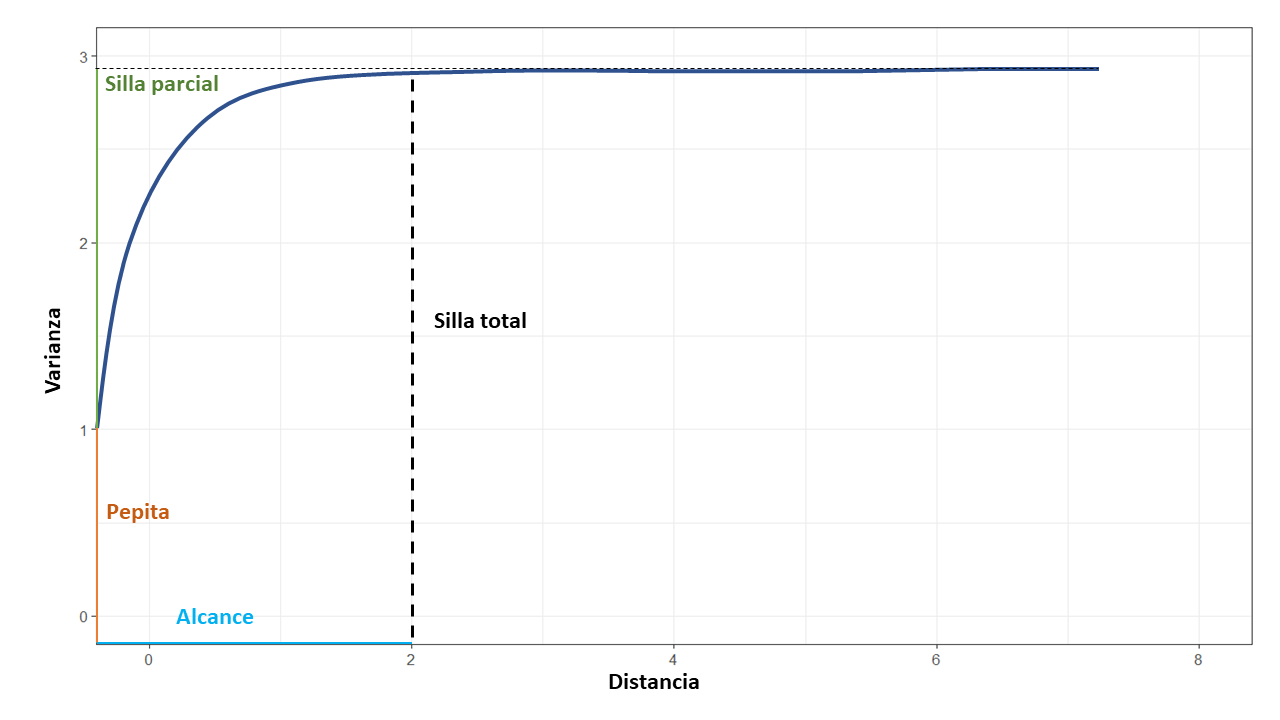
\includegraphics[width=17.78in]{figuras/otros/variograma_partes} \caption{Partes de un variograma}\label{fig:pvar}
\end{figure}

\hypertarget{variograma}{%
\section{Variograma}\label{variograma}}

En la práctica, se trabaja con las realizaciones del proceso estocástico o campo aleatorio en estudio; es decir, se cuenta con un conjunto de datos georeferenciados en un dominio dado. Utilizando estos datos, se puede inferir la estructura de dependencia espacial del fenómeno (\protect\hyperlink{ref-montero}{\textbf{montero?}}).

Por lo general, la descripción de la distribución espacial se limita a los primeros momentos. La esperanza o el momento de primer orden involucra un solo sitio a la vez y no proporciona información sobre la dependencia espacial. Por otro lado, la covarianza, correlograma y variograma o momentos de segundo orden están definidos mediante un par ubicaciones; así, estos momentos proporcionan información de la continuidad y dependencia espacial de la variable regionalizada (\protect\hyperlink{ref-emery}{\textbf{emery?}}).

\hypertarget{disimilitud-contra-separaciuxf3n}{%
\subsection{Disimilitud contra Separación}\label{disimilitud-contra-separaciuxf3n}}

La variabilidad de una variable regionalizada \(Z(s)\), se mide en diferentes escalas y se calcula a través de la disimilitud entre los valores \(z_{s1}\) y \(z_{s2}\) ubicados en los puntos \(s_1\) y \(s_2\) del domino espacial \(D\). La medida de disimilitud \(\hat{\gamma}\) de estos valores está dada por:

\begin{align}
  \hat{\gamma}(s_1,s_2)=\frac{(z_{s1}-z_{s2})^2}{2}  
\end{align}

Los dos puntos \(s_1\) y \(s_2\) en el espacio geográfico pueden unirse por un vector \(\textbf{h}=s_1-s_2\) como se muestra en la Figura \ref{fig:distanciah}.

\begin{figure}
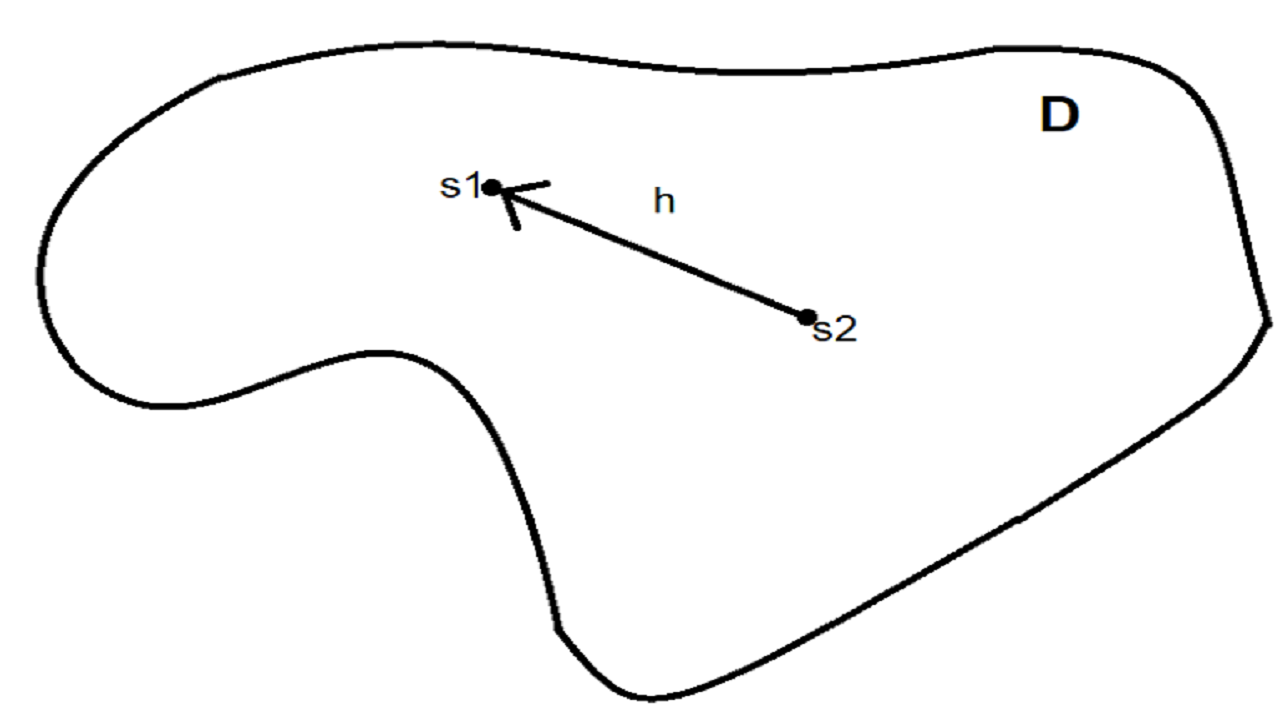
\includegraphics[width=17.78in]{figuras/otros/distancia_h} \caption{Distancia}\label{fig:distanciah}
\end{figure}

Si \(\hat{\gamma}\) es dependiente de la separación y orientación del par de ubicaciones descritos por el vector \(\textbf{h}\), se tiene que (\protect\hyperlink{ref-hans}{\textbf{hans?}}):

\begin{align}
  \hat{\gamma}(h)=\frac{1}{2}(z(s_1+\textbf{h})-z(s_1))^2  
\end{align}

La disimilitud es simétrica con respecto de \(h\), pues es una cantidad al cuadrado, por lo que, su representación será mostrada utilizando todos los pares de datos de la muestra en el conjunto \(D\). El gráfico de la disimilitud \(\hat{\gamma}\) contra la separación espacial absoluta \(h\), es llamado nube del variograma (\protect\hyperlink{ref-hans}{\textbf{hans?}}).

La disimilitud con frecuencia se incrementa con la distancia, pues los puntos cercanos tienden a ser similares (\protect\hyperlink{ref-hans}{\textbf{hans?}}) (ver Figura \ref{fig:varcloud} ).

\begin{figure}
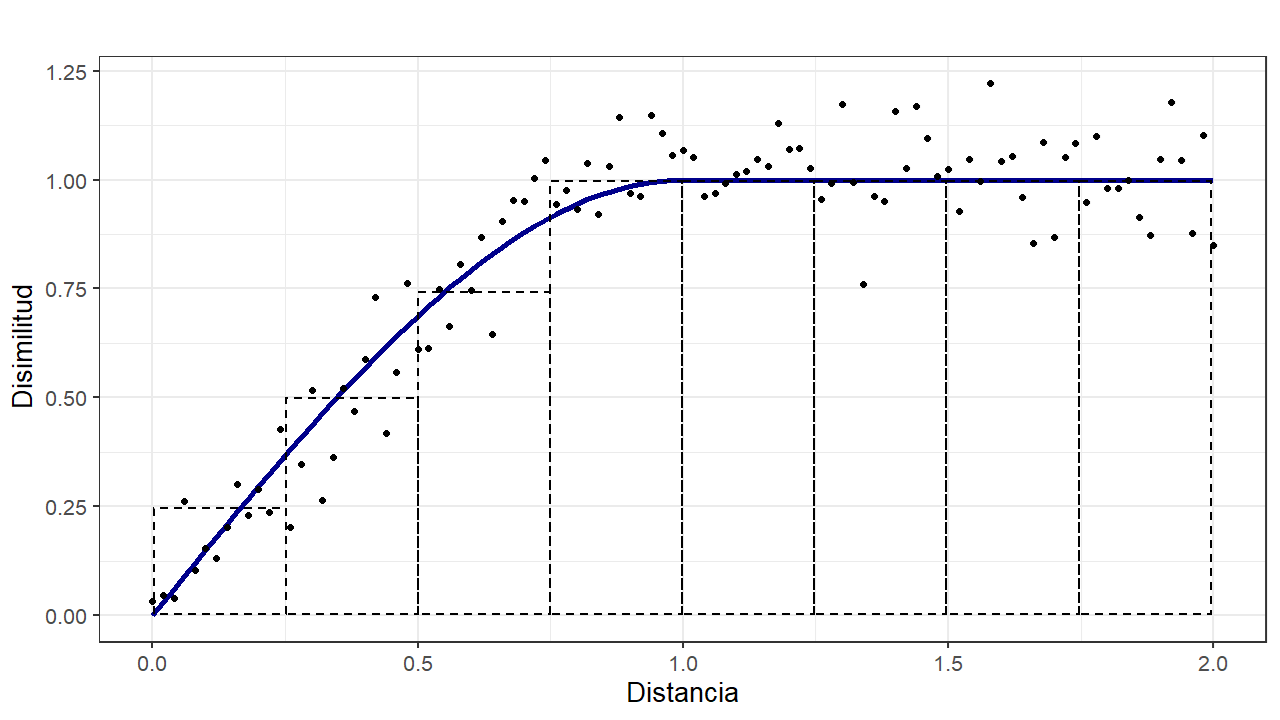
\includegraphics[width=17.78in]{figuras/otros/var_cloud} \caption{Disimilitud respecto de h.}\label{fig:varcloud}
\end{figure}

\hypertarget{variograma-empuxedrico}{%
\subsection{Variograma Empírico}\label{variograma-empuxedrico}}

Teniendo en cuenta que el variograma \(\gamma(\textbf{h})\) es la varianza de la variable de incrementos \(Z(s+\textbf{h})-Z(s)\), el estimador clásico se basa en la estimación de esta varianza mediante el método de momentos y está definido para un vector de separación \(\textbf{h}\) de la siguiente manera:

\begin{align}
  \hat{\gamma}(\textbf{h})=\frac{1}{2|N(\textbf{h})|}\sum_{N(\textbf{h})}(Z(s+\textbf{h})-Z(s))^2, \ \textbf{h}\in \mathbb{R}^d  
\end{align}

donde:

\begin{align}
  N(\textbf{h})=\{(s_i,s_j):s_i-s_j=\textbf{h}, i,j=1,...,n\}  
\end{align}

siendo \(N(\textbf{h})\) el conjunto de todos los pares de ubicaciones cuya separación corresponde a un vector \(\textbf{h}\) y \(|N(\textbf{h})|\) es la cardinalidad de \(N(\textbf{h})\). Nótese que \(N(-\textbf{h})\neq N(\textbf{h})\), aunque \(\hat{\gamma}(-\textbf{h})=\hat{\gamma}(\textbf{h})\), y la media \(\mu\) no necesita ser estimada.

Al ser un estimador de la varianza muestral es sensible a datos atípicos; es por ello que (\protect\hyperlink{ref-Cressi}{\textbf{Cressi?}}) propuso estimadores resistentes a datos atípicos, asumiendo normalidad marginal del campo aleatorio (\protect\hyperlink{ref-marta}{\textbf{marta?}}); sin embargo, la diferencia entre estos estimadores es pequeña (\protect\hyperlink{ref-Cressi}{\textbf{Cressi?}}).

\hypertarget{tolerancia-en-los-paruxe1metros-de-cuxe1lculo}{%
\subsubsection*{Tolerancia en los parámetros de cálculo}\label{tolerancia-en-los-paruxe1metros-de-cuxe1lculo}}
\addcontentsline{toc}{subsubsection}{Tolerancia en los parámetros de cálculo}

En la práctica, los datos están distribuidos irregularmente en el dominio espacial \(D\), por lo que el número de pares \(|N(\textbf{h})|\) que se utilizan en el cálculo del variograma empírico, \(\hat{\gamma}(\textbf{h})\) para un vector \(\textbf{h}\) dado, es por lo general escaso; dando como resultado una estimación del variograma empírico errónea, provocando que sea imposible de interpretarlo y modelarlo. Para corregir esto, se suelen añadir algunas tolerancias de cálculo sobre las distancias y direcciones, teniendo así que:

\begin{align}
  \hat{\gamma^+}(\textbf{h})=\frac{1}{2|N^+(\textbf{h})|}\sum_{N^+(\textbf{h})}(Z(s+\textbf{h})-Z(s))^2  
\end{align}

donde \(N^+=\{(s_i,s_j): s_i-s_j\in T(\textbf{h})\}=\displaystyle \bigcup_{\textbf{h}^{'}\in T(\textbf{h})}N(\textbf{h}')\)

Siendo \(T(\textbf{h})\) una región de tolerancia alrededor de \(\textbf{h}\); es decir, \(T(\textbf{h})=[\textbf{h}-\Delta \textbf{h},\textbf{h}+\Delta \textbf{h}]\) en el caso unidiminesional. En el caso de dimensión dos o tres, existen tolerancias sobre la longitud de \(\textbf{h}\) y sobre su orientación (\protect\hyperlink{ref-emery}{\textbf{emery?}}) (véase Figura \ref{fig:regtol}):

\begin{figure}
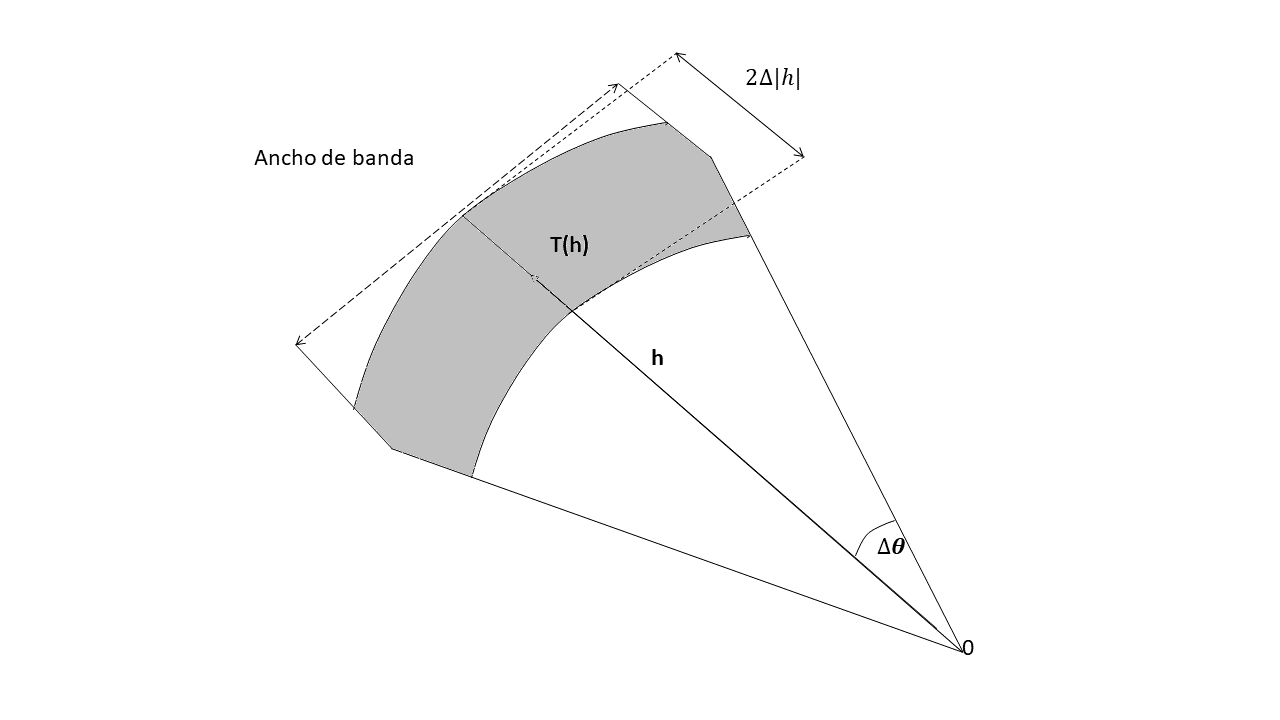
\includegraphics[width=17.78in]{figuras/otros/tolerancia} \caption{Región de tolerancia $T( extbf{h})$ alrededor del vector $   extbf{h}$}\label{fig:regtol}
\end{figure}

El ancho de banda limita la división del cono de tolerancia a una expansión máxima. En el espacio de tres dimensiones, se introducen dos anchos de banda, horizontal y vertical (\protect\hyperlink{ref-emery}{\textbf{emery?}}).

\hypertarget{propiedades-del-variograma-empuxedrico}{%
\subsubsection*{Propiedades del variograma empírico}\label{propiedades-del-variograma-empuxedrico}}
\addcontentsline{toc}{subsubsection}{Propiedades del variograma empírico}

\begin{itemize}
\item
  El variograma empírico \(\hat{\gamma}(\textbf{h})\) es un estimador insesgado del variograma teórico (\protect\hyperlink{ref-montero}{\textbf{montero?}}):

  \begin{align}
      E(\hat{\gamma}(\textbf{h}))=\gamma(\textbf{h})  
    \end{align}
\item
  La varianza relativa es un indicador de robustez:

  \begin{align}
      \frac{Var(\hat{\gamma}(\textbf{h}))}{(\gamma(\textbf{h}))^2}  
    \end{align}

  A medida que más alta sea dicha varianza, más susceptible es el variograma empírico de fluctuar en torno a su valor esperado, y más difícil se vuelve la inferencia estadística.

  Los principales factores que influyen en la varianza relativa son (\protect\hyperlink{ref-emery}{\textbf{emery?}}):

  \begin{itemize}
  \tightlist
  \item
    Norma del vector \(\textbf{h}\): la varianza relativa crece cuando la distancia aumenta.
  \item
    La irregularidad de la malla de muestreo, tiene la posibilidad de causar grandes variaciones en el cálculo del variograma empírico, incluso a distancias pequeñas.
  \item
    A medida que más reducido es el número de pares de datos, más grandes son las variaciones.
  \item
    La existencia de datos atípicos, puesto que en el cálculo del variograma empírico, se elevan los valores al cuadrado.
  \end{itemize}
\item
  Las direcciones de cálculo del variograma empírico deben tener en consideración la anisotropía de la variable regionalizada; en la situación de isotropía, donde los variogramas direccionales son semejantes, se puede tener en cuenta un variograma omnidireccional, determinado por:

  \begin{align}
      \bar{\gamma}^+(h)=\frac{1}{2|N^+(\textbf{h})|}\sum_{N^+(\textbf{h})}(Z(s+\textbf{h})-Z(s))^2  
    \end{align}

  donde: \(|N^+(\textbf{h})|=\{(s_i,s_j): s_i-s_j \thickapprox \textbf{h}\}\) (\protect\hyperlink{ref-montero}{\textbf{montero?}}).
\item
  Si el variograma presenta comportamiento anisotrópico es necesario realizar transformaciones de las coordenadas que permitan obtener variables regionalizadas anistrópicas a partir de los modelos isotrópicos (\protect\hyperlink{ref-hans}{\textbf{hans?}}).
\end{itemize}

\hypertarget{nube-variogruxe1fica}{%
\subsubsection*{Nube variográfica}\label{nube-variogruxe1fica}}
\addcontentsline{toc}{subsubsection}{Nube variográfica}

Teniendo presente que bajo el supuesto de estacionariedad, los valores \(\hat{\gamma}(s_i,s_j)\) son estimadores insesgados de los valores que corresponden \(\gamma(s_i,s_j)\). La recopilación de pares de distancias y sus correspondientes valores de variograma, \(\{(\textbf{h},\gamma(\textbf{h})): \textbf{h}=s_i-s_j\}\), es conocido como variograma empírico y su gráfico como nube variográfica. Para mejorar la conducta del variograma empírico como un estimador del variograma teórico \(\gamma(\textbf{h})\) es necesario aplicar un tipo de suavización, puesto que se espera que la función \(\gamma(\textbf{h})\) varíe suavemente en función de \(\textbf{h}\), por lo cual se disminuye la varianza sin añadir sesgo llevando a cabo un promedio de los valores de \(\hat{\gamma}\) sobre rangos o \textit{bins} adecuados de distancia entre puntos \(s_i,s_j\) (\protect\hyperlink{ref-peter}{\textbf{peter?}}).

Si el diseño de muestreo es una grilla regular la suavización puede ser lograda sin introducir sesgo, simplemente promediando todos los valores \(\hat{\gamma}(\textbf{h})\) para cada \(\textbf{h}\) diferente. Sin embargo, si el diseño es irregular, para un rango de ancho \(m\) se define un variograma \(\gamma_k\), para un entero positivo \(k\), como el promedio de todos los \(\hat{\gamma}(\textbf{h})\) para el cual la respectiva distancia \(h\) satisfaga \((k-1)m<h\leq km\); entonces, \(\gamma_k\) es aproximadamente una estimación insesgada de \(\gamma(h_k)\); por conveniencia se adopta \(h_k=(k-0.5)m\), que es el punto medio del intervalo respectivo (\protect\hyperlink{ref-peter}{\textbf{peter?}}).

\begin{figure}
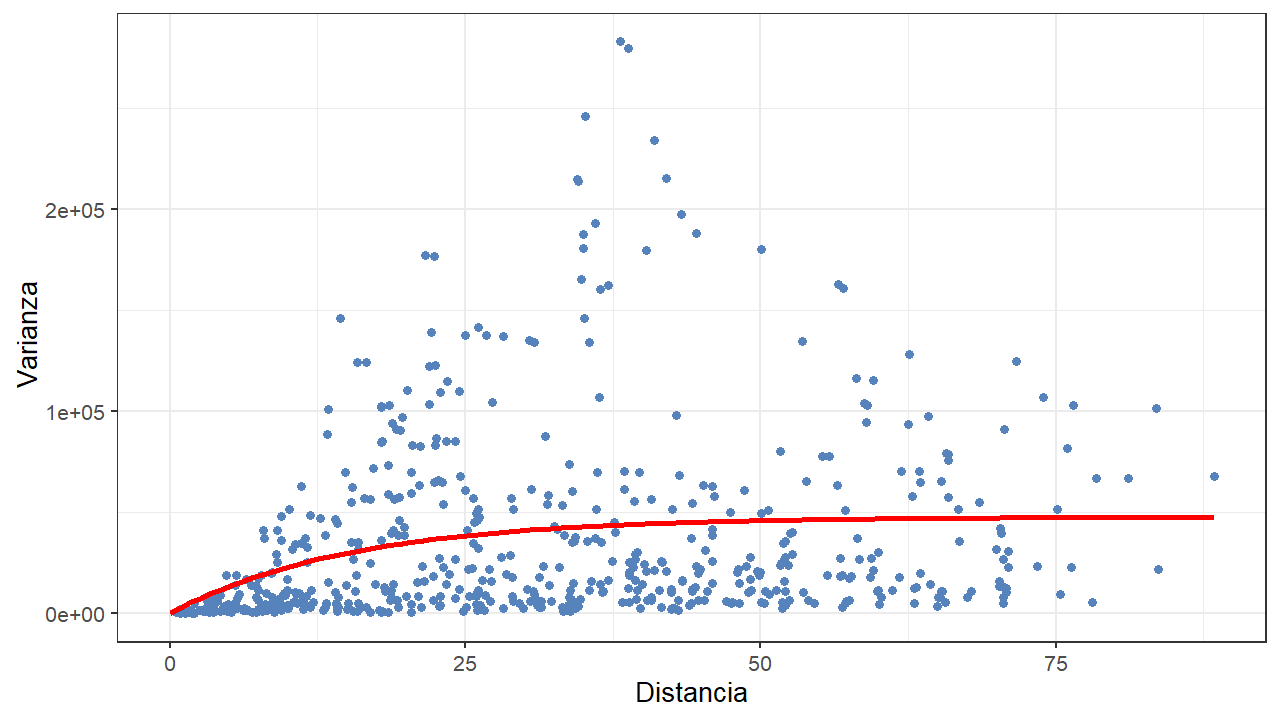
\includegraphics[width=17.78in]{figuras/otros/cloud_variogram} \caption{Nube variográfica}\label{fig:varcloud1}
\end{figure}
\begin{figure}
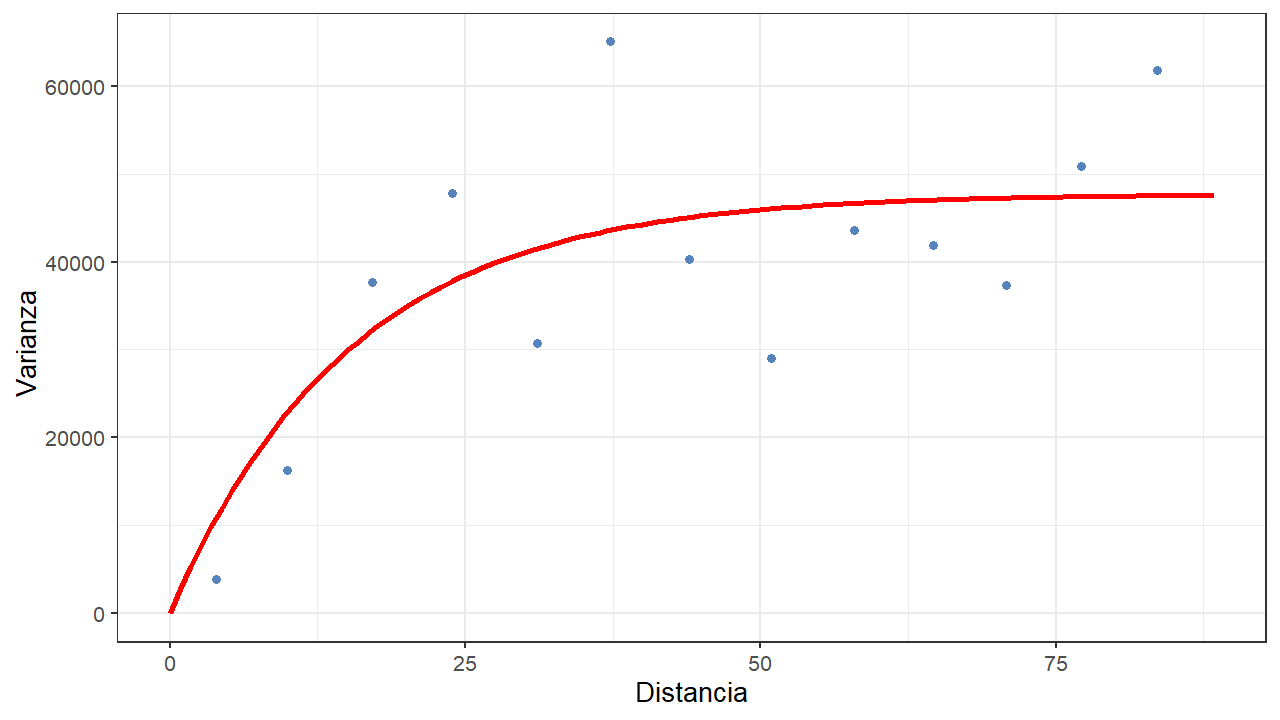
\includegraphics[width=17.78in]{figuras/otros/bin_variogram} \caption{Bin variograma}\label{fig:varcloud2}
\end{figure}

\hypertarget{estimaciuxf3n-del-variograma-ejemplos}{%
\subsection{Estimación del variograma (Ejemplos)*}\label{estimaciuxf3n-del-variograma-ejemplos}}

Se sabe que no se puede utilizar de manera directa el variograma emprírico, puesto que está definido para ciertas distancias y direcciones. Por otro lado, debido a los parámetros de tolerancia, está sujeto a aproximaciones, puesto que en el proceso de cálculo se utiliza un número limitado de datos. Para dar solución a esto, se ajusta un modelo teórico de variograma a partir del variograma empírico, siendo esta etapa la más significativa de todo análisis geoestadístico, puesto que nos da información de la continuidad espacial de la variable en estudio (\protect\hyperlink{ref-emery}{\textbf{emery?}}).

Una función de variograma teórico es ajustada a la sucesión de disimilitudes medias; nótese que este ajuste involucra una interpretación del comportamiento en el origen y el comportamiento para largas distancias, más allá del rango del variograma empírico. El ajuste puede llevarse a cabo de manera empírica mediante criterio experto, puesto que en la mayoría de casos prácticos no es fundamental el que tan bien la función de variograma se ajuste a la secuencia de puntos; lo más relevante es el tipo de continuidad que se asume para la variable regionalizada y la hipótesis de estacionariedad asociada al proceso estocástico espacial o campo aleatorio; estas suposiciones sirven de guía en la selección de una función de variograma teórico (\protect\hyperlink{ref-hans}{\textbf{hans?}}).

\hypertarget{comportamiento-en-el-origen}{%
\subsubsection*{Comportamiento en el origen}\label{comportamiento-en-el-origen}}
\addcontentsline{toc}{subsubsection}{Comportamiento en el origen}

Si las distancias son cercanas a cero; es decir, la variable regionalizada es regular en el espacio, más regular será el variograma en el origen. Generalmente, se suelen diferenciar tres tipos de comportamiento para el variograma en el origen (ver Figura \ref{fig:varcomp}) (\protect\hyperlink{ref-emery}{\textbf{emery?}}):

\begin{itemize}
\item
  Parabólico: Corresponde a una variable regionalizada bastante regular en el espacio.
\item
  Lineal: Corresponde a una variable regionalizada continua, pero no tan regular.
\item
  Discontinuo: Corresponde a una variable regionalizada más errática; es decir, con discontinuidades en la distribución espacial de sus valores. La diferencia entre dos datos bastante cercanos es grande, lo que provoca el efecto pepita.
\end{itemize}

\begin{figure}
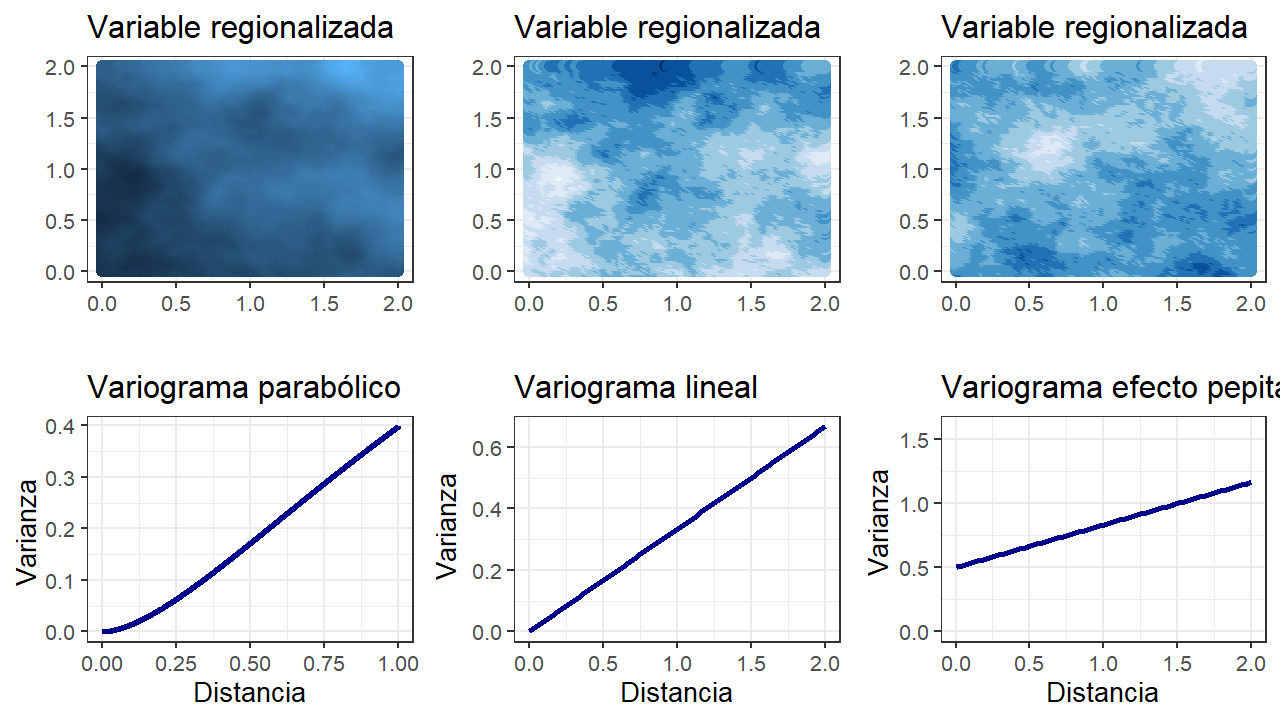
\includegraphics[width=17.78in]{figuras/otros/var_comp} \caption{Comportamientos del variograma en el origen.}\label{fig:varcomp}
\end{figure}

\hypertarget{comportamiento-para-distancias-muy-grades}{%
\subsubsection*{Comportamiento para distancias muy grades}\label{comportamiento-para-distancias-muy-grades}}
\addcontentsline{toc}{subsubsection}{Comportamiento para distancias muy grades}

El variograma habitualmente crece a partir del origen y se estabiliza a partir de una distancia \(\phi\), alrededor de una silla \(\sigma^2\); en este caso se conoce que esa silla es igual a la varianza a priori \(C(0)=\sigma^2\).

Como se vio anteriormente, las variables aleatorias \(Z(s)\) y \(Z(s+\textbf{h})\) están correlacionadas, si la longitud del vector de separación \(\textbf{h}\) es inferior a la distancia \(\phi\) o alcance; más allá de \(|h|=\phi\), el variograma es constante e igual a su silla, y las variables \(Z(s)\) y \(Z(s+\textbf{h})\) son independientes. Los variogramas con silla, se denominan \textit{modelos de transición} (ver Figura \ref{fig:varsill}) (\protect\hyperlink{ref-emery}{\textbf{emery?}}).

\begin{figure}
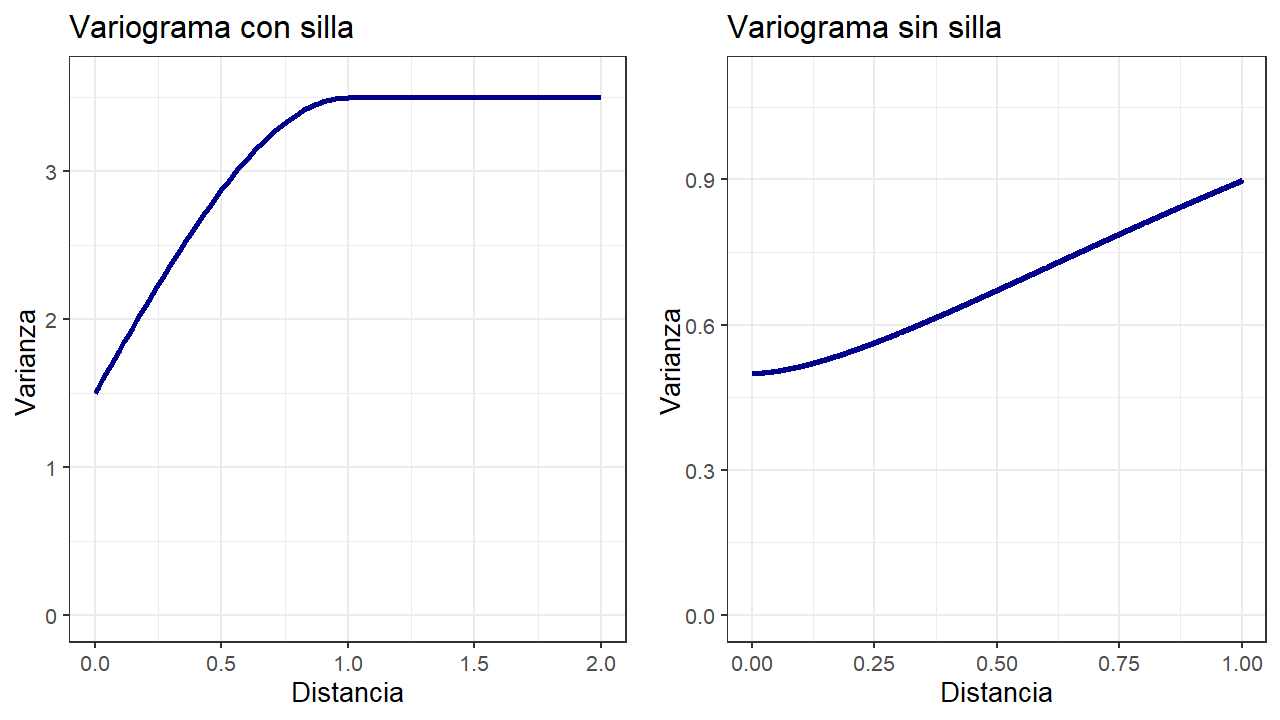
\includegraphics[width=17.78in]{figuras/otros/vari_sill} \caption{Lado izquierdo: Variograma con silla y alcance. Lado derecho: Variograma sin silla y  alcance.}\label{fig:varsill}
\end{figure}

Existen casos en los cuales el variograma crece infinitamente una vez la distancia se incrementa y no posee ni silla ni rango; en este caso, la varianza es infinita \(C(0)=\infty\) y no existe la función de covarianza ni el correlograma. Cuando se tiene ausencia de silla, es posible que sea una consecuencia del efecto de micro-escala (\protect\hyperlink{ref-emery}{\textbf{emery?}}).

\hypertarget{criterios-para-la-estimaciuxf3n-y-ajuste-del-variograma}{%
\subsection{Criterios para la estimación y ajuste del variograma}\label{criterios-para-la-estimaciuxf3n-y-ajuste-del-variograma}}

\hypertarget{tendencia}{%
\subsubsection*{Tendencia:}\label{tendencia}}
\addcontentsline{toc}{subsubsection}{Tendencia:}

Es fundamental verificar que los datos no presenten tendencia, puesto que cuando la media del proceso \(\mu(s)\) no es constante; es decir, el proceso no es estacionario, el variograma empírico calculado a partir de las observaciones es erróneo; este comportamiento de tendencia se puede comprobar mediante un gráfico de dispersión de la variable de respuesta frente a cada coordenada espacial (ver Figura \ref{fig:coordtrend}). En caso de que se evidencie tendencia se sugiere que se incluya un modelo de superficie de tendencia para la media que varía espacialmente, cuando una superficie de tendencia es incluida en el modelo, las dos coordenadas espaciales deben contribuir en este, puesto que la orientación de la región de estudio es arbitraria. En la práctica; al trabajar con datos geográficos de gran escala, se puede esperar que ciertas variables relacionadas a un ambiente físico muestren dependencia en la latitud (\protect\hyperlink{ref-peter}{\textbf{peter?}}).

\begin{figure}
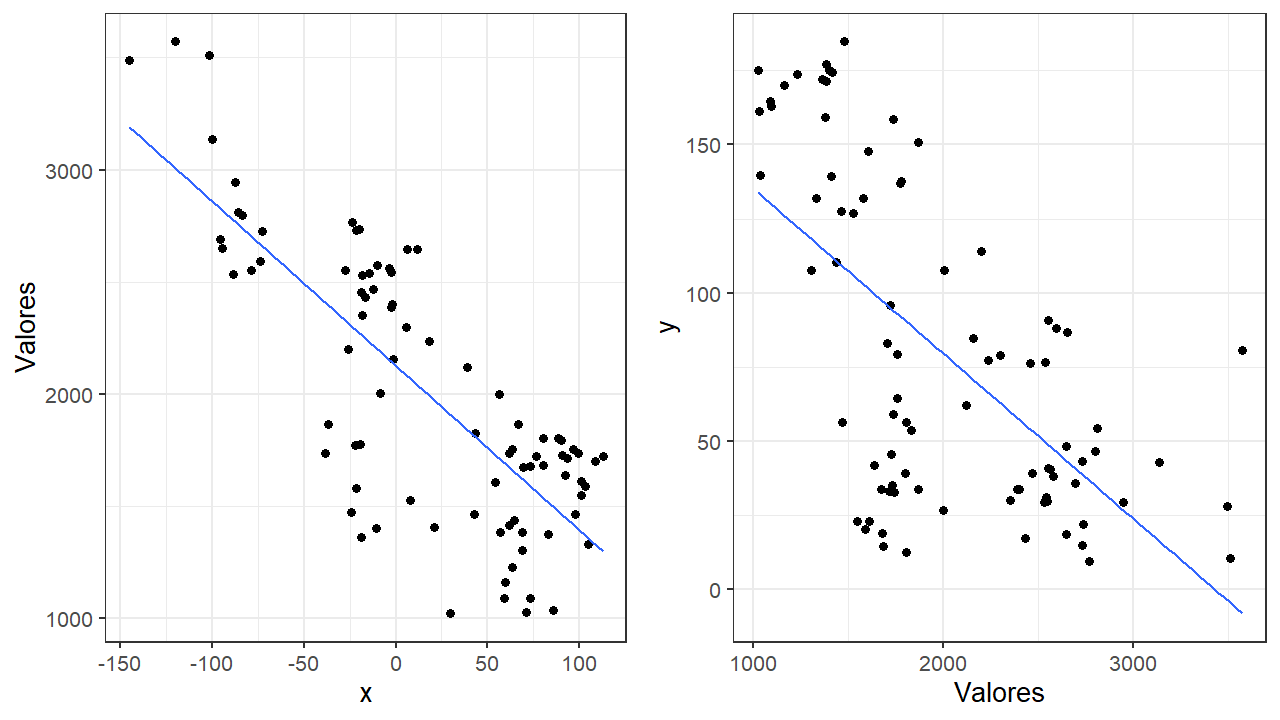
\includegraphics[width=17.78in]{figuras/otros/coord_trend} \caption{Tendencia}\label{fig:coordtrend}
\end{figure}

Cuando la función de media no es constante, el variograma empírico atribuye de manera errónea la variación inducida por esta a la estructura de convarianza de gran escala en el proceso no observado \(Z(s)\). Una solución es estimar \(\mu(s)\) mediante un modelo de superficie de tendencia o, si la información de la covariable está disponible, mediante un modelo general de regresión, y utilizar los residuos \(R_i=Z_i-\hat{\mu}(s_i)\) en lugar de las observaciones para el cálculo del variograma empírico (\protect\hyperlink{ref-peter}{\textbf{peter?}}). Este comportamiento se puede visualizar en la Figura \ref{fig:rcoordtrend}.

\begin{figure}
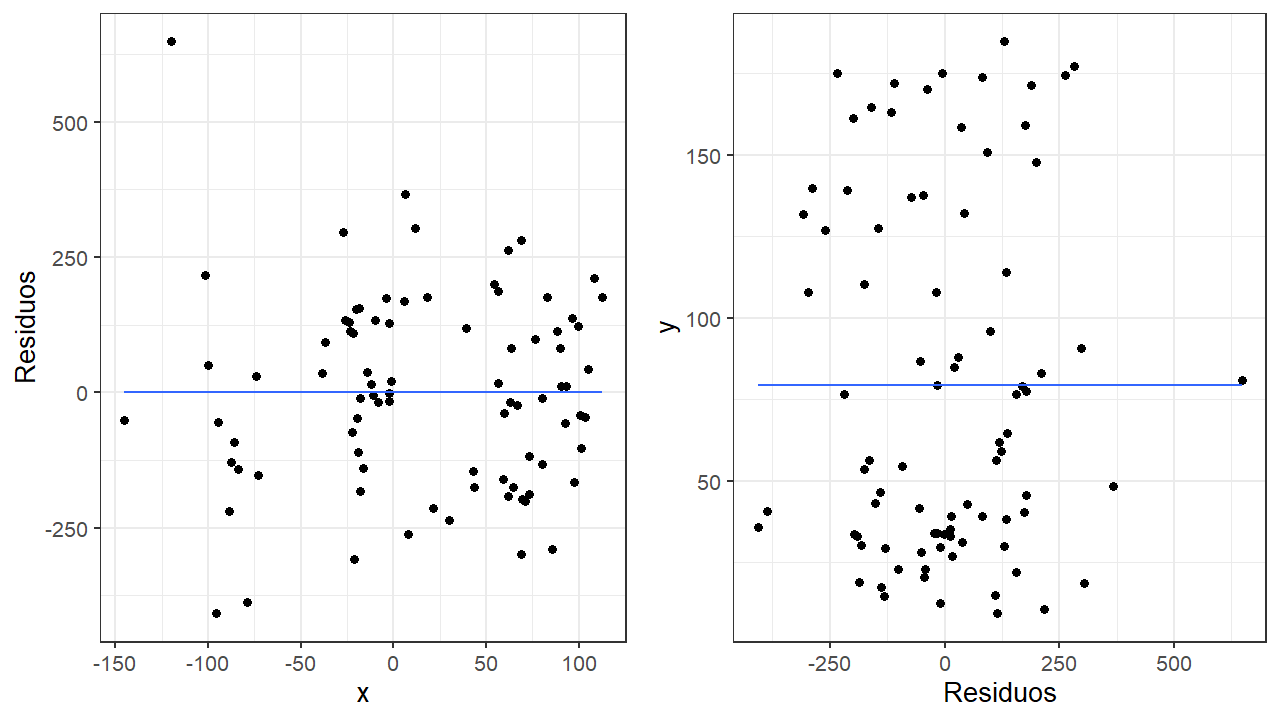
\includegraphics[width=17.78in]{figuras/otros/rcoord_trend} \caption{Tendencia}\label{fig:rcoordtrend}
\end{figure}

\hypertarget{establecer-la-variable-correcta}{%
\subsubsection*{Establecer la variable correcta:}\label{establecer-la-variable-correcta}}
\addcontentsline{toc}{subsubsection}{Establecer la variable correcta:}

En la estimación del variograma influye la distribución de los datos, pues estos pueden estar sesgados o tener valores extremos altos o bajos y por tanto su variograma calculado suele presentar un comportamiento errático. Para abordar este problema es recomendable transformar los datos a un espacio Normal o Gaussiano (\protect\hyperlink{ref-garten}{\textbf{garten?}}). Ver Figura \ref{fig:denvar}.

\begin{figure}
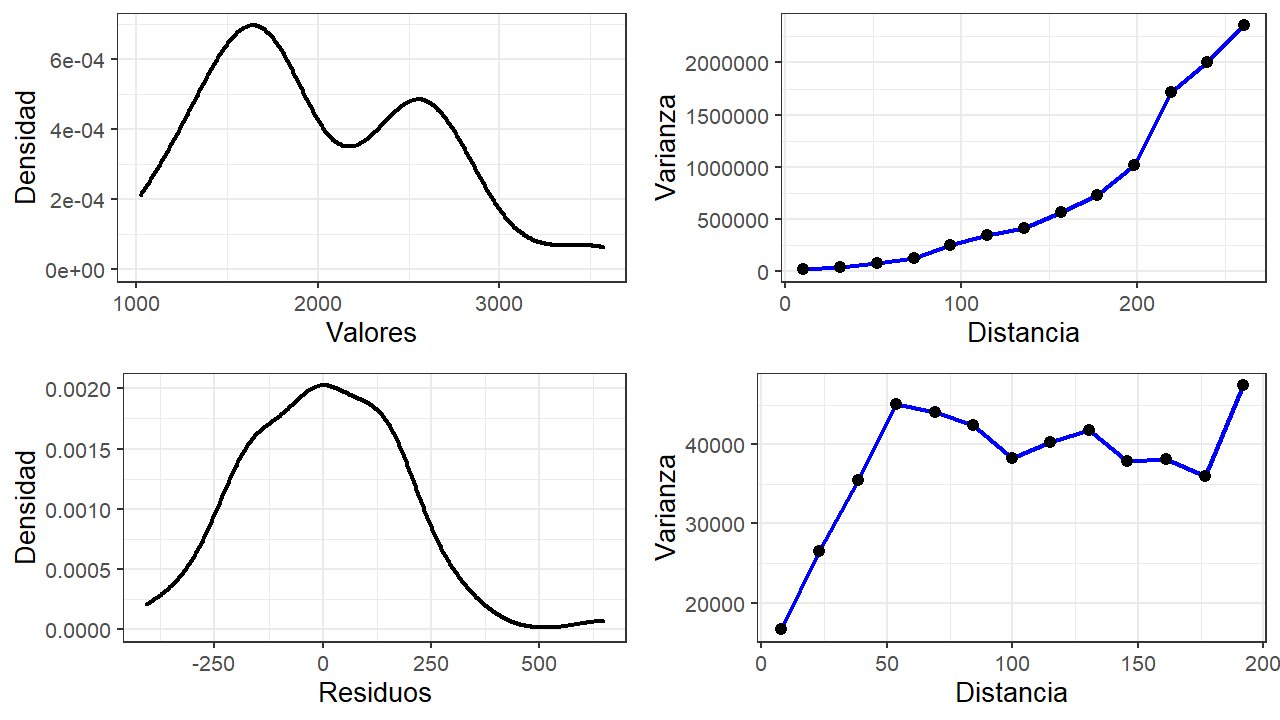
\includegraphics[width=17.78in]{figuras/otros/den_var} \caption{Arriba: Variograma empírico calculado a partir de los datos originales. Abajo: Variograma empírico calculado a partir de los residuos.}\label{fig:denvar}
\end{figure}

\hypertarget{verificaciuxf3n-de-isotropuxeda}{%
\subsubsection*{Verificación de isotropía:}\label{verificaciuxf3n-de-isotropuxeda}}
\addcontentsline{toc}{subsubsection}{Verificación de isotropía:}

Como bien se conoce, se debe verificar la estacionariedad de los datos, puesto que este influye de manera directa en la estimación del variograma empírico; teniendo en cuenta que un proceso espacial puede estar definido en varias direcciones, este criterio se debe verificar para todas estas. No obstante, en la práctica la isotropía se estudia por medio del cálculo de funciones de autocovariaza o de semivarianza muestrales en algunas direcciones que habitualmente son: \(0^o,45^o, 90^o\) y \(135^o\), ver Figura. \ref{fig:isodir}.

\begin{figure}
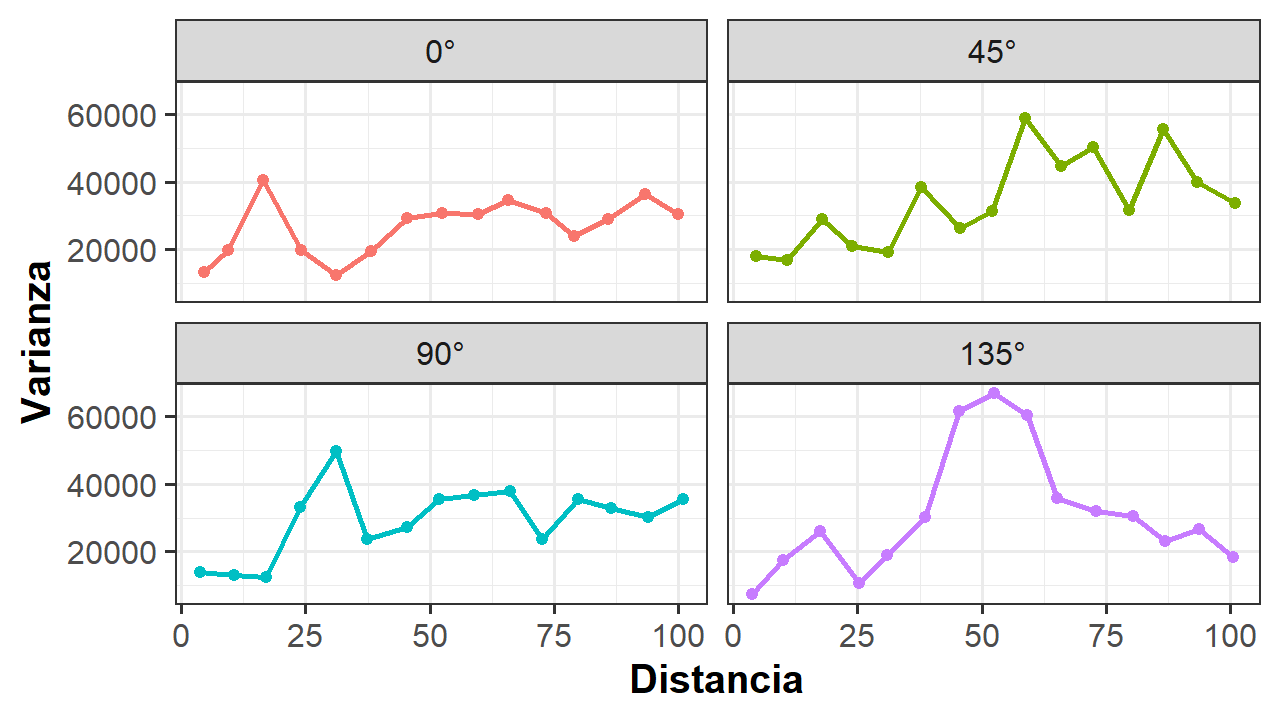
\includegraphics[width=17.78in]{figuras/otros/iso_dir} \caption{Comportamiento}\label{fig:isodir}
\end{figure}

Con la verificación de los puntos anteriores, se procede al cálculo del variograma empírico y su posterior ajuste de un modelo teórico por medio de los métodos que se exponen a continuación.

\hypertarget{muxe9todos-de-estimaciuxf3n-teuxf3rica-muxe1s-utilizados}{%
\subsection{Métodos de estimación teórica más utilizados}\label{muxe9todos-de-estimaciuxf3n-teuxf3rica-muxe1s-utilizados}}

Los parámetros de la función de covarianza pueden ser estimados por medio de los métodos de Máxima Verosimilitud (ML) y Máxima Verosimilitud restringida (REML), los cuales requieren la especificación de la distribución del vector \(Z=(Z(s_1),...,Z(s_n))\); generalmente, se asume normalidad multivariada. Para el caso ML, se tiene que:

\begin{align}
  Z\sim N_n(X\beta,\Sigma(\theta))  
\end{align}

donde \(\Sigma(\theta)=Cov(Z)\) es una matriz de dimensión \(n \times n\) y \(X\) es una matriz de dimensión \(n\times q\) con \(q<n\), de variables explicativas, dentro de las cuales comúnmente se encuentran las coordenadas geográficas; de donde el negativo de la función de logverosimil es:

\begin{align}
   L(\beta,\theta)=\frac{n}{2}\log(2\pi)+\frac{1}{2} \log|\Sigma(\theta|)+\frac{1}{2}(Z-X\beta)'\Sigma^{-1}(\theta)(Z-X\beta) 
\end{align}

El elemento \(i,j\) de la matriz \(\Sigma(\theta)\) corresponde a la covarianza espacial entre las variables \(Z(s_i)\) y \(Z(s_j)\); esto es:

\begin{align}
  Cov(Z(s_i),Z(s_j);\theta))=C(s_i-s_j;\theta)=C(\textbf{h};\theta)  
\end{align}

El estimador \(\hat{\theta}\) es sesgado pero asintóticamente eficiente; no obstante, al trabajar con una muestra grande se debe tener en consideración que debido a su conducta iterativa, se realizarán grandes cantidades de operaciones computacionales debido al cálculo del determinante y de la inversa de la matriz de covarianza (\protect\hyperlink{ref-marta}{\textbf{marta?}}).

\hypertarget{estimador-reml}{%
\subsubsection*{Estimador REML}\label{estimador-reml}}
\addcontentsline{toc}{subsubsection}{Estimador REML}

El estimador REML es una modificación del estimador ML propuesto para disminuir el sesgo, el cual reemplaza la maximización de la verosimilitud del vector \(Z\), por la del vector \(A'Z\) tal que: \(E(A'Z)=0\), donde \(A\) es una matriz de dimensión \(n\ \text{x}\ (n-p)\), de rango columna completo.

Con esta modificación y dado que \begin{align}
  Var(A'Z)=A'\Sigma(\theta)A  
\end{align}

el negativo de la función de logverosímil queda:

\begin{align}
   L(\theta)=\frac{n}{2}\log(2\pi)+\frac{1}{2} \log|A'\Sigma(\theta) A|+\frac{1}{2}Z'(A'\Sigma(\theta) A)^{-1} A'Z 
\end{align}

Esta función es dependiente únicamente de \(\theta\); de esta manera este método no usa la modelización de la superficie de tendencia, sino que se basa directamente en un vector de incrementos de media 0. No obstante, pese a minimizar el sesgo en las estimaciones de \(\theta\), aun interviene un costo computacional elevado (\protect\hyperlink{ref-marta}{\textbf{marta?}}).

\hypertarget{verosimilitud-compuesta-cl}{%
\subsubsection*{Verosimilitud Compuesta (CL)}\label{verosimilitud-compuesta-cl}}
\addcontentsline{toc}{subsubsection}{Verosimilitud Compuesta (CL)}

El método CL que se utiliza para estimar \(\theta\), involucra la suma de componentes individuales de funciones logverosimilitud, correspondiente a las distribuciones marginales de las variables de interés. Por consiguiente, la distribución multivariada de \(Z\) no es necesaria, puesto que se basa en las distribuciones marginales \(f(Z(s_i);\theta)\) y se asume la existencia del gradiente y de la matriz Hessiana de \(f\).

Ahora bien, se suponen conocidas \(f(Z(s_i);\theta)\), excepto el parámetro \(\theta\); entonces:

\begin{align}
  \log(Z(s_i);\theta)=\ln(f(Z(s_i);\theta))  
\end{align}

es una función logverosímil y la función de verosimilitud compuesta está definida por:

\begin{align}
   CL(\theta)=\sum_{i=1}^{n} \log(Z(s_i);\theta)  
\end{align}

Al gradiente de CL, \(\nabla CL=CS(\theta)\), se le conoce como función de score compuesta.

Así, los valores estimados de \(\hat{\theta}\) se determinan resolviendo el siguiente sistema de ecuaciones:

\begin{align}
   CS(\theta)=\sum_{i=1}^{n} \nabla\log(Z(s_i);\theta)=0  
\end{align}

Una de las razones principales para usar las funciones de verosimilitudes marginales es que aunque al inicio no se cumpla el supuesto requerido, es posible aproximarse a este por medio de alguna transformación (\protect\hyperlink{ref-marta}{\textbf{marta?}}).

\hypertarget{muxednimos-cuadrados-ponderados}{%
\subsubsection*{Mínimos cuadrados ponderados}\label{muxednimos-cuadrados-ponderados}}
\addcontentsline{toc}{subsubsection}{Mínimos cuadrados ponderados}

Este método utiliza la matriz de ponderación \(W(\theta)\) y suele ser expresado en términos del variograma o de la covarianza, gracias a su equivalencia en procesos estacionarios de segundo orden. Para el caso espacio-temporal, se estima \(\theta\) para un variograma minimizando la siguiente expresión:

\begin{align}
  (2\hat{\gamma}-2\gamma(\theta))'W^{-1}(\theta)(2\hat{\gamma}-2\gamma(\theta))  
\end{align}

donde la matriz de ponderación \(W(\theta)\) está dada por:

\begin{align}
  W(\theta)=Diag(Var(2\hat{\gamma}(\textbf{h}_k)))\approx Diag\left(\frac{2(2\gamma(\textbf{h}_k|\theta))^2}{N(\textbf{h}_k)}\right)  
\end{align}

con:

\begin{align}
  N(\textbf{h}_k)=\{(i,j):s_i-s_j=\textbf{h}_k\}  
\end{align}

Para las ubicaciones \(i,j=1,...,n\), que producen los primeros \(k\) rezagos espaciales \(k=1,...,K\); generalmente se utilizan los rezagos espaciales hasta la mitad de la distancia máxima entre cualquier par de ubicaciones, debido a que para ubicaciones bastante separadas disminuye notoriamente la cantidad de puntos incluidos en la estimación del variograma. La aproximación de \(Var(2\hat{\gamma}(\textbf{h}_k|\theta))\), se obtiene bajo el supuesto de que \(Z(s)\sim N(\mu;\sigma^2), \forall s\in \mathbb{R}^d\), y que por consiguiente:

\begin{align}
  (Z(s+\textbf{h})-Z(s))^2\approx 2\gamma(\textbf{h})\chi_1^2   
\end{align}

El inconveniente que presenta este método es la necesidad de definir clases de rezagos para realizar una estimación empírica de la covarianza o del variograma, pues si no se poseen muchos datos la cantidad de estos en cada una de las clases disminuye, de tal forma que para los primeros rezagos se pueden tener suficientes datos para la estimación de cada \(\hat{\gamma}(\textbf{h}_k)\); sin embargo, para los últimos rezagos podrían no existir suficientes datos para la estimación (\protect\hyperlink{ref-marta}{\textbf{marta?}}).

\hypertarget{modelo-lineal-de-regionalizaciuxf3n}{%
\subsubsection*{Modelo lineal de regionalización}\label{modelo-lineal-de-regionalizaciuxf3n}}
\addcontentsline{toc}{subsubsection}{Modelo lineal de regionalización}

En la práctica, puede suceder que el variograma empírico no presente una apariencia o forma simple de ser modelizado por un modelo teórico; no obstante, esto no es un inconveniente, puesto que existe la posibilidad de combinar modelos teóricos de variograma, obteniendo nuevos modelos más complejos.

Teniendo presente que un fenómeno regionalizado podría ser considerado como la suma de diversos subfenómenos independientes, el modelo lineal de regionalización construye un campo aleatorio \(Z(s)\) como una combinación lineal de \(L\) campos aleatorios independientes, cada uno con media 0 y función de covarianza \(C_l(h)\), mutuamente independientes (\protect\hyperlink{ref-marta}{\textbf{marta?}}).

Así, sea \(Y_l\) un subcampo aleatorio de \(Z\) para todo \(l=1,...,L\), se tiene que:

\begin{align}
  Z(s)=\sum_{l=0}^{L}a_lY_l(s)+\mu
\end{align}

con:

\begin{align}
    E(Z(s))&=\mu\\
    E(Y_l(s))&=0\\
    Cov(Y_l(s),Y_{l'}(s+\textbf{h}))&= \left \{ \begin{matrix} C_l(h) & si \ l=l'
\\ 0 & en\ otro\ caso.
\end{matrix}\right.  
\end{align}

Esto implica que la función de covarianza de \(Z(s)\) es una combinación lineal de las \(L\) funciones \(C_l(h)\) y bajo el supuesto de independencia entre los \(Y\), se tiene que:

\begin{align}
    C(h)&=Cov(Z(s),Z(s+\textbf{h}))\\
    &= \sum_{l=0}^L\sum_{l'=0}^L Cov((Y_l(s),Y_{l'}(s+\textbf{h}))) \\
    &=\sum_{l=0}^La_la_lC_l(h)\\
    &=\sum_{l=0}^La_l^2C_l(h)
\end{align}

por lo tanto, el modelo de convarianza \(C(h)\) es:

\begin{align}
  C(h)=\sum_{l=0}^Lb_lC_l(h),\ con\ b_l=a_l^2\geq 0  
\end{align}

De esta forma, como \(b_l>0\) es siempre positivo, y es la silla del modelo básico de covarianza \(C_l(h)\). Las condiciones suficientes para que \(C(h)\) sea un modelo válido de covarianza son:

\begin{itemize}
\tightlist
\item
  Las funciones \(C_l(h)\) son modelos de convarianza válidos.
\item
  \(b_l>0,\ \forall_l=1,...,L\)
\end{itemize}

En términos de variogramas, se tiene que:

\begin{align}
  E\left[ (Y_l(s)-Y_l(s+\textbf{h}))(Y_{l'}(s)-Y_{l'}(s+\textbf{h}))  \right]=\left \{ \begin{matrix} \gamma'_l(h) & si\ l=l'\\ 
0 & en\ otro\ caso. 
\end{matrix}\right.    
\end{align}

Entonces,

\begin{align}
   \gamma(h)=\frac{1}{2} E[Z(s+\textbf{h})-Z(s)]^2=\sum_{l=0}^Lb_l\gamma'_l(h) 
\end{align}

con \(b_l=(a_l)^2\geq 0\), donde \(b_l\) es la contribución en varianza del correspondiente variograma \(\gamma'_l(h)\) (\protect\hyperlink{ref-marta}{\textbf{marta?}}).

\textbf{GRAFICOSY EJEMPLOS}

\hypertarget{modelos-teuxf3ricos-de-variograma}{%
\subsection{Modelos teóricos de variograma}\label{modelos-teuxf3ricos-de-variograma}}

En esta sección se presentan las funciones de variograma más comunes, que se definen para el caso isotrópico de funciones aleatorias. Para la representación gráfica de la función de variograma se hace uso de la relación \(\gamma(h)=C(0)-C(h)\). Estas funciones se pueden clasificar de la siguiente manera:

\begin{itemize}
\tightlist
\item
  Variogramas con silla o variogramas de transición.
\item
  Variogramas con silla y efecto hueco.
\item
  Variogramas sin silla.
\end{itemize}

\hypertarget{variogramas-con-silla}{%
\subsubsection*{Variogramas con silla}\label{variogramas-con-silla}}
\addcontentsline{toc}{subsubsection}{Variogramas con silla}

\textbf{Modelo esférico}

Este modelo es válido solo en \(\mathbb{R}^1,\mathbb{R}^2,\mathbb{R}^3\), y está definido por:

\begin{align}
    \gamma(||\textbf{h}||;\theta) = \left \{ \begin{matrix} \sigma^2\left(1.5\frac{||\textbf{h}||}{\phi}-0.5\left(\frac{||\textbf{h}||}{\phi}\right)^3 \right) &  si \ ||\textbf{h}||\leq \phi
\\ \sigma^2 &  si\ ||\textbf{h}||>\phi \end{matrix}\right. 
\end{align}

con \(\theta=(\sigma^2,\phi)\), donde \(\sigma^2=C(0)\) es el valor del variograma donde alcanza la silla, y \(\phi\) es el rango.\textbackslash{}

Este variograma presenta un comportamiento lineal cerca del origen, lo cual sugiere continuidad pero con cierto grado de irregularidad en el proceso estocástico espacial o campo aleatorio. Sin embargo, referente a su comportamiento en distancias largas, alcanza su silla en \(||\textbf{h}||=\phi\). El uso habitual de este modelo en la práctica es gracias a su rango bien definido, su representación polinomial simple y su validez en \(\mathbb{R}^1,\mathbb{R}^2,\mathbb{R}^3\). La principal razón para el uso de este es que se comporta de forma casi lineal hasta que alcanza su silla, y presenta estabilidad en una gran variedad de observaciones.

\begin{figure}
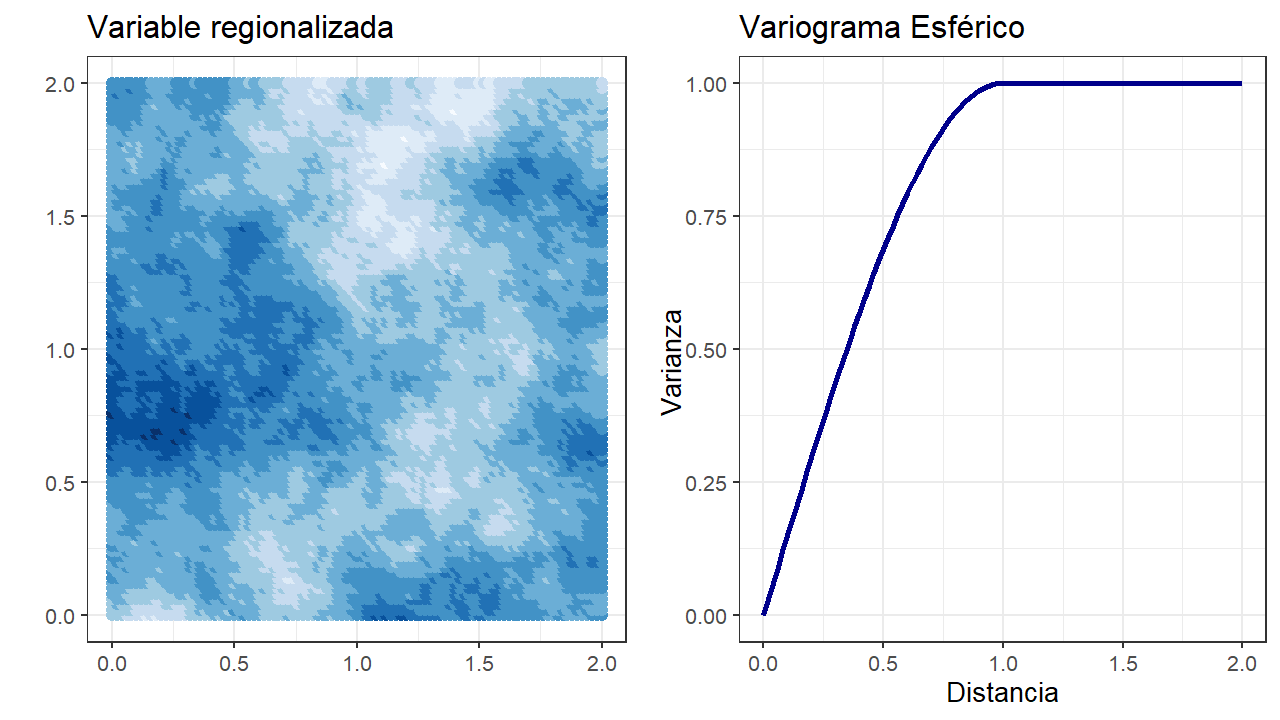
\includegraphics[width=17.78in]{figuras/otros/sph_var} \caption{Izquierda: Variable regionalizada. Derecha: Variograma esférico.}\label{fig:sphvar}
\end{figure}

\textbf{Modelo de efecto pepita puro}

Este variograma refleja la ausencia de dependencia espacial en el proceso estocástico o campo aleatorio; este modelo puede ser visto como un caso particular del modelo esférico si \(\phi \to 0\):

\begin{align}        
    \gamma(||\textbf{h}||;\theta) = \left \{ \begin{matrix} \sigma^2&  si \ ||\textbf{h}|| =0\\
    0 &  si\ ||\textbf{h}||>0 \end{matrix}\right.
    \end{align}

con \(\theta=\sigma^2\).

Se debe tener en cuenta que el modelo esférico corresponde a una función aleatoria continua, mientras que el modelo de efecto pepita puro, a una discontinuidad.

\begin{figure}
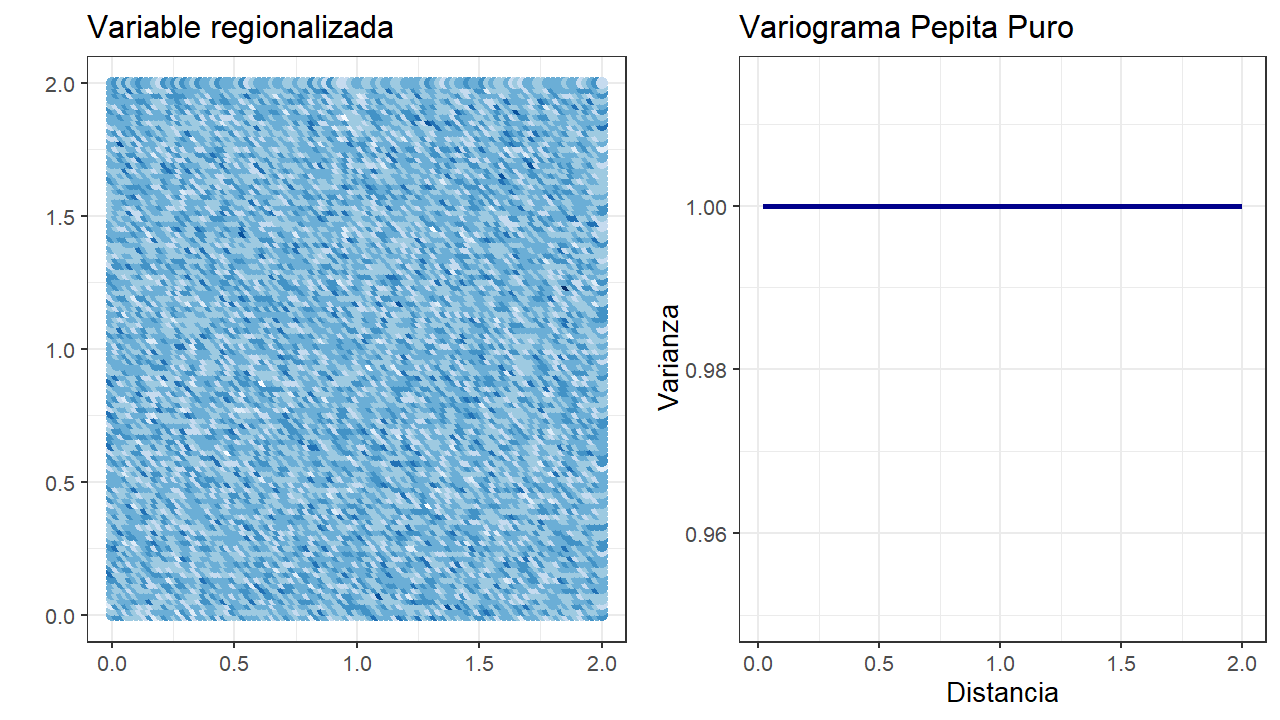
\includegraphics[width=17.78in]{figuras/otros/pepita_var} \caption{Izquierda: Variable regionalizada. Derecha: Variograma pepita puro.}\label{fig:unnamed-chunk-2}
\end{figure}

\textbf{Modelo exponencial}

Este modelo es válido en \(\mathbb{R}^d,\ d\geq 1\), y está definido por:

\begin{align}
    \gamma(||\textbf{h}||;\theta)=\sigma^2 \left(1-\exp\left(-\frac{||\textbf{h}||}{\phi}\right) \right),\quad \theta=(\sigma^2,\phi)
\end{align}

El modelo exponencial refleja un comportamiento lineal cerca del origen, lo cual indica continuidad pero con un cierto grado de irregularidad en la función aleatoria. Por otro lado, en cuanto a su comportamiento en largas distancias, este alcanza su silla solo asintóticamente cuando \(||\textbf{h}||\to \infty\). El valor del rango es igual a la distancia para el cual el variograma toma un valor igual al \(95\%\) de la silla.

\begin{figure}
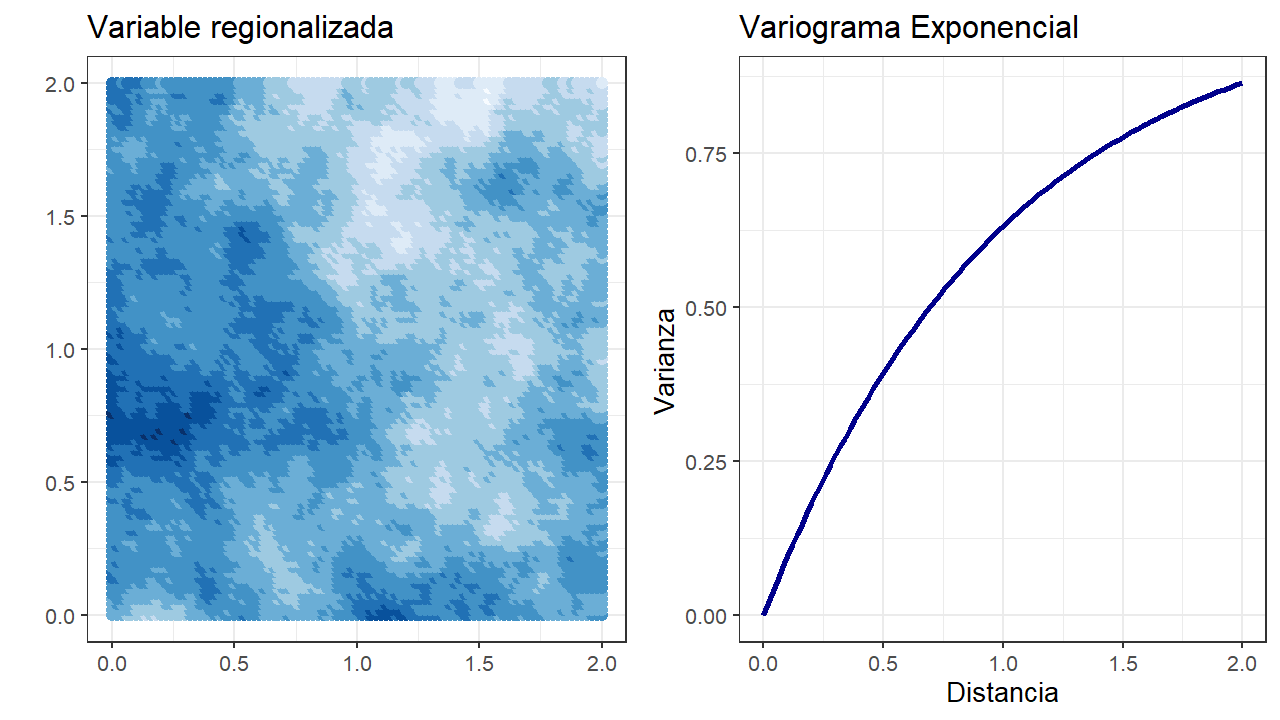
\includegraphics[width=17.78in]{figuras/otros/exp_var} \caption{Izquierda: Variable regionalizada. Derecha: Variograma exponencial.}\label{fig:unnamed-chunk-3}
\end{figure}

\textbf{Modelo Gaussiano}

Este modelo es válido en \(\mathbb{R}^d,\ d\geq 1\), y está definido por:

\begin{align}
    \gamma(||\textbf{h}||;\theta)=\sigma^2\left(1-\exp\left(-\frac{||\textbf{h}||^2}{\phi^2} \right) \right),\quad \theta=(\sigma^2,\phi)
\end{align}

La principal característica de este modelo es su forma parabólica cerca al origen; la dependencia espacial se desvanece solo en una distancia que tiende a infinito; por consiguiente, este modelo es considerado poco realista en la práctica.

\begin{figure}
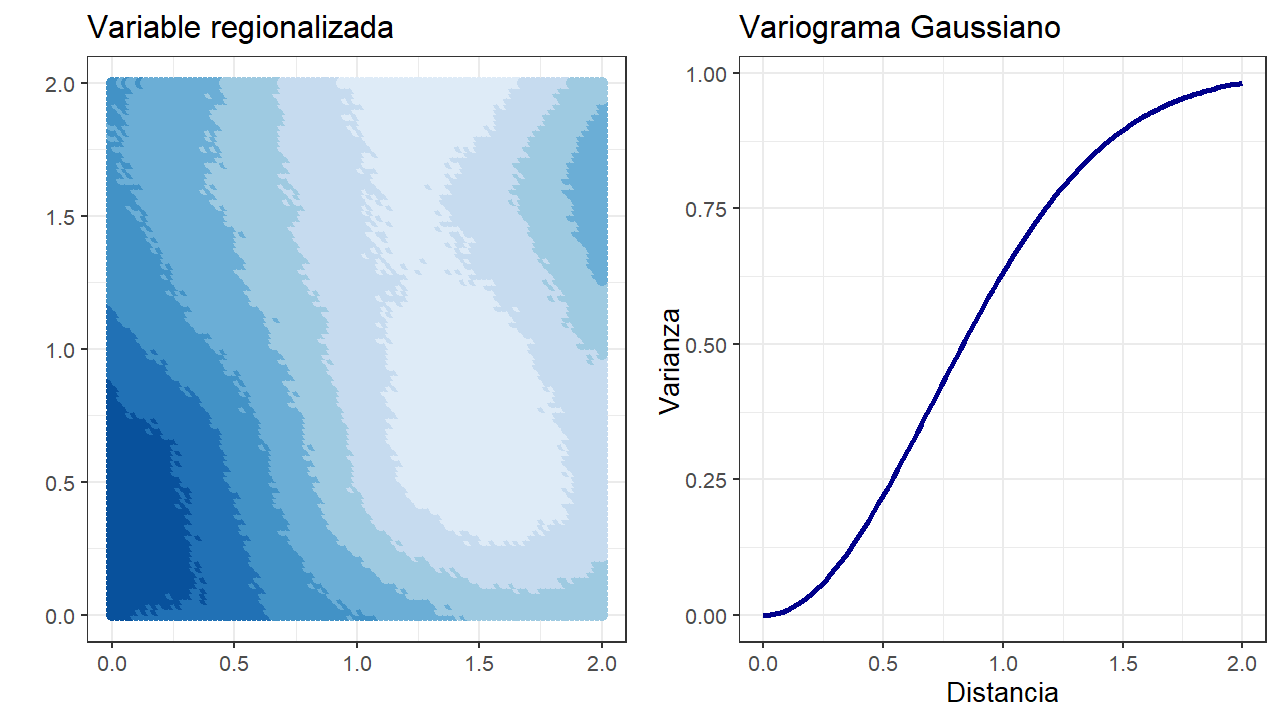
\includegraphics[width=17.78in]{figuras/otros/gau_var} \caption{Izquierda: Variable regionalizada. Derecha: Variograma Gaussiano.}\label{fig:gauvar}
\end{figure}

\textbf{Modelo Cúbico}

Este modelo es válido en \(\mathbb{R}^1,\mathbb{R}^2,\mathbb{R}^3\); generalmente es similar al modelo Gaussiano, puesto que también presenta un comportamiento parabólico cerca del origen. Sin embargo, este modelo alcanza una silla plana a una distancia \(\phi\), y esta definido por:

\begin{align}
    \gamma(||\textbf{h}||;\theta)=\left \{ \begin{matrix} \sigma^2\left(7\frac{||\textbf{h}||^2}{\phi^2}-\frac{35||\textbf{h}||^3}{4\phi^3}+\frac{7||\textbf{h}||^5}{2\phi^5}-\frac{3||\textbf{h}||^7}{4\phi^7} \right) &  si \ 0\leq||\textbf{h}||\leq\phi\\
    \sigma^2 &  si\ ||\textbf{h}||>\phi \end{matrix}\right.
\end{align}

con \(\theta=(\sigma^2,\phi)\).

\begin{figure}
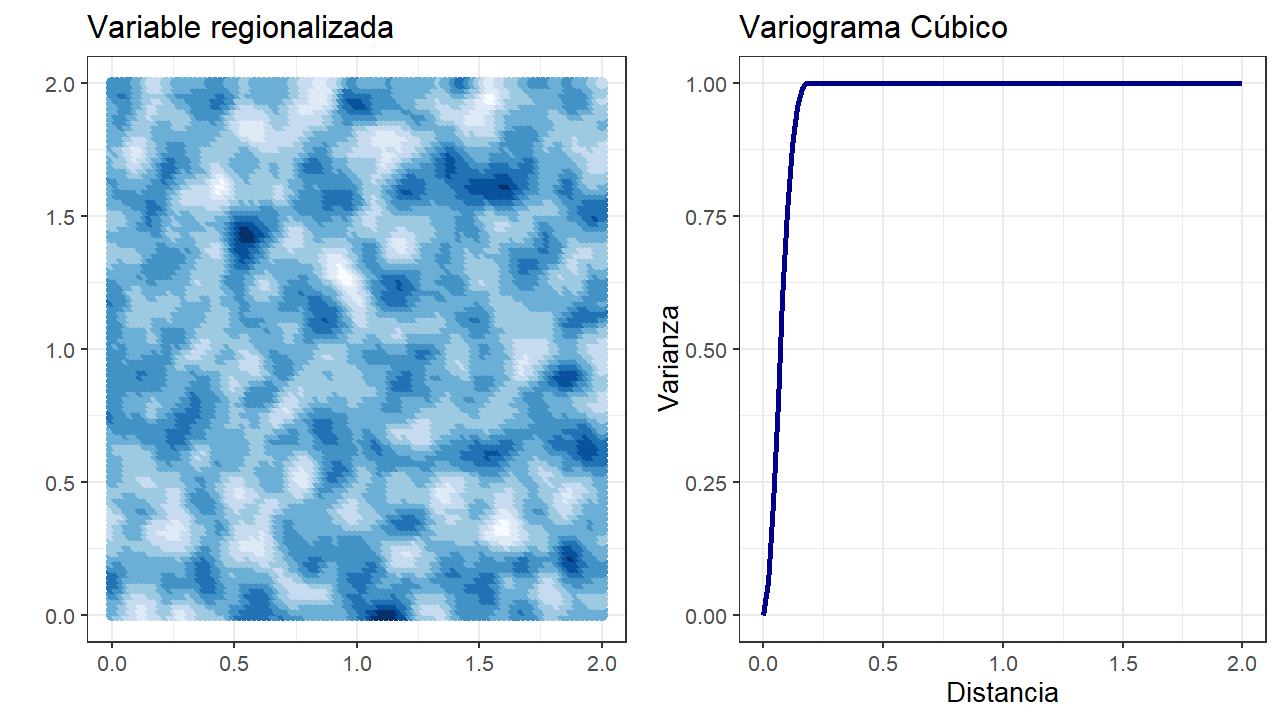
\includegraphics[width=17.78in]{figuras/otros/cub_var} \caption{Izquierda: Variable regionalizada. Derecha: Variograma cúbico.}\label{fig:cubvar}
\end{figure}

\textbf{Modelo Estable}

Este modelo es válido en \(\mathbb{R}^d,\ d\geq1\) y está definido por:

\begin{align}
    \gamma(||\textbf{h}||;\theta)=\sigma^2 \left(1-\exp\left(-\left(\frac{||\textbf{h}||}{\phi}\right)^\alpha\right) \right),\quad 0<\alpha \leq 2,\ \theta=(\sigma^2,\phi)
\end{align}

Notar que para \(\alpha=1\), se obtiene el modelo exponencial y con \(\alpha=2\), se convierte en un modelo Gaussiano.

\begin{figure}
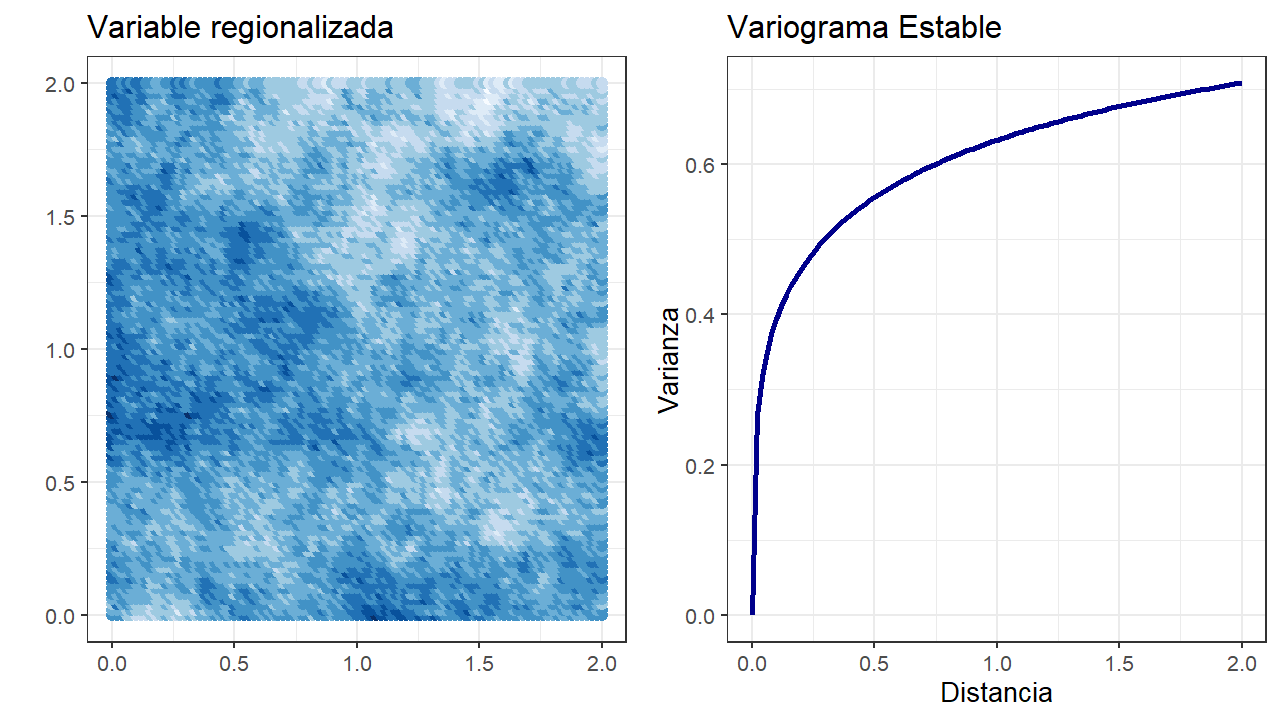
\includegraphics[width=17.78in]{figuras/otros/estable_var} \caption{Izquierda: Variable regionalizada. Derecha: Variograma estable.}\label{fig:establevar}
\end{figure}

\textbf{Modelo de Cauchy Generalizado}

Este modelo es válido en \(\mathbb{R}^d,\ d\geq1\), y está definido por:

\begin{align}
    \gamma(||\textbf{h}||;\theta)=\sigma^2\left(1-\frac{1}{\left(1+\left( \frac{||\textbf{h}||}{\phi} \right)^2\right)^\alpha} \right), \quad \theta=(\sigma^2,\phi)
\end{align}

Si \(\alpha=1\) es conocido como el modelo de Cauchy.

Este modelo muestra un comportamiento parabólico cerca del origen y si \(\alpha<2\) alcanza la silla lentamente.

\begin{figure}
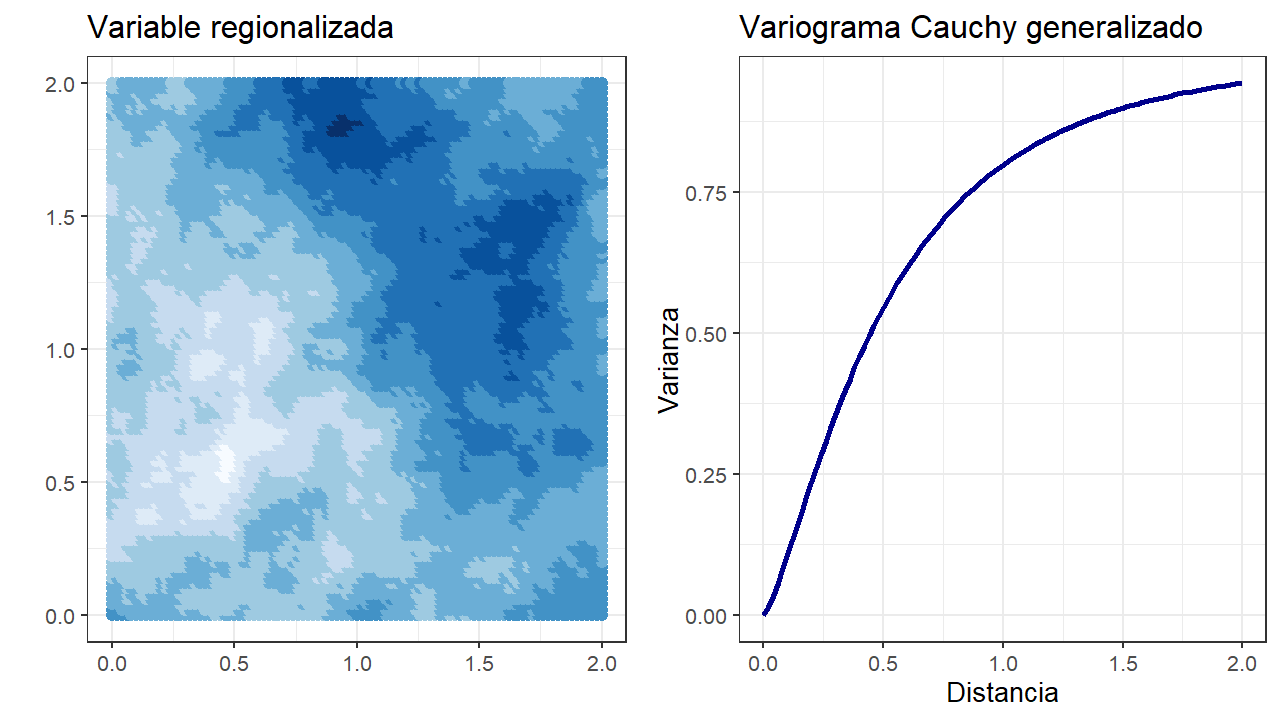
\includegraphics[width=17.78in]{figuras/otros/caugen_var} \caption{Izquierda: Variable regionalizada. Derecha: Variograma Cauchy generalizado.}\label{fig:caugenvar}
\end{figure}

\textbf{Modelo de K-Bessel o Matérn}

Este modelo es válido en \(\mathbb{R}^d,\quad d \geq 1\), y esta definido por:

\begin{align}
    \gamma(||\textbf{h}||;\theta)=\sigma^2\left(1-\frac{1}{2^{\alpha-1}\Gamma(\alpha)}\left(\frac{||\textbf{h}||}{\phi} \right)^\alpha K_\alpha \left(\frac{||\textbf{h}||}{\phi} \right) \right),\quad \alpha>0,\ \theta=(\sigma^2,\phi)
\end{align}

donde \(K_\alpha\) es la función de Bessel modificada de segundo tipo de orden \(\alpha\), y que está definida por:

\begin{align}
    K_\alpha (\nu) =\frac{\pi}{2\sin(\alpha \pi)}\left(\sum_{k=0}^\infty {\frac{1}{k!\Gamma(-\alpha+k+1)}\left(\frac{\nu}{2}\right)^{2k-\alpha}}-\sum_{k=0}^\infty {\frac{1}{k!\Gamma(\alpha+k+1)}\left(\frac{\nu}{2}\right)^{2k+\alpha}}\right)
\end{align}

El modelo K-Bessel puede tener cualquier tipo de comportamiento cerca del origen. Para \(\alpha=1/2\), se obtiene el modelo exponencial.

\begin{figure}
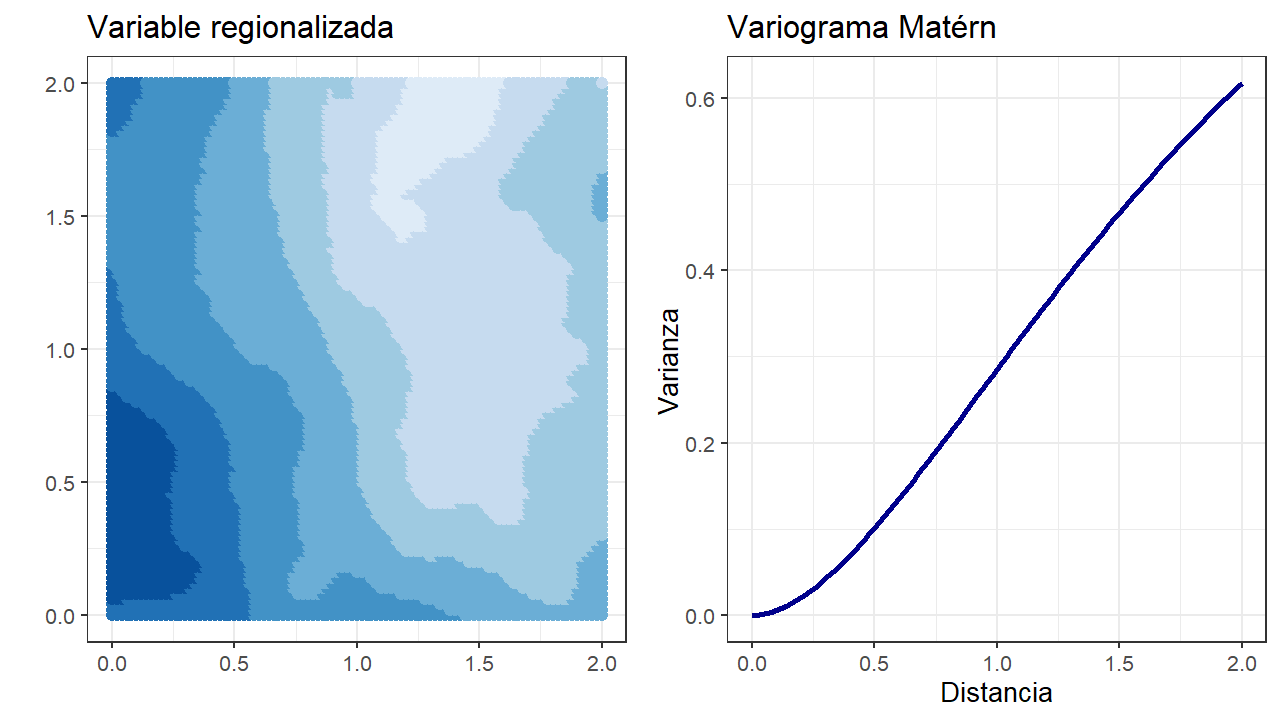
\includegraphics[width=17.78in]{figuras/otros/mat_var} \caption{Izquierda: Variable regionalizada. Derecha: Variograma Matérn.}\label{fig:matvar}
\end{figure}

\hypertarget{variogramas-con-efecto-hueco}{%
\subsubsection*{Variogramas con efecto hueco}\label{variogramas-con-efecto-hueco}}
\addcontentsline{toc}{subsubsection}{Variogramas con efecto hueco}

En la práctica la dependencia espacial puede no crecer monótonamente, incluso esta podría ser negativa o presentar alternaciones entre dependencia espacial positiva y negativa. Estos modelos se llaman \textit{modelos de efecto hueco} y se utilizan para definir oscilaciones que involucran un significado físico. Presentan un comportamiento lineal o parabólico cerca del origen, pueden tener o no tener silla, y pueden ser o no periódicos o pseduperiódicos.

\textbf{Modelo J-Bessel}

Este modelo está definido por:

\begin{align}
    \gamma(||\textbf{h}||;\theta)=\sigma^2\left(1-\left(\frac{2\phi}{||\textbf{h}||} \right)^{\alpha} \Gamma(\alpha+1)J_\alpha \left(\frac{||\textbf{h}||}{\phi} \right) \right),\quad \theta=(\sigma^2,\phi)
\end{align}

donde \(\alpha\) es el parámetro de forma, \(\phi\) es el parámetro de escala, \(\Gamma\) es la función de Euler, y \(J_\alpha\) es la función \(J-Bessel\) del primer tipo de orden \(\alpha\) dada por:

\begin{align}
    J_\alpha (\nu) =\left(\frac{\nu}{2}\right)^2 \sum_{k=0}^\infty{{\frac{-1^k}{k!\Gamma(\alpha+k+1)}}{\left(\frac{\nu}{2}\right)^{2k}}}
\end{align}

y es válido para \(\mathbb{R}^d, d\leq 2(\alpha+1)\).\textbackslash{}

\begin{figure}
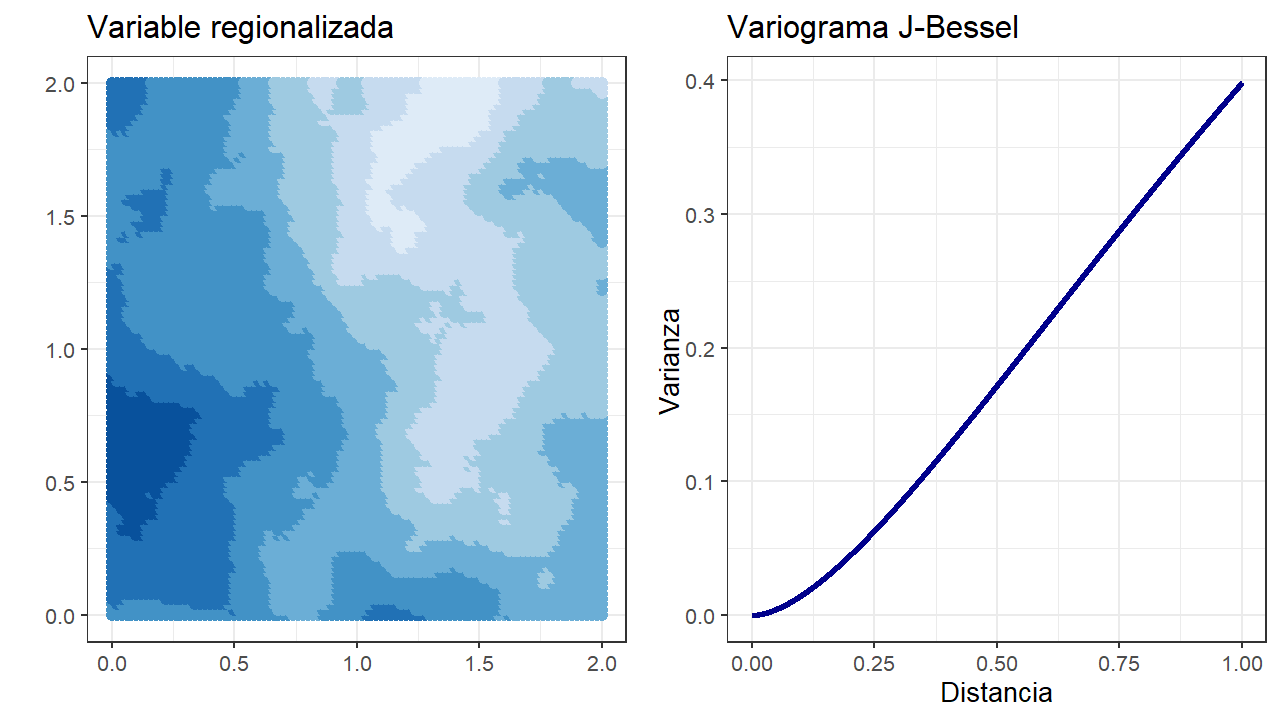
\includegraphics[width=17.78in]{figuras/otros/bes_var} \caption{Izquierda: Variable regionalizada. Derecha: Variograma J-Bessel.}\label{fig:besvar}
\end{figure}

\textbf{Modelo seno cardinal}

Este modelo es una particularización del modelo J-Bessel para \(\alpha=1/2\), y es uno de los pocos modelos de efecto hueco válidos en \(\mathbb{R}^3\), y está definido por:

\begin{align}
    \gamma(||\textbf{h}||;\theta)=\sigma^2 \left(1-\frac{\phi}{||\textbf{h}||}\sin\left(\frac{||\textbf{h}||}{\phi} \right)  \right),\quad \theta=(\sigma^2,\phi)
\end{align}

\begin{figure}
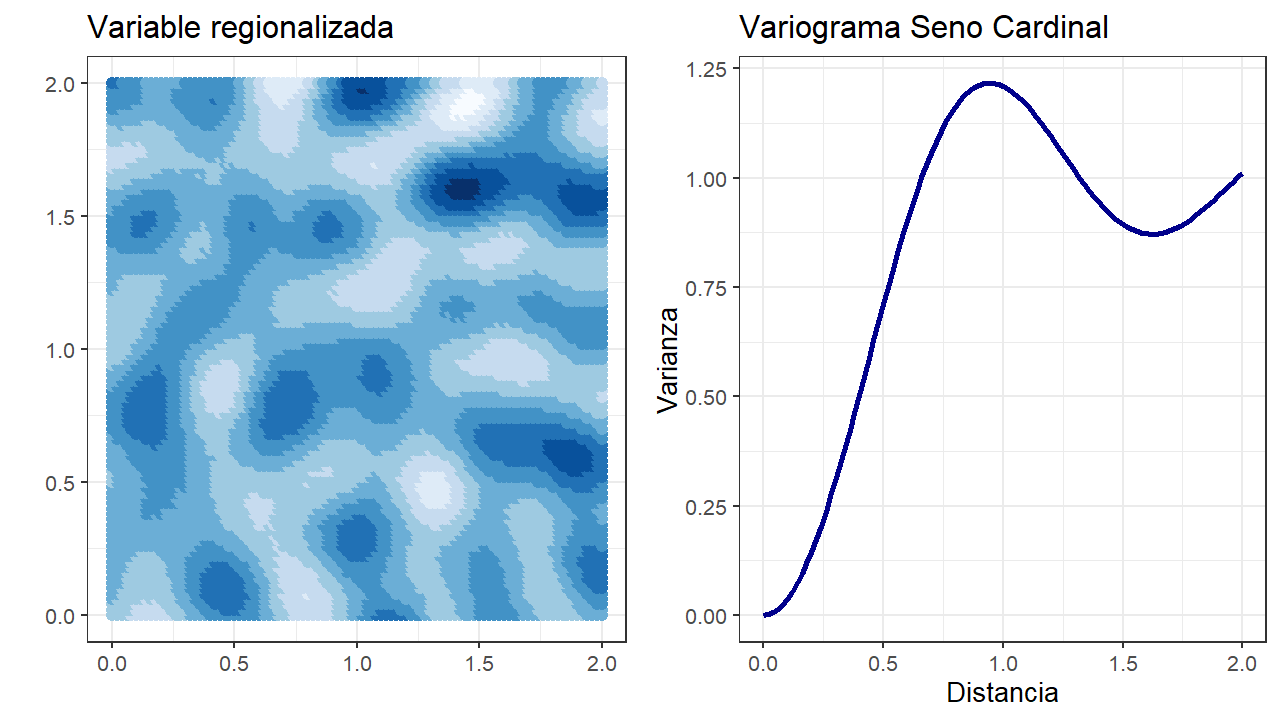
\includegraphics[width=17.78in]{figuras/otros/sin_var} \caption{Izquierda: Variable regionalizada. Derecha: Variograma seno cardinal.}\label{fig:sinvar}
\end{figure}

\hypertarget{variogramas-sin-silla}{%
\subsubsection*{Variogramas sin silla}\label{variogramas-sin-silla}}
\addcontentsline{toc}{subsubsection}{Variogramas sin silla}

Estos modelos corresponden a procesos estocásticos espaciales o campos aleatorios que son intrínsecamente estacionarios, pero no son estacionarios de segundo orden. Estos modelos son no acotados y corresponden a un proceso estocástico espacial o campo aleatorio con capacidad ilimitada para la dispersión espacial y, por consiguiente, ni su covarianza, ni su varianza pueden ser definidas.

\textbf{Modelo Potencia}

Este modelo es válido en \(\mathbb{R}^d,d\geq 1\) y está definido por:

\begin{align}
  \gamma(||\textbf{h}||)=(||\textbf{h}||)^\alpha,\quad  0<\alpha<2, 
\end{align}

Este variograma no posee ni silla ni rango, sino que crece indefinidamente. Si \(\alpha\) es cercano a cero, se dice que es un variograma de efecto pepita, si \(\alpha\) es cercano a dos tiene un comportamiento parabólico y si \(\alpha\) es igual a uno presenta un comportamiento lineal. Para \(\alpha\geq 2\) la condición \(\lim_{h\to \infty}\frac{\gamma||\textbf{h}||}{h^2}=0\) no se satisface; es decir, el modelo no es intrínsecamente estacionario.

\textbf{Modelo lineal}

Este modelo es un caso especial del modelo potencia si \(\alpha=1\), y está asociado con la estacionariedad intrínseca, pero no con la estacionariedad de segundo orden y está definido por:

\begin{align}
  \gamma(||\textbf{h}||)=\left \{ \begin{matrix} 0 & si\ ||\textbf{h}||=0\\
  ||\textbf{h}|| & si\ ||\textbf{h}||>0 \end{matrix}\right.
\end{align}

\hypertarget{caso-multivariante-ejemplos}{%
\subsection{Caso Multivariante (Ejemplos)}\label{caso-multivariante-ejemplos}}

El variograma multivariado fue formalizado en 1991 como una aplicación a procesos estocásticos espaciales o campos aleatorios estacionarios. Para un vector de \(p\) variables regionalizadas estacionarias y para toda métrica \(M\), el covariograma multivariado y el variograma multivariado son definidos como:

\begin{itemize}
\item
  Covariograma multivariado:

  \begin{align}
        K(h)&=E[(Z(s)-\boldsymbol \mu)M(Z(s+\textbf{h})-\boldsymbol \mu){'}]
    \end{align}
\item
  Variograma multivariado:

  \begin{align}
        \Gamma(h)=E[(Z(s)-Z(s+\textbf{h}))M(Z(s)-Z(s+\textbf{h}))']
    \end{align}
\end{itemize}

donde \(Z(s)\) es un vector fila de \(p\) procesos estocásticos espaciales o campos aleatorios estacionarios de segundo orden, \(\boldsymbol \mu=E[Z(s)]\) y \(M\) es una matriz simétrica definida positiva de tamaño \(p\times p\) utilizada como métrica en el cálculo de similaridades (\protect\hyperlink{ref-borou}{\textbf{borou?}}).

Asumiendo estacionariedad de segundo orden, la función de autocovarianza multivariada está relacionada con el variograma multivariado por medio de:

\begin{align}
    K(h)=\Gamma(\infty)-\Gamma(h)
\end{align}

donde \(\Gamma(\infty)\) es la silla del variograma multivariado. Si \(\Gamma(0)=0\) entonces \(K(0)=\Gamma(h)\).

El variograma multivariado representa la esperanza matemática de una medida de disimilitud cuadrática, y la función de autocovarianza multivariada representa la esperanza matemática de una medida de similaridad multivariante (\protect\hyperlink{ref-borou}{\textbf{borou?}}).

La estimación del variograma multivariado se realiza promediando las disimilitudes multivariadas al cuadrado, de forma similar al variograma tradicional; es decir:

\begin{align}
    \Gamma^*(h)=\frac{1}{2|N(\textbf{h})|}\sum_{N(\textbf{h})}d_{ij}^2
\end{align}

donde \(d_{ij}\) es la disimilitud entre las muestras \(i\) y \(j\) calculadas con una métrica dada y \(N(\textbf{h})\) como se definió anteriormente (\protect\hyperlink{ref-borou}{\textbf{borou?}}).

Ahora bien, para realizar el ajuste de los modelos teóricos de variogramas y variogramas cruzados, se utiliza el Modelo Lineal de Coregionalización.

\hypertarget{modelo-lineal-de-coregionalizaciuxf3n-mlc}{%
\subsubsection*{Modelo lineal de coregionalización (MLC)}\label{modelo-lineal-de-coregionalizaciuxf3n-mlc}}
\addcontentsline{toc}{subsubsection}{Modelo lineal de coregionalización (MLC)}

Para el cálculo del MLC es necesario introducir las siguientes medidas:

\begin{itemize}
\item
  \textbf{Covarianza cruzada:}

  \begin{align}
        C_{rr'}(\textbf{h})=\left[E(Z_r(s)-E(Z_r(s))) \right]\left[E(Z_{r'}(s+\textbf{h})-E(Z_{r'}(s+\textbf{h}))) \right]
    \end{align}
\item
  \textbf{Correlación cruzada:}

  \begin{align}
        \rho_{rr'}=\dfrac{C_{rr'}(\textbf{h})}{\sigma_r \sigma_{r'}}
    \end{align}
\item
  \textbf{Variograma cruzado:}

  \begin{align}
        \gamma_{rr'}(\textbf{h})=\frac{1}{2}E\left[Z_r(s+\textbf{h})-Z_r(s) \right]\left[ Z_{r'}(s+\textbf{h})-Z_{r'}(s)\right]
    \end{align}
\item
  \textbf{El pseudo variograma cruzado:}

  \begin{align}
        \phi_{rr'}=\frac{1}{2}E\left[Z_r(s+\textbf{h})-Z_{r'}(s) \right]^2
    \end{align}
\item
  \textbf{Co-dispersión:}

  \begin{align}
        v_{rr'}(\textbf{h})=\frac{\gamma_{rr'}(\textbf{h})}{\sqrt{\gamma_{rr}(\textbf{h})}\sqrt{\gamma_{r'r'}(\textbf{h})} } \in [-1,1]
    \end{align}
\end{itemize}

Al igual que en el caso univariante, el variograma cruzado posee las siguientes propiedades: es invariante bajo traslación, \(\gamma_{rr'}(0)=0\), \(\gamma_{rr'}(\textbf{h})=\gamma_{rr'}(-\textbf{h})\). Además, esta medida es la más utilizada en las aplicaciones geoestadísticas.

Ahora bien, sea \(\mathbb{Z}=(Z_1,...,Z_p)\) un proceso estocástico o campo aleatorio espacial multiavariante; se tiene que el MLC es una suma proporcional de modelos de covarianza o variogramas. En notación matricial donde \(C(\textbf{h})=[C_{ij}(\textbf{h})]\) es una matriz de covarianza de dimensión \(p\times p\) y de manera similar \(\Gamma(\textbf{h})=[\Gamma_{ij}(\textbf{h})]\), con

\begin{align}
    C(\textbf{h})&=\sum_{k=1}^{L}B_kC_k(\textbf{h})\\
    \Gamma(\textbf{h})&=\sum_{k=1}^LB_k\gamma_k(\textbf{h})
\end{align}

donde cada \(B_k\) se conoce como \textit{matriz de coregionalización} y:

\begin{align}
    C_{ij}(\textbf{h})&=\sum_{k=1}^Lb_k(i,j)C_k(\textbf{h})\quad \forall i,j=1,...,p\\
    \Gamma_{ij}(\textbf{h})&=\sum_{k=1}^Lb_k(i,j)\gamma_k(\textbf{h})\quad \forall i,j=1,...,p
\end{align}

El MLC asume que todos los variogramas simples y cruzados pueden ser expresados como una combinación lineal de modelos básicos (exponencial, Gaussiano, esférico, entre otros) idénticos indexados por \(k\). Una condición suficiente para que el modelo sea válido es que cada una de las matrices \(B_k\) sean definidas positivas.

Por construcción del modelo, todos las covarianzas cruzadas son simétricas, y los variogramas cruzados son modelos de variograma válidos.

\hypertarget{ajuste-del-mlc}{%
\subsubsection*{Ajuste del MLC}\label{ajuste-del-mlc}}
\addcontentsline{toc}{subsubsection}{Ajuste del MLC}

El ajuste del MLC puede ser realizado mediante el método de mínimos cuadrados, al igual que en el caso univariante, teniendo en cuenta que la única diferencia es que la silla de cada elemento es reemplazada por una matriz de sillas.

El ajuste es llevado a cabo por el algoritmo propuesto por Goulard (1989) quienes implementaron este algoritmo de manera iterativa para asegurar la positividad de los coeficientes \(B_k\).

Se definen matricialmete el variograma empírico y variograma teórico multivariado como sigue:

\begin{align}
    \hat{\Gamma(\textbf{h})}&=\left[\hat{\gamma}_{ij}(\textbf{h})\right]\\
    \Gamma(\textbf{h})&=\left[\gamma_{ij}(\textbf{h})\right]=\sum_kB_k\gamma_k(\textbf{h})
\end{align}

el criterio de bondad de ajuste es la suma de cuadrados ponderados (SCP) de todos los términos de la matriz de errores \(\hat{\Gamma}(\textbf{h})-\Gamma(\textbf{h})\) y se suman sobre el conjunto de retardos \(J\) utilizados para el ajuste; es decir:

\begin{align}
    SCP=\sum_{k\in J}w(h)\text{traza}\left\{ \left[V^{*}(\hat{\Gamma}(\textbf{h})-\Gamma(\textbf{h}))\right]^2\right\}
\end{align}

Los ponderadores \(w(h)\) son positivos y usualmente iguales al número de pares utilizados para la estimación del variograma en el retardo \(h\). La matriz \(V^{*}\) es definida positiva y diseñada para equilibrar la influencia de las variables; por lo general es la diagonal de la matriz o inversa de la matriz de varianzas o la matriz identidad. La idea es minimizar el criterio optimizando un \(B_k\) a la vez y repitiendo esto hasta que no haya mejora alguna. El residuo para el ajuste actual menos el \(k-\)ésimo término es:

\begin{align}
    d\Gamma_k(\textbf{h})=\hat{\Gamma}(\textbf{h})-\sum_{u\neq k}B_u\gamma_u(\textbf{h})
\end{align}

En ausencia de restricción de positividad, el ajuste óptimo de \(d\Gamma_k\) por \(B_k\gamma_k(\textbf{h})\) se obtiene por medio de la cancelación de la derivada de SCP en relación a \(B_k\)

\begin{align}
    \frac{\partial SCP}{\partial B_k}=-2V^{*}\left[ \sum_{h\in J}w(h)\gamma_k(\textbf{h})\left(d\Gamma_k(\textbf{h})-\gamma_k(\textbf{h})B_k\right)\right]V^{*}=0
\end{align}

Como \(V^{*}\) es no singular se tiene que:

\begin{align}
    B_k&=\frac{1}{\alpha_k}\sum_{h\in J}w(h)\gamma_k(\textbf{h})d\Gamma_k(\textbf{h})\\
\end{align}

donde

\begin{align}
    \alpha_k&=\sum_{h\in J}w(h)\gamma_k(\textbf{h})^2
\end{align}

La solución restringida \(B_k^{+} \geq 0\) es la matriz definida positiva cercana a \(B_k\) de acuerdo a la norma definida por \(V^{*}\). Dado que es simétrica, la matriz \(B_k\) tiene descomposición de la siguiente forma

\begin{align}
    B_k=U_k\nabla_k U_k^{'}\quad \text{con} \quad U_k^{'}V^{*}U_k=I_p
\end{align}

donde \(U_k\) es una matriz de vectores propios de \(B_kV^{*}\) y \(\nabla_k\) es la matriz diagonal de sus valores propios.

Por tanto, la solución restringida es

\begin{align}
    B_k^{'}=U_k\nabla_k^{+}U_k^{'}
\end{align}

donde \(\nabla_k^{+}\) es la matriz \(\nabla_k\) en el cual los valores propios negativos son reemplazados por ceros. Este algoritmo iterativo siempre converge y la solución no depende del punto de partida (\protect\hyperlink{ref-peter}{\textbf{peter?}}).

\hypertarget{geoestaduxedstica-espacio-temporal}{%
\section{Geoestadística Espacio Temporal}\label{geoestaduxedstica-espacio-temporal}}

A través de la geoestadística se han estudiado los campos aleatorios en la naturaleza; sin embargo, existen ramas de la ciencia que presentan aplicaciones prácticas como las ciencias sociales, monitorización de contaminación ambiental, climatología, geología, biología, medicina, arqueología y cualquier otro campo de la ciencia que estudie fenómenos que ocurren tanto en espacio como en tiempo (\protect\hyperlink{ref-montero}{\textbf{montero?}}). Al considerar la evolución conjunta del proceso espacio-temporal, en lugar de solo considerar su distribución espacial para un determinado instante de tiempo (proceso puramente espacial) o la evolución temporal del proceso sobre una localización determinada (proceso puramente temporal), se obtendrá grandes beneficios en la modelización y predicción de un fenómeno en estudio (\protect\hyperlink{ref-gstcasal}{\textbf{gstcasal?}}). Es así que considerar ambos elementos por separado nos llevaría a una pérdida de información. En este sentido, la geoestadística espacio-temporal ofrece las herramientas adecuadas para este tipo de estudios.Es por ello que la demanda de modelos covariográficos que describen la evolución de procesos en espacio-tiempo se hace cada vez más notoria.

Los métodos geoestadísticos y espacio-temporales utilizan distancias euclídeas o espacio temporales, por tanto se consideran los métdos basados en distancias para el cálculo entre las observaciones que junto la información proporcionada por el variograma permitirá la generación de mejores pronósticos (\protect\hyperlink{ref-gstcasal}{\textbf{gstcasal?}}). Por otro lado se debe considerar que en el campo espacio-tiempo también se trabaja con grandes volúmenes de datos debido a la resolución espacial y periodicidad temporal, lo que conlleva al uso de métodos computacionales intensivos.

\hypertarget{conceptos}{%
\subsection{Conceptos}\label{conceptos}}

Se puede considerar a cada ubicación espacio-temporal como un punto en \(\mathbb{R}^d \times \mathbb{R}\), con \(\mathbb{R}^d\) siendo el espacio euclidiano \(d-\)dimensional y \(\mathbb{R}\) la dimensión del tiempo. Notemos que ni las escalas ni las unidades de distancia en el tiempo y el espacio son generalmente comparables. Por lo que la dificultad principal en el análisis de procesos espacio-temporales recae en la elección de un modelo de covarianza válido que se ajuste a las observaciones. Bajo hipótesis de regularidad se podrán analizar las observaciones separadas por un vector de distancia espacio temporal \((\textbf{h},u)\) (\protect\hyperlink{ref-gstcasal}{\textbf{gstcasal?}}).

El objetivo de esta sección es introducir aquellos conceptos más relevantes en el análisis de procesos estocásticos espacio-temporales. Muchos de los conceptos tratados serán generalizaciones del caso espacial que se han visto en el capítulo \textbf{X}.

\hypertarget{proceso-espacio-temporal-1}{%
\subsubsection*{Proceso Espacio Temporal}\label{proceso-espacio-temporal-1}}
\addcontentsline{toc}{subsubsection}{Proceso Espacio Temporal}

Sea \(Z\) la variable aleatoria de interés, \(s\) su ubicación espacial y \(t\) el tiempo de ocurrencia. Un proceso espacio-temporal es un proceso estocástico

\begin{align}
  \{Z(s,t):(s,t) \in D \times D' \}
\end{align}

donde el conjunto \(D \subset \mathbb{R}^d\) es el conjunto de todas las ubicaciones espaciales y el conjunto \(D' \subset \mathbb{R}\) es el conjunto de todos los instantes de tiempo. Los conjuntos \(D\) y \(D'\) pueden ser continuos o discretos, fijos o aleatorios (\protect\hyperlink{ref-marta}{\textbf{marta?}}).

Siguiendo los conceptos clásicos de geoestadística, la distribución del proceso espacio-temporal es modelado como una distribucín Gaussiana. Esta distribución será caracterizada definiendo su momento de primer orden y su momento de segundo orden, es decir, su esperanza y función de covarianza (\protect\hyperlink{ref-montero}{\textbf{montero?}}).

\hypertarget{propiedad-de-regularidad}{%
\subsubsection*{Propiedad de regularidad}\label{propiedad-de-regularidad}}
\addcontentsline{toc}{subsubsection}{Propiedad de regularidad}

Un campo aleatorio \(Z(s,t)\) en \(\mathbb{R}^d\times \mathbb{R}\) cumple la propiedad de regularidad si:

\begin{align}
V(Z(s,t))<\infty, \forall (s,t) \in \mathbb{R}^d\times \mathbb{R}
\end{align}

que a su vez asegura la existencia de los dos primeros momentos.

\hypertarget{campo-aleatorio-gaussiano}{%
\subsubsection*{Campo aleatorio Gaussiano}\label{campo-aleatorio-gaussiano}}
\addcontentsline{toc}{subsubsection}{Campo aleatorio Gaussiano}

Un campo aleatorio \(Z(s,t)\) se dice Gaussiano si el vector aleatorio \(\textbf{Z}=(Z(s_1,t_1),...,Z(s_n,t_n))\) para cualquier conjunto de ubicaciones espacio-temporales \({(s_1,t_1),...,(s_n,t_n)}\), sigue una distribución Gaussiana multivariante.

\hypertarget{funciuxf3n-de-media-1}{%
\subsubsection*{Función de media}\label{funciuxf3n-de-media-1}}
\addcontentsline{toc}{subsubsection}{Función de media}

La media de un campo aleatorio espacio-temporal está definido por la función

\begin{align}
  E[Z(s,t)]=\mu(s,t)
  \end{align}

\hypertarget{funciuxf3n-de-covarianza-1}{%
\subsubsection*{Función de covarianza}\label{funciuxf3n-de-covarianza-1}}
\addcontentsline{toc}{subsubsection}{Función de covarianza}

Para cualquier para de puntos espacio-temporales, la covarianza de un campo aleatorio espacio temporal está definido por la función

\begin{align}
C[(s_i,t_i),(s_j,t_j)]=C[Z(s_i,t_i),Z(s_j,t_j)]
\end{align}

\hypertarget{estacionariedad-fuerte-o-estricta}{%
\subsubsection*{Estacionariedad fuerte o estricta}\label{estacionariedad-fuerte-o-estricta}}
\addcontentsline{toc}{subsubsection}{Estacionariedad fuerte o estricta}

Un campo aleatorio \(Z(s,t)\) es estrictamente estacionario si su distribución de probabilidad es traslacionalmente invariante. Es decir que, para dos vectores \(\textbf{h}\) y \(u\)

\begin{align}
Z(s,t)&=[Z(s_1,t_1), Z(s_2,t_2),...,Z(s_n,t_n)]^{'}
\end{align}

y

\begin{align}
Z(s+\textbf{h},t+u)&=[Z(s_1+\textbf{h},t_1+u), Z(s_2+\textbf{h},t_2+u),...,Z(s_n+\textbf{h},t_n+u)]^{'}
\end{align}

Tienen la misma función de distribución multivariante, es decir

\begin{align}
F_{Z_1,...,Z_n}[(s_1,t_1),...,(s_n,t_n)]&= F_{Z_1,...,Z_n}[(s_1+\textbf{h},t_1+ u),...,(s_n+\textbf{h},t_n+u)]
\end{align}

\hypertarget{estacionariedad-de-segundo-orden-1}{%
\subsubsection*{Estacionariedad de segundo orden}\label{estacionariedad-de-segundo-orden-1}}
\addcontentsline{toc}{subsubsection}{Estacionariedad de segundo orden}

Un campo aleatorio \(Z(s,t)\) es estacionario de segundo orden si tiene media constante y la función de covarianza depende solo de \(\textbf{h}\) y \(u\), es decir

\begin{align}
E[Z(s,t)]&=\mu(s,t)=\mu,\quad \forall (s,t)\in \mathbb{R}^2\times \mathbb{R} \\
C[Z(s_i,t_i),Z(s_j,t_j)]&=C(\textbf{h}, u), \quad \forall(s,t) \in \mathbb{R}^2 \times \mathbb{R}
\end{align}

\hypertarget{estacionariedad-intruxednseca-1}{%
\subsubsection*{Estacionariedad intrínseca}\label{estacionariedad-intruxednseca-1}}
\addcontentsline{toc}{subsubsection}{Estacionariedad intrínseca}

Un campo aleatorio espacio-temporal \(Z(s,t)\) es intrínsecamente estacionario si el proceso de incrementos \(Z(s+\textbf{h},t+u)-Z(s,t)\) es estacionario de segundo orden en espacio-tiempo para cualquier \((\textbf{h},t)\) fijo.

\hypertarget{funciuxf3n-de-covarianza-estacionaria-espacial}{%
\subsubsection*{Función de covarianza estacionaria espacial}\label{funciuxf3n-de-covarianza-estacionaria-espacial}}
\addcontentsline{toc}{subsubsection}{Función de covarianza estacionaria espacial}

Un campo aleatorio espacio-temporal \(Z(s,t)\) tiene función de covarianza estacionaria espacial si, para cualquier par de puntos \((s_i,t_i),\ (s_j,t_j) \in \mathbb{R}^d \times \mathbb{R}\) la función de covarianza \(C[(s_i,t_i),(s_j,t_j)]\) solo depende de la distancia entre las ubicaciones \((s_i-s_j)\) y los tiempos \(t_i,\ t_j\).

\hypertarget{funciuxf3n-de-covarianza-estacionaria-temporal}{%
\subsubsection*{Función de covarianza estacionaria temporal}\label{funciuxf3n-de-covarianza-estacionaria-temporal}}
\addcontentsline{toc}{subsubsection}{Función de covarianza estacionaria temporal}

Un campo aleatorio espacio-temporal \(Z(s,t)\) tiene función de covarianza estacionaria espacial si, para cualquier par de puntos \((s_i,t_i),\ (s_j,t_j) \in \mathbb{R}^d \times \mathbb{R}\) la función de covarianza \(C[(s_i,t_i),(s_j,t_j)]\) solo depende de la distancia entre los tiempos \((t_i-t_j)\) y de las ubicaciones espaciales \(s_i,\ s_j\).

\hypertarget{funciuxf3n-de-covarianza-estacionaria-espacio-temporal}{%
\subsubsection*{Función de covarianza estacionaria espacio-temporal}\label{funciuxf3n-de-covarianza-estacionaria-espacio-temporal}}
\addcontentsline{toc}{subsubsection}{Función de covarianza estacionaria espacio-temporal}

Si el campo aleatorio \(Z(s,t)\) tiene función de covarianza en términos de espacio y de tiempo, entonces se dice que tiene función de covarianza estacionaria y puede ser expresada de la siguiente forma

\begin{align}
C[(s_i,t_i),(s_j,t_j)]=C[\textbf{h},u]
\end{align}

donde \(\textbf{h}=s_i-s_j\) y \(u=t_i-t_j\) son las distancias en espacio y en tiempo respectivamente.

Si un proceso espacio-temporal tiene función de covarianza estacionaria, entonces su varianza no depende de la ubicación espaio-temporal, pues

\begin{align}
Var(Z(s,t))=C(\boldsymbol 0,0)=\sigma^2,\ \forall (s,t) \in \mathbb{R}^d \times \mathbb{R}
\end{align}

donde \(C(\boldsymbol 0,0) \geq 0\) se conoce como la varianza a priori del proceso.

\hypertarget{funciuxf3n-de-covarianza-separable}{%
\subsubsection*{Función de covarianza separable}\label{funciuxf3n-de-covarianza-separable}}
\addcontentsline{toc}{subsubsection}{Función de covarianza separable}

Un campo aleatorio \(Z(s,t)\) tiene función de covarianza separable si tiene función de covarianza puramente espacial \(C_s(s_i,s_j)\) y función de covarianza puramente temporal \(C_t(t_i,t_j)\) tal que

\begin{align}
C[(s_i,t_i),(s_j,t_j)]&=C_s(s_i,s_j)C_t(t_i,t_j) 
\label{eq:separ}
\end{align}

para cualquier par de puntos espacio-temporales \((s_i,t_i),\ (s_j,t_j)\in \mathbb{R}^d\times \mathbb{R}\). Si esta descomposición no es posible , la función de covarianza se llamará \textbf{no separable}.

Al descomponer la covarianza de acuerdo con \eqref{eq:separ} permite mayor eficiencia en términos computacionales. Es por esto que los modelos separables han sido ampliamente utilizados en aplicaciones geoestadísticas, inclusive en situaciones donde esta hipótesis no se justifica por la naturaleza del proceso bajo análisis.

\hypertarget{funciuxf3n-de-covarianza-simuxe9trica}{%
\subsubsection*{Función de covarianza simétrica}\label{funciuxf3n-de-covarianza-simuxe9trica}}
\addcontentsline{toc}{subsubsection}{Función de covarianza simétrica}

Un campo aleatorio espacio-temporal \(Z(s,t)\) tiene función de covarianza simétrica si para cualquier par de puntos espacio-temporales \((s_i,t_i),\ (s_j,t_j)\in \mathbb{R}^d \times \mathbb{R}\) se tiene que

\begin{align}
  C[(s_i,t_i),(s_j,t_j)]=C[(s_i,t_j),(s_j,t_i)]
\end{align}

Nótese que la separabilidad es un caso particular de la propiedad de simetría.

En el caso de tener función de covarianza espacio-temporal estacionaria, \(\forall (\textbf{h},u)\in \mathbb{R}^d \times \mathbb{R}\) la propiedad de simetría se puede representar de la siguiente manera

\begin{align}
C(\textbf{h}, u)&=C(\textbf{h},-u)\\
&=C(-\textbf{h}, u)\\
&=C(-\textbf{h}, -u)
\end{align}

\hypertarget{funciuxf3n-de-covarianza-espacialmente-isotruxf3pica}{%
\subsubsection*{Función de covarianza espacialmente isotrópica}\label{funciuxf3n-de-covarianza-espacialmente-isotruxf3pica}}
\addcontentsline{toc}{subsubsection}{Función de covarianza espacialmente isotrópica}

Un campo aleatorio espacio-temporal \(Z(s,t)\) tiene función de covarianza espacialmente isotrópica si

\begin{align}
C(\textbf{h},u)=C(||\textbf{h}||,u), \ \forall(s,t) \in \mathbb{R}^d \times \mathbb{R}
\end{align}

\hypertarget{funciuxf3n-de-covarianza-temporalmente-isotruxf3pica}{%
\subsubsection*{Función de covarianza temporalmente isotrópica}\label{funciuxf3n-de-covarianza-temporalmente-isotruxf3pica}}
\addcontentsline{toc}{subsubsection}{Función de covarianza temporalmente isotrópica}

Un campo aleatorio espacio-temporal \(Z(s,t)\) tiene función de covarianza temporalmente isotrópica si

\begin{align}
C(\textbf{h},u)=C(\textbf{h},|u|), \ \forall(s,t) \in \mathbb{R}^d \times \mathbb{R}
\end{align}

Nótese que si la función de covarianza de un campo aleatorio espacio-temporal es estacionaria con respecto a espacio y tiempo, entonces es simétrica (\protect\hyperlink{ref-montero}{\textbf{montero?}}).

Al igual que en el caso de la geoestadística clásica, es frecuente el uso del variograma para la modelización de la estructura espacio-temporal de un campo aleatorio.

\hypertarget{variograma-espacio-temporal}{%
\subsubsection*{Variograma espacio-temporal}\label{variograma-espacio-temporal}}
\addcontentsline{toc}{subsubsection}{Variograma espacio-temporal}

La función de variograma espacio-temporal está definido de la siguiente forma

\begin{align}
\gamma[(s_i,t_i),(s_j,t_j)]&=\frac{1}{2}V[Z(s_i,t_i)-Z(s_j,t_j)]
\end{align}

En el caso de un campo aleatorio con media constante se tiene que

\begin{align}
\gamma[(s_i,t_i),(s_j,t_j)]&=\frac{1}{2}E[Z(s_i,t_i)-Z(s_j,t_j)]^2
\end{align}

Siempre que sea posible definir la función de covarianza y la función de variograma, estas estarán relacionadas de acuerdo a lo siguiente

\begin{align}
\gamma[(s_i,t_i),(s_j,t_j)]&=\frac{1}{2}V[Z(s_i,t_i)]+\frac{1}{2}V[Z(s_j,t_j)]-C[(s_i,t_i),(s_j,t_j)]
\label{eq:varivar}
\end{align}

\hypertarget{variograma-espacio-temporal-intruxednsecamente-estacionario-espacial}{%
\subsubsection*{Variograma espacio-temporal intrínsecamente estacionario espacial}\label{variograma-espacio-temporal-intruxednsecamente-estacionario-espacial}}
\addcontentsline{toc}{subsubsection}{Variograma espacio-temporal intrínsecamente estacionario espacial}

Un campo aleatorio \(Z(s,t)\) tiene variograma intrínsecamente estacionario con respecto al espacio si, para cualquier para de puntos espacio-temporales \((s_i,t_i), \ (s_j,t_j) \in \mathbb{R}^d \times \mathbb{R}\), el variograma \(\gamma[(s_i,t_i),(s_j,t_j)]\) solo depende de \(\textbf{h}=s_i-s_j\) y los tiempos \(t_i\) y \(t_j\).

\hypertarget{variograma-espacio-temporal-intruxednsecamente-estacionario-temporal}{%
\subsubsection*{Variograma espacio-temporal intrínsecamente estacionario temporal}\label{variograma-espacio-temporal-intruxednsecamente-estacionario-temporal}}
\addcontentsline{toc}{subsubsection}{Variograma espacio-temporal intrínsecamente estacionario temporal}

Un campo aleatorio \(Z(s,t)\) tiene variograma intrínsecamente estacionario con respecto al tiempo si, para cualquier para de puntos espacio-temporales \((s_i,t_i), \ (s_j,t_j) \in \mathbb{R}^d \times \mathbb{R}\), el variograma \(\gamma[(s_i,t_i),(s_j,t_j)]\) solo depende de \(u=t_i-t_j\) y las ubicaciones \(s_i\) y \(s_j\).

\hypertarget{variograma-espacio-temporal-intruxednsecamente-estacionario}{%
\subsubsection*{Variograma espacio-temporal intrínsecamente estacionario}\label{variograma-espacio-temporal-intruxednsecamente-estacionario}}
\addcontentsline{toc}{subsubsection}{Variograma espacio-temporal intrínsecamente estacionario}

Un campo aleatorio \(Z(s,t)\) tiene variograma intrínsecamente estacionario si, su variograma es intrínsecamente estacionario en espacio y tiempo. En este caso, el variograma se puede expresar de la siguiente forma

\begin{align}
\gamma[(s_i,t_i),(s_j,t_j)]=\gamma(\textbf{h},u)
\end{align}

donde \(\textbf{h}=s_i-s_j\) y \(u=t_i-t_j\) representan la distancia en espacio y tiempo respectivamente.

Dado un campo aleatorio estacionario de segundo orden \(Z(s,t)\) con función de covarianza \(C(\textbf{h},u)\), debido a \eqref{eq:varivar}, se cumple que

\begin{align}
V[Z(s_i,t_i)-Z(s_j,t_j)]&=V[Z(s_i,t_i)]+V[Z(s_j,t_j)]-2C[(s_i,t_i),(s_j,t_j)]\\
&=2C(\textbf{0},0)-2C(s_i-s_j,t_i-t_j)
\end{align}

por tanto el campo aleatorio \(Z(s,t)\) será intrínsecamente estacionario con variograma

\begin{align}
\gamma(\textbf{h},u)=C(\textbf{0},0)-C(\textbf{h},u)
\end{align}

\hypertarget{funciuxf3n-de-correlaciuxf3n-espacio-temporal}{%
\subsubsection*{Función de correlación espacio-temporal}\label{funciuxf3n-de-correlaciuxf3n-espacio-temporal}}
\addcontentsline{toc}{subsubsection}{Función de correlación espacio-temporal}

Sea \(Z(s,t)\) un campo aleatorio espacio-temporal estacionario de segundo orden con varianza a priori \(\sigma^2 = C(\textbf{0},0)>0\). La función de correlación se define como sigue

\begin{align}
\rho(\textbf{h},u)=\frac{C(\textbf{h},u)}{C(\textbf{0},u)}
\end{align}

si \(\rho(\textbf{h},u)\) es función de correlación en \(\mathbb{R}^d \times \mathbb{R}\), entonces sus funciones marginales \(\rho(\textbf{0},u)\) y \(\rho(\textbf{h},0)\) serán funciones de correlación espacial en \(\mathbb{R}^d\) y temporal en \(\mathbb{R}\) respectivamente.

\hypertarget{propiedades-de-la-covarianza-y-variograma-espacio-temporal}{%
\subsubsection{Propiedades de la covarianza y variograma espacio-temporal}\label{propiedades-de-la-covarianza-y-variograma-espacio-temporal}}

Una condición necesaria y suficiente para que la función de valores reales \(C[(s_i,t_i),(s_j,t_j)]\) definido en \(\mathbb{R}^d \times \mathbb{R}\) sea una función de covarianza es que sea simétrica y definida positiva, es decir

\begin{align}
C[(s_i,t_i),(s_j,t_j)]&=C[(s_j,t_j),(s_i,t_i)]\\
\sum_
{i=1}^{n}\sum_
{j=1}^{n}a_ia_j&C[(s_i,t_i),(s_j,t_j)] \geq 0
\end{align}

para cualquier \(n\in \mathbb{N}\) y para cualquier \((s_i,t_i) \in \mathbb{R}^d \times \mathbb{R}\) y \(a_i\in \mathbb{R},\ i=1,...,n\).

De manera similar, una condición necesaria y suficiente para una función no negativa de valores reales \(\gamma[(s_i,t_i),(s_j,t_j)]\) definidas en \(\mathbb{R}^d \times \mathbb{R}\) para que una función de variograma es que sea simétrica y condiconalmente definida negativa, es decir

\begin{align}
\gamma[(s_i,t_i),(s_j,t_j)]&=\gamma[(s_j,t_j),(s_i,t_i)]\\
\sum_
{i=1}^{n}\sum_
{j=1}^{n}a_ia_j&\gamma[(s_i,t_i),(s_j,t_j)] \leq 0
\end{align}

para cualquier \(n\in \mathbb{N}\) y para cualquier \((s_i,t_i) \in \mathbb{R}^d \times \mathbb{R}\) y \(a_i\in \mathbb{R},\ i=1,...,n\) con \(\sum_{i=1}^na_i=0\).

En el caso de estacionariedad, se puede deducir que la fucnipon de valores reales \(C(\textbf{h},u)\) definido en \(\mathbb{R}^d \times \mathbb{R}\) es una función de covarianza, si y solo si, es una función par y definida positiva, es decir

\begin{align}
C(\textbf{h},u)&=C(-\textbf{h},-u)\\
\sum_
{i=1}^{n}\sum_
{j=1}^{n}a_i&a_jC(\textbf{h}_i,u_i) \geq 0
\end{align}

para cualquier \(n\in \mathbb{R}\) y para cualquier \((\textbf{h}_i,u_i) \in \mathbb{R}^d \times \mathbb{R},\ a_i \in \mathbb{R}, \ i=1,...,n\).

En este sentido, una función no negativa de valores reales \(\gamma(\textbf{h},u)\) definida en \(\mathbb{R}^d \times \mathbb{R}\) es una función de variograma intrínsecamente estacionaria, si y solo si, es una función para y condicionalmente definida negativa, es decir

\begin{align}
\gamma(\textbf{h},u)&=\gamma(-\textbf{h},-u)\\
\sum_
{i=1}^{n}\sum_
{j=1}^{n}a_i&a_j\gamma(\textbf{h}_i,u_i) \leq 0
\end{align}

para cualquier \(n\in \mathbb{R}\) y para cualquier \((\textbf{h}_i,u_i) \in \mathbb{R}^d \times \mathbb{R},\ a_i \in \mathbb{R}, \ i=1,...,n\) con \(\sum_{i=1}^na_i=0\)

Algunas de las propiedades más importantes son las siguientes

\begin{itemize}
\tightlist
\item
  Si \(C_1(\text{h},u)\) es una función de covariazna definida en \(\mathbb{R}^d \times \mathbb{R}\) y \(b>0\), entonces
\end{itemize}

\begin{align}
C(\text{h},u)=bC_1(\text{h},u)
\end{align}

\begin{itemize}
\tightlist
\item
  Sean \(C_1(\textbf{h},u)\) y \(C_2(\textbf{h},u)\) dos fucniones de covariana definidas en \(\mathbb{R}^d \times \mathbb{R}\), entonces
\end{itemize}

\begin{align}
C(\textbf{h},u)&=C_1(\textbf{h},u)+C_2(\textbf{h},u)
\end{align}

es también una función de covarianza definida en \(\mathbb{R}^d \times \mathbb{R}\).

\begin{itemize}
\tightlist
\item
  Dadas dos funciones de covarianza \(C_1(\textbf{h},u)\) y \(C_2(\textbf{h},u)\) definidas en \(\mathbb{R}^d \times \mathbb{R}\), entonces
\end{itemize}

\begin{align}
C(\textbf{h},u)&=C_1(\textbf{h},u)C_2(\textbf{h},u)
\end{align}

es también una función de covarianza definida en \(\mathbb{R}^d\times \mathbb{R}\).

\begin{itemize}
\tightlist
\item
  Si \(\{C_n(\textbf{h},u),n=1,...,\}\) es una secuencia de funciones de covaraizna definidas en \(\mathbb{R}^d \times \mathbb{R}\) convergen a \(C(\textbf{h},u), \forall (\textbf{h},u) \in \mathbb{R}^d \times \mathbb{R}\), entonces
\end{itemize}

\begin{align}
C(\textbf{h},u)&=\lim_{n\to 2} C_n(\textbf{h},u)
\end{align}

es una función de covarianza en \(\mathbb{R}^d \times \mathbb{R}\).

\hypertarget{estimaciuxf3n-del-variograma-y-covariograma-espacio-temporal}{%
\subsection{Estimación del variograma y covariograma espacio-temporal}\label{estimaciuxf3n-del-variograma-y-covariograma-espacio-temporal}}

La estimación del variograma o covariograma espacio-temporal puede ser la generalización de la estimación de un proceso espacial. Es así que, sea \(Z(s,t)\) un proceso intrinsecamente estacionario sobre un conjunto de \(n\) ubicaciones espacio-temporales \(\{(s_1,t_1),...,(s_n.t_n)\}\).
Usualmente se utilizan dos alternativas para estimar el variograma \(\gamma(.,.)\) o covariograma \({\hat{C}(.,.)}\), utilizando los valores observados:

\hypertarget{estimadores-cluxe1sicos}{%
\subsubsection{Estimadores clásicos}\label{estimadores-cluxe1sicos}}

\textbf{Estimador empírico del variograma}

El estimador empírico del variograma, propuesto por Matheron, está basado en el método de momentos y está dado por:

\begin{align}
{\hat{\gamma}}(\textbf{h}(l),u(k))=\frac{1}{2|N(\textbf{h}(l),u(k))|} \sum_{(s_i,t_i),(s_j,t_j)\in N(\textbf{h}(l),u(k))} [Z(s_i,t_i)-Z(s_j,t_j)]^2
\end{align}

donde \(N(\textbf{h}(l),u(k))=\{(s_i,t_i)(s_j,t_j):s_i -s_j \in T(\textbf{h}(l)), t_i-t_j \in T(u(k))\}\), \(T(\textbf{h}(l))\)es la region de tolerancia sobre \(\mathbb{R}^d\) alrededor de \(\textbf{h}(l)\) y \(T(u(k))\) es una región de tolerancia sobre \(\mathbb{R}\) alrededor de \(u(k)\) y \(|N(\textbf{h}(l),u(k))|\) es el número de elementos diferentes en \(N(\textbf{h}(l),u(k))\) con \(l=1,...,L\) y \(k=1,...,K\)

Si se asume isotropía para el proceso espacial, se puede elegir \(T(\textbf{h}(l))\) alrededor de cada valor \(\textbf{h}(l)\) como \(\left[h(l)-\frac{d_1}{2}, h(l)+\frac{d_1}{2}\right]\) donde \(d_1\) es la tolerancia espacial utilizada.También es común elegir valores en \(\mathbb{Z}\) para el componente temporal, en este caso el variograma empirico es calculado para \(u(k)=0,1,,...\) que se obtiene como las sucesivas diferencias de tiempo en que se observa el proceso.

\textbf{Estimador empírico del covariograma}

El estimador empírico de la función de covariograma utilizando el método de momentos está dado por

\begin{align}
{\hat{C}}(\textbf{h}(l),u(k))=\frac{1}{|N(\textbf{h}(l),u(k))|} \sum_{(s_i,t_i),(s_j,t_j)\in N(\textbf{h}(l),u(k))} [Z(s_i,t_i)-{\bar{Z}}][Z(s_j,t_j)-\bar{Z}]
\end{align}

donde \(\bar{Z}=\frac{1}{n} \sum_{i} Z(s_i , t_i)\) es un estimador de la media \(\mu\) de un campo aleatorio y \(N(\textbf{h}(l),u(k))\) al igual que en los casos anteriores.

Al igual que en el caso de geoestadística clásica los estimadores presentados anteriormente son susceptibles a valores atípicos o extremos para evitar este problema se considera el siguiente estimador robusto.

\hypertarget{estimador-robusto-por-cressie-y-hawkins}{%
\subsubsection{Estimador robusto por Cressie y Hawkins}\label{estimador-robusto-por-cressie-y-hawkins}}

Este estimador espacio-temporal de la función de variograma se define de por

\begin{align}
{\hat{\gamma}}(\textbf{h}(l),u(k))&=\left({\frac{1}{2|N(\textbf{h}(l),u(k))|}}{\sum_{(s_i,t_i),(s_j,t_j)\in N(\textbf{h}(l),u(k))} {|Z(s_i,t_i)-Z(s_j,t_j)|^{\frac{1}{2}}}}\right)^4\\
& \times \left(0.457 + \frac{0.494}{|N(\textbf{h}(l),u(k))|} \right)^{-1}
\end{align}

ejercicio para el lector: calcular el covariograma

\hypertarget{introducciuxf3n-al-anuxe1lisis-de-datos-funcionales-fda}{%
\chapter{Introducción al análisis de datos funcionales (FDA)}\label{introducciuxf3n-al-anuxe1lisis-de-datos-funcionales-fda}}

Los objetivos fundamentales del FDA son los mismos que la estadística convencional e incluyen: (a) Representar y transformar los datos de manera que faciliten el análisis posterior. (b) Mostrar los datos de manera que se destaquen las variables en estudio. (c) Estudiar fuentes relevantes de patrones y variación de los datos. (d) Explicar la variación de una variable resultante o dependiente utilizando la información de la variable independiente (\protect\hyperlink{ref-raichle}{\textbf{raichle?}}).

En la estadística elemental las observaciones son escalares, pero en la estadística multivariante las observaciones son vectores que pertenecen al espacio Euclídeo \(\mathbb{R}^d\), donde \(d\) es la dimensión de los vectores observados. Sin embargo, en el FDA las observaciones son funciones o curvas y aunque estas pueden ser medidas en puntos discretos se las pueden pensar como funciones en espacios infinitos dimensionales (\protect\hyperlink{ref-kokoska}{\textbf{kokoska?}}).

Los datos funcionales por tanto son una generalización natural de datos multivariantes, pasando de una dimensión finita a una dimensión infinita (\protect\hyperlink{ref-jin}{\textbf{jin?}}). La alta dimensionalidad de los datos, representa un reto para la teoría y para el cálculo computacional, donde estos retos varían dependiendo de como se tomaron las muestras. Sin embargo, la alta o infinita dimensionalidad de los datos, son una fuente rica en información, lo que conlleva a poder realizar investigaciones y análisis de datos mas robustos (\protect\hyperlink{ref-wang}{\textbf{wang?}}).

La extensa variedad de aplicaciones y herramientas hacen que definir de forma precisa el FDA sea de cierta manera difícil. El FDA surge cuando una variable de interés, en un conjunto de datos, puede ser naturalmente vista como una curva o función suave; entonces el FDA puede pensarse como un análisis de alto nivel estadístico sobre muestras de curvas (\protect\hyperlink{ref-kokoska}{\textbf{kokoska?}}). En la práctica, los datos funcionales son obtenidos por medio de observaciones sobre el tiempo, {ESPACIO} u otros dominios continuos; los datos funcionales resultantes pueden ser curvas, superficies u objetos complejos (\protect\hyperlink{ref-jin}{\textbf{jin?}}).

{iNSERTAR IMÁGENES DATO FUNCIONAL CON DOMINIOS}

Las funciones o curvas pueden ser vistas como realizaciones de un proceso estocástico uno dimensional; usualmente se asume que estas realizaciones pertenecen al espacio de \emph{Hilbert}.\\

\hypertarget{espacios-de-hilbert}{%
\section{Espacios de Hilbert}\label{espacios-de-hilbert}}

El espacio de \emph{Hilbert} generaliza la noción de espacio euclidiano, extendiendo las propiedades de dimensión finita para dimensión infinita.

\hypertarget{el-espacio-l2}{%
\subsection{\texorpdfstring{\textbf{El Espacio} \(L^2\)}{El Espacio L\^{}2}}\label{el-espacio-l2}}

El espacio \(L^2=L^2[0,1]\) es el conjunto de funciones reales medibles de Lebesgue \(f\) definidas en \([0,1]\), tales que satisfacen (\protect\hyperlink{ref-lajos}{\textbf{lajos?}}):

\begin{align}
    \int_0^1 f^2(t)dt<\infty
\end{align}

Este espacio se le conoce como el \emph{Espacio de Funciones Cuadrado Integrables}.

Si \(f,g \in L^2\), la igualdad \(f=g\), significa que (\protect\hyperlink{ref-kokoska}{\textbf{kokoska?}}):

\begin{align}
    \int[f(t)-g(t)]dt=0
\end{align}

Las funciones cuadrado integrables forman un espacio vectorial; esto significa que, si \(f,g\in L^2\), entonces se cumple que, para cualquier escalar \(a,b\)::

\begin{align}
        af+bg\in L^2\hspace{2cm}\\
         (af+bg)(t)=af(t)+bg(t),\ t \in [0,1]
  \end{align}

Se debe tener en cuenta que los elementos de \(L^2\) y operaciones sobre estos no necesitan estar definidos para todo punto \(t\), sino que están definidos para casi todo punto \(t\) (\protect\hyperlink{ref-kokoska}{\textbf{kokoska?}}).

Para funciones \(f,g\in L^2\), se define el producto interno de dos funciones como:

\begin{align}
    \langle f,g \rangle=\int f(t)g(t)dt
\end{align}

El producto interno permite entender la noción de ortogonalidad, lo cual hace que la estructura geométrica del espacio \(L^2\) sea intuitivamente muy similar al espacio euclidiano finito dimensional.

Se dice que dos funciones \(f,g\) son ortogonales si:

\begin{align}
    \langle f,g \rangle=0
\end{align}

El producto interno permite definir la noción de distancia entre funciones a través de la norma:

\begin{align}
  ||f||=\sqrt{\langle f,f \rangle}=\left\{\int f^2 (t) dt \right\}^{\frac{1}{2}}
\end{align}

Por otro lado, la distancia entre dos funciones en el espacio \(L^2\) es la norma de su diferencia; es decir:

\begin{align}
    d(f,g)=||f-g||
\end{align}

Un conjunto de funciones \(\{e_1,e_2,e_3,...\}\) es una base en \(L^2\) si toda función \(f\in L^2\) admite una única expansión de la forma:

\begin{align}
    f(t)=\sum_{j=1}^\infty {a_je_j(t)}
\end{align}

y se dice que \(\{e_1,e_2,e_3,...\}\) es una base ortonormal, si:

\begin{align}
    \langle e_j,e_j' \rangle =0,\ j\neq j' \ y\ ||e_j||=1
\end{align}

Para una base ortonormal, como por ejemplo la base de Fourier, se tiene que:

\begin{align}
    a_j=\langle f,e_j \rangle
\end{align}

y tenemos la igualdad de \emph{Parseval}:

\begin{align}
    \int f^2 (t) dt = ||f||^2 = \sum_{j=1}^{\infty} {\langle f,e_j \rangle ^2} = \sum_{j=1}^{\infty} \left\{\int f(t)e_{j}(t) dt\right\}^2
\end{align}

\hypertarget{funciones-aleatorias-cuadrado-integrables}{%
\subsection{\texorpdfstring{\textbf{Funciones Aleatorias Cuadrado Integrables}}{Funciones Aleatorias Cuadrado Integrables}}\label{funciones-aleatorias-cuadrado-integrables}}

Dado que \(Z\) denota una función aleatoria en \(\mathbb{R^d}\). Así, como una variable aleatoria, una función aleatoria es definida en un espacio de probabilidad, digamos \(\Omega\); para cada \(\omega \in \Omega\), \(Z(\omega)\) es una función determinística. Se asume que cada una de las realizaciones \(Z(\omega),\omega \in \Omega\), son elementos del espacio \(L^2\) de funciones cuadrado integrables, lo que significa que para cada \(\omega\in \Omega\), se verifica que:

\begin{align}
    ||Z(\omega)||^2=\int \{ Z(\omega)(t)\}^2<\infty
\end{align}

La función \(||Z(\omega)||\) es por tanto una variable aleatoria; si esta variable aleatoria tiene momento de segundo orden finito; es decir, \(E||Z||^2<\infty\), por consiguiente \(Z\) es una función aleatoria cuadrado integrable.

Es importante notar la diferencia entre una función cuadrado integrable determinística, donde la integración se define en el intervalo \([0,1]\), y las funciones aleatorias cuadrado integrables, donde la integración está definida en el espacio de probabilidad \(\Omega\) (\protect\hyperlink{ref-kokoska}{\textbf{kokoska?}}).

\hypertarget{estimaciuxf3n-de-la-funciuxf3n-de-media-y-covarianza}{%
\subsection{\texorpdfstring{\textbf{Estimación de la función de media y covarianza}}{Estimación de la función de media y covarianza}}\label{estimaciuxf3n-de-la-funciuxf3n-de-media-y-covarianza}}

En la práctica, se observa una muestra que consiste de \(N\) curvas \(Z_1,Z_2,...Z_N\); se puede ver cada curva como una realización de una función aleatoria \(Z\), o como un elemento aleatorio de \(L^2\) con la misma distribución de \(Z\). Comúnmente se asume que los \(Z_i\) son independientes, en particular si las curvas surgen de mediciones sobre sujetos seleccionados aleatoriamente de una población grande.

Ahora bien, suponiendo que \(Z_1,Z_2,...,Z_N\) son iid en \(L^2\), y que tienen la misma distribución de \(Z\), la cual se asume de cuadrado integrable. De esta forma se define lo siguiente:

\begin{itemize}
\item
  Función de media:

  \begin{align}
        \mu(t)=E[Z(t)]
    \end{align}
\item
  Función de media estimada:

  \begin{align}
        {\hat{\mu}}=\frac{1}{N}\sum_{i=1}^N Z_i(t)
    \end{align}
\item
  Función de covarianza:

  \begin{align}
        c(t,s)=E[(Z(t)-\mu(t))(Z(s)-\mu(s))]
    \end{align}
\item
  Función de covarianza estimada:

  \begin{align}
        {\hat{c}}(t,s)=\frac{1}{N}\sum_{i=1}^N(Z_i(t)-{\hat{\mu}}(t))(Z_i(s)-{\hat{\mu}}(s))
    \end{align}
\item
  Operador de covarianza:

  \begin{align}
        C=E[\langle(Z-\mu),\cdot \rangle (Z-\mu)]
    \end{align}
\item
  Estimación del operador de covarianza:

  \begin{align}
        {\hat{C}}(z)= \frac{1}{N} \sum_{i=1}^{N} \langle Z_i - {\hat{\mu}}, z\rangle ( Z_i-{\hat{\mu}}), \quad z\in L^2
    \end{align}
\end{itemize}

Nótese que \({\hat{C}}\) proyecta el espacio \(L^2\) en un subespacio finito dimensional generado por \(Z_1,Z_2,...,Z_N\), mostrando las limitaciones de la inferencia estadística para observaciones funcionales; una muestra finita puede cubrir un objeto infinito dimensional solo con reducida exactitud (\protect\hyperlink{ref-lajos}{\textbf{lajos?}}).

{INSERTAR GRAFICOS, CODIGO, EJEMPLOS}

\hypertarget{campos-aleatorios-funcionales-espaciales}{%
\section{Campos aleatorios funcionales espaciales}\label{campos-aleatorios-funcionales-espaciales}}

\hypertarget{campos-aleatorios-funcionales-espaciales-multivariantes}{%
\section{Campos aleatorios funcionales espaciales multivariantes}\label{campos-aleatorios-funcionales-espaciales-multivariantes}}

\hypertarget{reducciuxf3n-de-dimensionalidad}{%
\section{Reducción de Dimensionalidad}\label{reducciuxf3n-de-dimensionalidad}}

Como se mencionó, un dato funcional es intrínsecamente infinito dimensional, incluso si un gran número de datos son medidos de manera discreta sobre un conjunto finito de cualquier intervalo la dimensionalidad es alta, produciendo dificultades en el análisis de datos (\protect\hyperlink{ref-kokoska}{\textbf{kokoska?}}), como la ralentización de algoritmos estadísticos convencionales o incluso produciendo que algunos de estos sean inviables. En algoritmos de clasificación, el costo computacional y la precisión de clasificación pueden ser mejorados de manera significativa utilizando un subconjunto de mediciones representativas; una razón es que instantes en el tiempo consecutivos usualmente están altamente correlacionados, incluyendo redundancias que pueden incrementar el nivel de ruido y ocultar información útil acerca de la estructura de los datos (\protect\hyperlink{ref-tian}{\textbf{tian?}}).

Para tratar el problema de alta dimensionalidad, se hace uso de funciones base, las que constituyen una herramienta para almacenar información acerca de las funciones y da la flexibilidad para combinar el poder computacional para ajustar cientos y miles de observaciones. Además, permite expresar los cálculos requeridos mediante matrices (\protect\hyperlink{ref-ramsay}{\textbf{ramsay?}}).

El conjunto de datos más simple, en el contexto de FDA, es una muestra de la forma:

\begin{align}
    z_n(t_{j,n})\in\mathbb{R}, t_{j,n}\in [T_1,T_2],\ n=1,...,N,\ j=1,...,J_n
\end{align}

es decir, tenemos \(N\) curvas que son observadas en un intervalo común \([T_1,T_2]\). Los valores de las curvas nunca son conocidos en todos los puntos \(t\in[T_1,T_2]\), pues solo están disponibles en puntos específicos \(t_{j,n}\), los cuales pueden ser diferentes para curvas \(z_n\) diferentes. Algunas aplicaciones relevantes del FDA, tratan con situaciones donde el número de puntos \(\{t_{j,n}\}\), por curva son pequeños. La idea fundamental del FDA es que los objetos en estudio sean curvas suaves:

\begin{align}
    \{z_n(t):t\in[T_1,T_2],n=1,...,N\}
\end{align}

para los cuáles los valores \(z_n(t)\) existen en todo punto \(t\), pero solo son observados en puntos específicos \(t_j\).

El enfoque principal en el FDA es la forma de las funciones observadas o de las funciones que resumen las propiedades de los datos en un sentido específico (\protect\hyperlink{ref-kokoska}{\textbf{kokoska?}}).

\hypertarget{bases-de-expansiuxf3n}{%
\subsection*{Bases de expansión}\label{bases-de-expansiuxf3n}}
\addcontentsline{toc}{subsection}{Bases de expansión}

En la práctica se trabaja con funciones con características que pueden ser impredecibles y complicadas, por lo que se requiere de estrategias para construir funciones que trabajen con parámetros que sean fáciles de estimar y que puedan ser lo más cercano posible a cualquier característica de la curva.

Se utiliza un conjunto de bloques funcionales \(\phi_k,k=1,..,K\) llamados \emph{funciones base}, los cuales son combinados linealmente; es decir, una función \(z(t)\) definida en este sentido es expresada de la siguiente forma:

\begin{align}
    z(t)=\sum_{k=1}^Kc_k\phi_k(t)=c'\phi(t)
\end{align}

conocido como \emph{expansión en funciones base}. Los parámetros \(c_1,...c_k\) son coeficientes de la expansión. La expresión matricial usa \(c\) para referirse al vector de \(K\) coeficientes y \(\phi\) para denotar al vector de tamaño \(K\) que contiene las funciones suaves de base que comparten las mismas propiedades. (\protect\hyperlink{ref-programsay}{\textbf{programsay?}}).

Usualmente se considera una muestra de funciones de tamaño \(N\):

\begin{align}
    z_i(t)=\sum_{k=1}^Kc_{ik}\phi_k(t), \ i=1,...,N
\end{align}

en este caso, la notación matricial está dada por:

\begin{align}
    \textbf{z(t)}=C\phi(t)
\end{align}

donde \(\textbf{z(t)}\) es un vector de tamaño \(N\) conteniendo las funciones \(z_i(t)\), y la matriz de coeficientes \(C\) tiene \(N\) filas y \(K\) columnas (\protect\hyperlink{ref-programsay}{\textbf{programsay?}}).

Lo ideal, es que las funciones base tengan características que coincidan con las características de las funciones que se están estimando, lo que permite la obtención de una aproximación adecuada utilizando un número más pequeño que \(K\) de funciones; cuánto menor sea \(K\) y mejor reflejen las funciones base ciertas características de los datos: se tendrá más grados de libertad para realizar pruebas de hipótesis y calcular intervalos de confianza más precisos, menos cálculo computacional es requerido y es factible que los mismos coeficientes logren describir los datos (\protect\hyperlink{ref-ramsay}{\textbf{ramsay?}}).

El concepto de sistemas de bases no es nuevo; por ejemplo, un polinomio de cualquier orden, no es más que una combinación lineal de las funciones base monomial \(\{1,t,t^2,....,t^n\}\); no obstante, los polimonios no son muy útiles cuando se trabajan con formas funcionales complejas, por lo que, sistemas de base de tipo splines y Fourier son ampliamente utilizados en la práctica (\protect\hyperlink{ref-programsay}{\textbf{programsay?}}).

\hypertarget{bases-de-fourier}{%
\subsection*{Bases de Fourier}\label{bases-de-fourier}}
\addcontentsline{toc}{subsection}{Bases de Fourier}

Probablemente la expansión de base más conocida está dada por las series de Fourier. Esta serie es especialmente útil para funciones extremadamente estables; es decir, funciones en las que no hay características locales fuertes y donde la curva tiende a ser del mismo orden en todas partes. Estas series suelen dar lugar a expansiones uniformes, sin embargo son inadecuadas en cierto grado para los datos que se sospecha que tienen discontinuidades en la función o en las derivadas de bajo orden(\protect\hyperlink{ref-ramsay}{\textbf{ramsay?}}). En algunas ocasiones, es necesario que las funciones se puedan repetir sobre un cierto período de tiempo \(T\); por ejemplo, pueden ser requeridos para expresar comportamiento estacional en series de tiempo extensas. La serie de Fourier, está dada por (\protect\hyperlink{ref-programsay}{\textbf{programsay?}}):

\begin{align}
    \phi_1(t)&=1\\
    \phi_2(t)&=\sin(\omega t)\\
    \phi_3(t)&=\cos(\omega t)\\
    \phi_4(t)&=\sin(2\omega t)\\
    \phi_5(t)&=\cos(2\omega t)\\
    & \hspace{0.2cm}\vdots
\end{align}

donde la constante \(\omega\) está relacionado con el período \(T\) por la relación:

\begin{align}
    \omega =\frac{2\pi}{T}
\end{align}

Se observa que, después de la primera función base constante, las funciones base de Fourier son ordenadas de forma sucesiva en pares de seno/coseno, los dos con argumentos en cualquier par que se multiplique por uno de los enteros \(1,2,...\) hasta un límite superior \(m\). Si las series contienen ambos elementos de cada par, como es usual, el número de funciones base es \(K=1+2m\), puesto que, de la forma en que se definió \(\omega\), cada función base se repite por si misma después de \(T\) unidades de tiempo transcurrido.

Para definir una base de tipo Fourier, solo son necesario dos parámetros: el número de funciones base \(K\) y el período \(T\); no obstante, este último valor usualmente puede ser por defecto el rango de los valores \(t\) en los cuales están definidos los datos (\protect\hyperlink{ref-programsay}{\textbf{programsay?}}).

\hypertarget{base-de-splines}{%
\subsection*{Base de Splines}\label{base-de-splines}}
\addcontentsline{toc}{subsection}{Base de Splines}

Las funciones spline son utilizadas usualmente para aproximaciones de datos funcionales no periódicos o perimétricos y estas son parecidas a los polinomios. Esta base ofrece una mayor flexibilidad, sin embargo es más compleja que la series finitas de Fourier. Los splines combinan el cálculo eficiente de los polinomios con una sustancial flexibilidad, usualmente conseguidos con un moderado número de funciones base. El principal camino para ganar flexibilidad en un spline es incrementar el número de puntos de división del intervalo en el cual se define la función (\protect\hyperlink{ref-ramsay}{\textbf{ramsay?}}).

\textbf{Funciones Splines y Grados de Libertad}

Para definir un spline, el primer paso es dividir el intervalo sobre el cual una función va a ser aproximada en \(L\) subintervalos separados por valores \(\tau_l, l=1,...,L\) que se conocen como \emph{puntos de ruptura} o \emph{nodos}.

El término \emph{puntos de ruptura}, se refiere al número único de valores de los \emph{nodos} mientras el que término \emph{nodos} se refiere a la secuencia de valores en los \emph{puntos de ruptura}, donde algunos \emph{puntos de ruptura} pueden estar asociados con múltiples \emph{nodos}. Todos los \emph{nodos} son distintos en varias aplicaciones, y por tanto \emph{puntos de ruptura} y \emph{nodos} son la misma cosa, sin embargo, se encuentran sistemas de datos de entrada y salida donde las entradas son variadas en un sentido discreto, y estos requieren nodos coincidentes para modelizar estos cambios (\protect\hyperlink{ref-ramsay}{\textbf{ramsay?}}).

Sobre cada intervalo, un spline es un polinomio de orden específico \(m\). El orden de un polinomio es el número de constantes requeridos para definirlo, y a medida que mayor es su grado, más alta es su potencia. El número total de grados de libertad en un ajuste es igual al orden de los polinomios más el número de \emph{puntos de ruptura} en el interior \(m+L-1\). \emph{puntos de ruptura} interior, el spline se convierte en un polinomio sencillo. Un spline gana flexibilidad al incrementar el número de \emph{puntos de ruptura}; generalmente se requiere más de estos puntos sobre regiones donde la función presenta la variación más compleja, y menos donde la función es levemente no lineal (\protect\hyperlink{ref-ramsay}{\textbf{ramsay?}}).

Para splines de grado mayor que uno, los valores de la función están restringidos a ser iguales en su unión, puesto que los polinomios adyacentes se unen suavemente en el punto de ruptura que los separa, incluso las derivadas de orden \(m-2\) también deben coincidir en esta unión (\protect\hyperlink{ref-ramsay}{\textbf{ramsay?}})

\textbf{Base B-Spline}

Este sistema de funciones base \(\phi_k(t)\) tiene la siguientes propiedades:

\begin{itemize}
\item
  Cada función base \(\phi_k(t)\) por si misma es un función spline y está definido por un orden \(m\) y una secuencia de nodos \(\tau\).
\item
  La combinación lineal de funciones base spline, también es una función spline.
\item
  Cualquier función spline definida por \(m\) y \(\tau\) puede expresarse como combinación lineal de estas funciones base.
\end{itemize}

La propiedad de que una base de funciones B-spline de orden \(m\) sea positiva sobre no más de \(m\) intervalos, y que estos se junten, es denominada la \textbf{propiedad de soporte compacto}, y es de suma importancia para un cálculo computacional eficiente (\protect\hyperlink{ref-ramsay}{\textbf{ramsay?}}).

La notación \(B_k(t,\tau)\) se utiliza para indicar el valor en \(t\) de la base de funciones B-spline definido por la secuencia de puntos de ruptura \(\tau\); \(k\) hace referencia al número del nodo más grande en o inmediatamente a la izquierda de \(t\), teniendo en cuenta que cuando los nodos son discretos, se requieren \(m+L-1\) funciones base. Una función spline se puede escribir como:

\begin{align}
    S(t)=\sum_{k=1}^{m+L-1} {c_{k}B_{k}(t.\tau)}
\end{align}

En cuanto a las posiciones de los nodos \(\tau_l\), varias aplicaciones por defecto tienen la misma separación siempre y cuando los datos estén también separados de manera regular. Si no lo están, es recomendable ubicar un nodo en cada punto \(j\) de los datos, donde \(j\) es un número fijado previamente (\protect\hyperlink{ref-ramsay}{\textbf{ramsay?}}).

\hypertarget{estimaciuxf3n-de-curvas-utilizando-sistemas-de-bases-por-muxednimos-cuadrados}{%
\subsection*{Estimación de curvas utilizando sistemas de bases por mínimos cuadrados}\label{estimaciuxf3n-de-curvas-utilizando-sistemas-de-bases-por-muxednimos-cuadrados}}
\addcontentsline{toc}{subsection}{Estimación de curvas utilizando sistemas de bases por mínimos cuadrados}

Se tiene por objetivo ajustar observaciones discretas \(y_j,j=1,...,n\) utilizando el modelo \(y_j=x(t_j)+\epsilon_j\) y se utiliza una base de funciones para la expansión de \(x(t)\) de la forma:

\begin{align}
    x(t)=\sum_{k=1}^Kc_k\phi_k(t)=\mathbf{c'} \boldsymbol{\phi}
\end{align}

donde el vector \(\textbf{c}\) de tamaño \(K\) contiene los coeficientes \(c_k\) y \(\phi\) la matriz de orden \(n\times K\) que contiene los valores \(\phi_k(t_j)\).

El suavizamiento básico se obtiene si se determinan los coeficientes de la expansión \(c_k\) minimizando el criterio de mínimos cuadrados:

\begin{align}
    SMSSE(y|c)=\sum_{j=1}^n[y_j-\sum_{k=1}^Kc_k\phi_k(t_j)]^2
\end{align}

en términos matriciales la expresión anterior está dada de la siguiente manera:

\begin{align}
    SMSSE(y|c)=(y-\Phi c)'(y-\Phi c)=||y-\Phi c||^2
\end{align}

luego, tomando el criterio de derivada de \(SMSSE(y|c)\) con respecto a \(\textbf{c}\) tenemos:

\begin{align}
    2\Phi \Phi'c-2\Phi'y=0
\end{align}

resolviendo para \(\textbf{c}\) tenemos la estimación \({\hat{\textbf{c}}}\) que minimiza la solución de mínimos cuadrados:

\begin{align}
    {\hat{c}}=(\Phi'\Phi)^{-1}\Phi'y
\end{align}

así, el vector \({\hat{y}}\) de valores estimados es:

\begin{align}
    {\hat{y}}=\Phi {\hat{c}}=\Phi(\Phi'\Phi)^{-1}\Phi'y
\end{align}

Este método básico de aproximación es adecuado cuando se asume que los residuos \(\epsilon_j\) sobre la curva verdadera son independientes e idénticamente distribuidas con media cero y varianza \(\sigma^2\) constante.

\textbf{Ajuste por mínimos cuadrados ponderados}

En la práctica se trabaja con errores no estacionarios y/o autocorrelacionados, por lo que se usa el método de mínimos cuadrados ponderados como una extensión del método anterior de la forma:

\begin{align}
    SMSSE(y|c)=(y-\Phi c)'W(y-\Phi c)
\end{align}

donde \(W\) es una matriz simétrica definida positiva que permite la ponderación de cuadrados y producto de los residuos.

Si la matriz de varianza-covarianza \(\Sigma_e\) para los residuos \(\epsilon_j\) se conoce, entonces:

\begin{align}
    W=\Sigma_e^{-1}
\end{align}

en aplicaciones donde una estimación completa de \(\Sigma_e\) no es factible, los valores de la covarianza de los errores son usualmente asumidos iguales a cero, entonces \(W\) es diagonal con los recíprocos de la varianza de los errores asociados con los \(y_j\).

La estimación \({\hat{c}}\) de los coeficientes del vector \(c\) está dada por:

\begin{align}
    {\hat{c}}=(\Phi'W\Phi)^{-1}\Phi'W'y
\end{align}

\hypertarget{suavizamiento-de-datos-funcionales-mediante-el-uso-de-bases-de-fourier}{%
\subsection*{Suavizamiento de datos funcionales mediante el uso de bases de Fourier}\label{suavizamiento-de-datos-funcionales-mediante-el-uso-de-bases-de-fourier}}
\addcontentsline{toc}{subsection}{Suavizamiento de datos funcionales mediante el uso de bases de Fourier}

Una función \(f\) continua a trozos en el intervalo de \([-\pi,\pi]\), puede ser representada en un sistema de tipo Fourier de la siguiente manera:

\begin{align}
    f(x)=\frac{a_0}{2}+\sum_{k=1}^\infty(a_k\cos{kx}+b_k\sin{kx})
\end{align}

donde, para todo \(k\) se tiene que:

\begin{align}
    a_k&=\frac{1}{\pi}\int_{-\pi}^\pi f(x)\cos{kx}dx\\
    b_k&=\frac{1}{\pi}\int_{-\pi}^\pi f(x) \sin{kx}dx
\end{align}

esta representación de \(f\) se conoce como la expansión en series de Fourier en el intervalo \([-\pi,\pi]\) y donde \(a_k,b_k\) son conocidos como los coeficientes de Euler-Fourier de \(f\) (\protect\hyperlink{ref-kreider}{\textbf{kreider?}}) y este tipo de expansión se utiliza para aproximar datos periódicos.

El suavizamiento de datos, utilizando una base de Fourier, siempre implica que se tenga más puntos de los necesarios para modelizar la suavidad de la función en estudio. En la práctica, la frecuencia de la serie no sobrepasa una frecuencia de corte; es decir, que a partir de cierto término, digamos \(m\), todos los coeficientes, \(a_k, b_k\), de Fourier serán prácticamente cero; por lo tanto, la ecuación anterior, puede escribirse de la siguiente manera:

\begin{align}
     f(x)=\frac{a_0}{2}+\sum_{k=1}^m(a_k\cos{kx}+b_k\sin{kx})
\end{align}

esta ecuación se conoce como la expansión de Fourier truncada y es la función suavizada de nuestros datos.

\begin{figure}
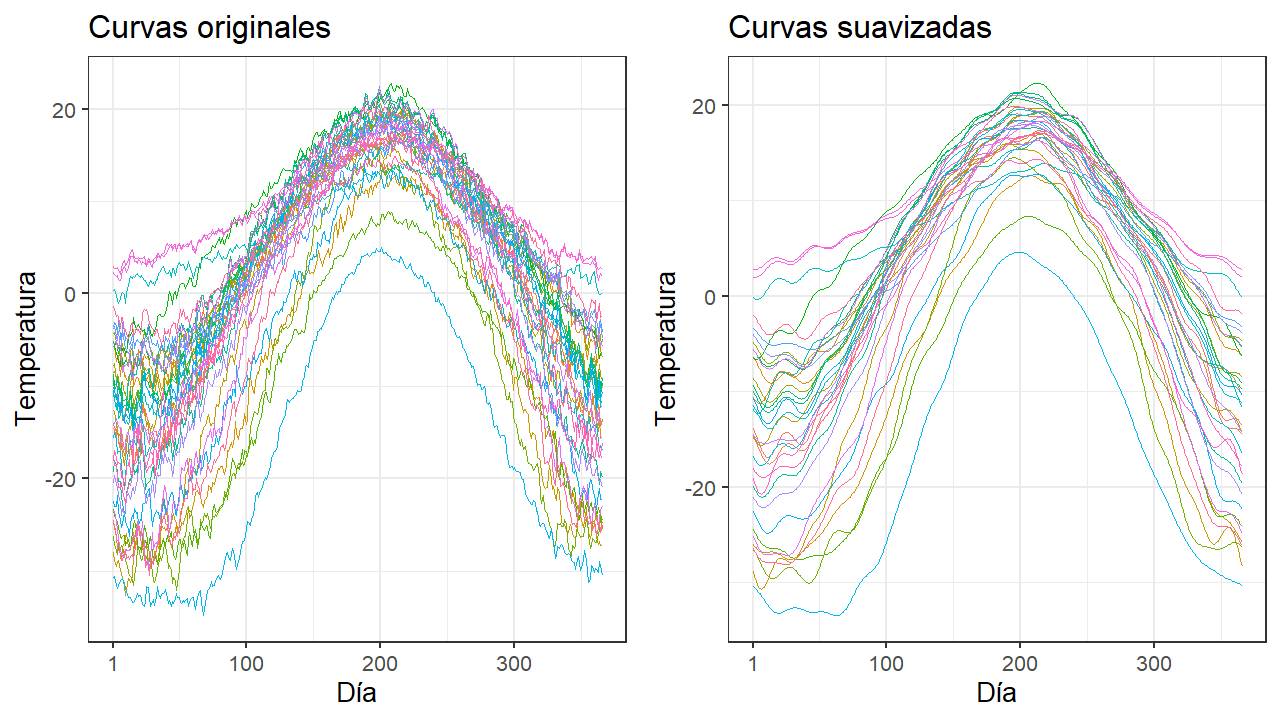
\includegraphics[width=17.78in]{figuras/otros/suves_fda} \caption{Suavización de curvas.}\label{fig:suaves}
\end{figure}

Usualmente, el intervalo donde una función está definida no es \([-\pi,\pi]\) o \([0,\pi]\); también podría ser un intervalo \([a,b]\) arbitrario, por lo cual la expansión en serie de Fourier queda de la siguiente forma:

\begin{align}
    f(x)=\frac{a_0}{2}+\sum_{k=1}^\infty\left(a_k\cos{\frac{2k\pi x}{b-a}} + b_k\sin{\frac{2k\pi x}{b-a}} \right)
\end{align}

donde, para todo \(k\):

\begin{align}
    a_k&=\frac{2}{b-a}\int_a^bf(x)\cos{\frac{2k\pi x}{b-a}}dx\\
    b_k&=\frac{2}{b-a}\int_a^bf(x)\sin{\frac{2k\pi x}{b-a}}dx
\end{align}

\hypertarget{suavizamiento-de-datos-funcionales-mediante-el-uso-de-bases-b-splines}{%
\subsection*{Suavizamiento de datos funcionales mediante el uso de bases B-splines}\label{suavizamiento-de-datos-funcionales-mediante-el-uso-de-bases-b-splines}}
\addcontentsline{toc}{subsection}{Suavizamiento de datos funcionales mediante el uso de bases B-splines}

Se tiene que, en el caso ``más general'', la estimación del vector de coeficientes \(c\), \({\hat{c}}\) es de la forma:

\begin{align}
    {\hat{c}}=(\Phi'W\Phi)^{-1}\Phi'W'y
\end{align}

donde \(\Phi\) es una matriz de orden \(n \times K\) que contiene los valores de las \(K\) funciones base en los \(n\) puntos de muestra, \(W\) es la matriz de ponderación que permite tener una estructura de covarianza en los residuos, y \(y\) es el vector de los datos discretos a ser suavizados; por tanto, la expresión para el vector de ajuste de los datos es:

\begin{align}
    {\hat{y}}=\Phi(\Phi'W\Phi)^{-1} \Phi'Wy=S_\phi y
\end{align}

donde \(S_\phi\) es el operador proyección correspondiente al sistema de base \(\phi\):

\begin{align}
    S_\phi=\Phi(\Phi'W\Phi)^{-1} \Phi'W.
\end{align}

Dado que en el proceso de suavización se tiene un comportamiento de discontinuidades, calcular las rugosidades es de utilidad para compensar dicho comportamiento en los datos suavizados.

Para medir la rugosidad de una función, la integral del cuadrado de la segunda derivada \([D^2x(t)]^2\) se utiliza:

\begin{align}
    PEN_2(x)=\int[D^2x(s)]^2ds
\end{align}

Para funciones con alta variabilidad, se espera un valor alto de \(PEN_2(x)\), pues su segunda derivada es grande al menos en algún rango de interés. De forma general, la penalización de la rugosidad permite una derivada \(D^mx\) de orden arbitrario (\protect\hyperlink{ref-ramsay}{\textbf{ramsay?}}):

\begin{align}
    PEN_m(x)=\int[D^mx(s)]^2ds
\end{align}

matricialmente, la expresión anterior está dada por:

\begin{align}
    PEN_m(x)=c'Rc
 \end{align} dónde

\begin{align}
    R=\int D^m \phi D^m\phi'.
\end{align}

Ahora bien, añadiendo esta penalización al ajuste por mínimos cuadrados y multiplicando por un parámetro \(\lambda\) de suavizamiento, se obtiene:

\begin{align}
    PENSSE_m(y|c)=(y-\Phi c)'W(y-\Phi c)+\lambda c'Rc
\end{align}

y tomando la derivada con respecto al vector \(c\), se obtiene:

\begin{align}
    -2\Phi'Wy + \Phi' W \Phi c + \lambda R c=0
\end{align}

de done la expresión para el vector de coeficientes estimados \({\hat{c}}\) es:

\begin{align}
    {\hat{c}}=(\Phi W \Phi + \lambda R)^{-1} \Phi' Wy
\end{align}

\hypertarget{elecciuxf3n-de-nuxfamero-de-bases}{%
\subsection{Elección de número de bases}\label{elecciuxf3n-de-nuxfamero-de-bases}}

\hypertarget{detecciuxf3n-de-atuxedpicos}{%
\section{Detección de atípicos}\label{detecciuxf3n-de-atuxedpicos}}

El tratamiento de datos atípicos es un aspecto importante en cualquier análisis estadístico, pese a que los datos atípicos influyen de manera significativa en metodologías estadísticas en varios sentidos, su análisis en datos funcionales ha sido poco abordado (\protect\hyperlink{ref-oviedo}{\textbf{oviedo?}}).

De manera intuitiva, se podría pensar en la estadística multivariante para tratar casos de datos atípicos en muestras de datos funcionales. Desafortunadamente, hay varios motivos por las que la estadística multivariante falla en el caso funcional. La primera es que los datos funcionales son realizaciones de un proceso aleatorio suave medido en un conjunto discreto de tiempo, por lo cual la estructura de correlación temporal es ignorada cuando se utilizan métodos de estadística multivariante. La segunda es que por la naturaleza infinto-dimensional, los métodos de estadística multivariante son afectados por la alta dimensionalidad; es decir, los métodos no son capaces de manejar las situaciones en donde el número de mediciones de una o más variables es más grande que el número de individuos en la muestra. La tercera es que pocas asunciones sobre la distribución son impuestas sobre los conjuntos de datos funcionales, mientras que los métodos mutlivariantes están implícitamente sujetos a poblaciones Gaussianas (\protect\hyperlink{ref-oviedo}{\textbf{oviedo?}}).

Los datos atípicos en un conjunto de datos funcionales pueden surgir principalmente por dos razones. La primera es que las curvas pueden tener graves errores de medición, registro o de digitación; estos errores deben ser identificados y corregidos siempre que sea posible. La segunda es que los datos atípicos pueden ser curvas de datos que expresan la realidad, en el sentido de que no tienen errores graves; sin embargo, no se comportan como el resto de curvas. Por tanto, se considera que una curva es un dato atípico si ha sido generado por un proceso estocástico con diferente distribución que el resto de curvas, las cuales se asumen que son idénticamente distribuidas. Una curva puede ser un dato atípico si esta está significativamente alejada del proceso estocástico o si tiene diferente forma y/o comportamiento del resto de curvas (\protect\hyperlink{ref-oviedo}{\textbf{oviedo?}}).

Para identificar datos atípicos en un conjunto de datos funcionales, se hace uso de la \emph{profundidad funcional}. Este concepto fue originalmente introducido en el análisis multivariante para medir la centralidad de un punto en relación con la nube de puntos; es decir, la profundidad da una forma de ordenar los puntos en un espacio Euclídeo desde el centro hacia el exterior; así, los puntos cercanos al centro tendrán una profundidad más grande (\protect\hyperlink{ref-pinero}{\textbf{pinero?}}). Por otro lado, para datos funcionales, si una curva es un dato atípico, esta curva tendrá una profundidad baja, por lo que para detectar la presencia de datos atípicos funcionales basta analizar las curvas con profundidades más bajas (\protect\hyperlink{ref-oviedo}{\textbf{oviedo?}}). Existen tres medidas principales para calcular la profundidad funcional, las cuales son: \emph{Profundidad de Fraiman y Muniz}, \emph{Profundidad H-modal}, y \emph{Profundidad de proyección aleatoria}. Para mayor detalle revisar (\protect\hyperlink{ref-manuel}{\textbf{manuel?}}).

\hypertarget{medidas-de-profundidad}{%
\subsection{Medidas de profundidad}\label{medidas-de-profundidad}}

El objetivo de profundidad para datos funcionales es medir la centralidad de una curva dada \(z_i\) dento de un conjunto de curvas \(z_1,...,z_n\) generadas por un proceso estocástico \(Z(.)\) con muestra de trayectorias en \(C[a,b]\), el espacio de las funciones continuas definidas en el intervalo \([a,b]\subset \mathbb{R}\); es decir, la idea bajo la profundidad funcional es medir cuánto tiempo un curva permanece en el centro de todo el grupo de trayectorias (\protect\hyperlink{ref-manuel}{\textbf{manuel?}}).

\hypertarget{profundidad-de-fraiman-y-muniz}{%
\subsubsection*{Profundidad de Fraiman y Muniz}\label{profundidad-de-fraiman-y-muniz}}
\addcontentsline{toc}{subsubsection}{Profundidad de Fraiman y Muniz}

Sea \(F_{n,t}(z_i(t))\) la función de distribución acumulada empírica de los valores de las curvas \(z_1(t),...,z_n(t)\) en un punto de tiempo \(t\in [a,b]\) dado, dado por:

\begin{align}
    F_{n,t}(z_i(t))=\frac{1}{n}\sum_{k=1}^n I(z_k(t)\leq z_i(t))
\end{align}

donde \(I(.)\) es la función indicatriz.

La medida de profundidad funcional de \emph{Fraiman y Muniz} de una curva \(z_i\) con respecto al conjunto de curvas \(z_1,...,z_n\), está dada por:

\begin{align}
    FMD_n(z_i)=\int_a^bD_n(z_i(t))dt
\end{align}

donde \(D_n(z_i(t))\) es la profundidad univariante del punto \(z_i(t)\) dada por:

\begin{align}
    D_n(z_i(t))=1-\left|\frac{1}{2}-F_{n,t}(z_i(t))\right|
\end{align}

\hypertarget{profundidad-h-modal}{%
\subsubsection*{Profundidad H-modal}\label{profundidad-h-modal}}
\addcontentsline{toc}{subsubsection}{Profundidad H-modal}

Esta medida de profundidad se base en el concepto de moda funcional, definiendo la moda funcional como la curva más densamente rodeada por el resto del conjunto de curvas. Así, la profundidad \emph{h-modal} de una curva \(z_i\), con respecto al conjunto de curvas \(z_1,...,z_n\), está dada por:

\begin{align}
    MD_n(z_i,h)=\sum_{k=1}^n  K\left( \frac{||z_i-z_k||}{h}\right)
\end{align}

\hypertarget{profundidad-de-proyecciuxf3n-aleatoria}{%
\subsubsection*{Profundidad de proyección aleatoria}\label{profundidad-de-proyecciuxf3n-aleatoria}}
\addcontentsline{toc}{subsubsection}{Profundidad de proyección aleatoria}

La idea de esta medida es proyectar cada curva funcional y su primera derivada a través de una dirección aleatoria, definiendo un punto en \(\mathbb{R}^2\), luego, el valor de la profundidad en \(\mathbb{R}^2\), da un orden de puntos proyectados. Si se trabaja con un gran número de proyecciones aleatorias, el valor medio de profundidad de los puntos proyectados define la profundidad para datos funcionales. Así, dado un conjunto de curvas \(z_1,...,z_n\) y una dirección \(\nu\) que pertenece a un proceso independiente direccional \(V(.)\), así la proyección de \(z_i\) a través de la dirección \(\nu\), está dada por:

\begin{align}
    T_{i,\nu}=\langle \nu,z_i \rangle=\int_a^b \nu(t)z_i(t)dt
\end{align}

de manera similar, \(T_{i,\nu}'\)es la proyección de la derivada de \(z_i\) a través de la dirección \(\nu\), obteniendo así el par \((T_{i,\nu},T_{i,\nu}')\) que es un punto en \(\mathbb{R}^2\). Para \(P\) direcciones aleatorias independientes, la profundidad de proyección aleatoria de una curva \(z_i\) está definida por:

\begin{align}
    RPD_n(z-I)=\frac{1}{P}\sum_{p=1}^P D_n((\langle\nu_{p},z_i \rangle),\langle\nu_p, z_{i}'\rangle), h)
\end{align}

donde \(D_n\) es cualquier profundidad definida en \(\mathbb{R}^2\) de los puntos \((\langle\nu_p,z_i \rangle,\langle\nu_p,z_i' \rangle) \in \mathbb{R}^2\) (\protect\hyperlink{ref-manuel}{\textbf{manuel?}}). Para la visualización de datos atípicos se han desarrollado varias herramientas gráficas, principalmente propuestas para el caso univariante; sin embargo, para el caso multivariante han sido poco desarrolladas (\protect\hyperlink{ref-dai}{\textbf{dai?}}).

\hypertarget{gruxe1fico-de-magnitudes-y-formas}{%
\subsection{Gráfico de Magnitudes y Formas}\label{gruxe1fico-de-magnitudes-y-formas}}

Una de la herramientas gráficas usadas es el \textbf{MS-Plot} o \textbf{Gráfico de Magnitudes y Formas} propuesto por (\protect\hyperlink{ref-dai}{\textbf{dai?}}), el cual se basa en el marco de la periferia funcional direccional, que mide la centralidad de los datos funcionales considerando el nivel y la dirección de sus desviaciones de la región central.\textbackslash{}

\textbf{Periferia Funcional Direccional}\textbackslash{}

Teniendo en cuenta que la externalidad es la medida, grado o cualidad de ser atípico; a este concepto se añade el de dirección, ya que la dirección de externalidad es crucial para describir la centralidad de datos funcionales multivariantes.

De manera formal, la externalidad direccional de un dato escalar está definida por:

\begin{align}
    O(Y,F_Y)=\left\{\frac{1}{d(Y,F_Y)-1}\right\}v,\quad d(Y,F_Y)>0
\end{align}

donde \(F_Y\) es la distribución de una variable aleatoria, \(d\) es una medida convencional de profundidad, y \(v\) es el vector unitario que va desde la mediana de \(F_Y\) a \(Y\). Asumiendo que \(Z\) es la única mediana de \(F_Y\) para la medida de profundidad \(d\), \(v\) puede expresarse como:

\begin{align}
    v=\frac{Y-Z}{||Y-Z||}
\end{align}

donde \(||.||\) es la norma \(L_2\).

Ahora bien, si \(X\) es una función p-dimensional definida en un dominio \(\mathcal{I}\), a partir de la distribución de los datos funcionales \(F_X\), para cada punto fijado \(t \in \mathcal{I}\), \(F_{X(t)}\) es la función de distribución de \(X(t)\) con dimensión \(p\). De esta forma, se definen tres medidas de externalidad direccional para datos funcionales:

\begin{itemize}
    \item[1)] Media de externalidad direccional:
    
  \begin{align}
        MO(X,F_X)=\int_{\mathcal{I}}O(X(t),F_{X(t)})w(t)dt
    \end{align}
    
  \item[2)] Variación de externalidad direccional:
    
  \begin{align}
        VO(X,F_{X})=\int_{\mathcal{I}} ||O(X(t),F_{X(t)})-MO(X,F_{X})||^2 w(t) dt
    \end{align}
    
  \item[3)] Externalidad direccional funcional:
    
  \begin{align}
        F0(X,F_X)=\int_{\mathcal{I}}||O(X(t),F_{X(t)})||^2w(t)dt
    \end{align}
    
\end{itemize}

donde \(w(t)\) es una función de peso definida en \(\mathcal{I}\), la cual puede ser constante o proporcional a la variación local en cada punto de diseño; en particular, se usa \(w(t)=\{\lambda(\mathcal{I})\}^{-1}\), donde \(\lambda(.)\) es la medida de Lebesgue.

Las tres medidas anteriores de externalidad pueden escribirse en una sola ecuación de la siguiente manera:

\begin{align}
    FO=||MO||^2 +VO
\end{align}

La ecuación anterior realiza una descomposición total de la externalidad funcional \(\textbf{(FO)}\) en dos términos: la magnitud de externalidad (\(||\textbf{MO}||\)) y la cantidad de variación de externalidad direccional \(\textbf{(VO)}\). Esta descomposición permite una gran flexibilidad para describir la centralidad de un conjunto de datos funcionales y para identificar curvas potencialmente atípicas (\protect\hyperlink{ref-dai}{\textbf{dai?}}). \textbackslash{}

\textbf{MS-Plot}\textbackslash{}

El \textbf{\textit{MS-Plot}} es un gráfico de dispersión de puntos, \((M0',VO)'\), para un grupo de datos funcionales. Cuando la dimensión es más grande que dos, se usa \((||MO||,VO)'\), la cual representa la magnitud general de externalidad y la forma de externalidad sin información de la dirección (\protect\hyperlink{ref-dai}{\textbf{dai?}}).

De las definiciones de MO Y VO, se esperaría que:

\begin{itemize}
\item
  Las curvas centrales se asignen a la región central baja del MS-Plot; es decir, \(||MO||\) pequeño y VO pequeño.
\item
  Valores atípicos desplazados se sitúan en la región inferior; es decir, \(||MO||\) grande y VO pequeño, y las diferentes direcciones de MO indican las diferentes direcciones de sus desplazamientos.
\item
  Los valores atípicos aislados, que están en una pequeña parte del espacio de soporte, se asignan a la región superior central; es decir, \(||MO||\) pequeño y VO grande.
\item
  Los puntos en la región superior exterior corresponden a las curvas que son sustancialmente atípicas tanto en magnitud como en forma; es decir, \(||MO||\) grande y VO grande.
\end{itemize}

\hypertarget{anova-para-datos-funcionales}{%
\section{ANOVA Para datos funcionales}\label{anova-para-datos-funcionales}}

En la práctica se vuelve un problema decidir si existen o no diferencias en el proceso de interés cuando varían condiciones que pueden afectarlo. Este problema se suele abordar mediante un modelo que supone la existencia de una función base que describe la evolución típica del proceso estudiado, suponiendo que los datos con los que se trabaja se han obtenido agregando variaciones aleatorias a esta función. Entonces, este problema se convierte en un tipo de problema de ANOVA funcional (\protect\hyperlink{ref-cuesta}{\textbf{cuesta?}}).

Existen varios procedimientos para tratar problemas de tipo ANOVA. En el presente trabajo se tratará el problema de \emph{one-way} ANOVA para datos funcionales univariantes, conocido también como el problema de la \emph{prueba de k-muestras}.

\hypertarget{one-way-anova}{%
\subsection{One-Way ANOVA}\label{one-way-anova}}

Este problema puede ser formulado de la siguiente manera:

\begin{itemize}
\item
  Sea \(Z_{i1}(t), Z_{i2}(t),..,Z_{in_i}(t),\ i=1,...,k\), donde \(k\) hace referencia a los \(k\) grupos de funciones aleatorias definidas sobre un intervalo finito \(T=[a,b]\) dado.
\item
  Sea \(SP(m,\gamma)\) un proceso estocástico con función de media \(m(t),\ t\in T\) y función de covarianza \(\gamma(s,t), st,t\in T\).
\item
  Asumiendo que \(Z_{i1}(t), Z_{i2}(t),..,Z_{in_i}(t)\) son \(SP(m_i,\gamma),i=1,..,k\) i.i.d.
\end{itemize}

Es interesante comprobar la igualdad de las \(k\) funciones de media; es decir:

\begin{align}
    H_0:m_1(t)&=....=m_k(t),\ t\in T\\
    H_a:m_1(t)&\neq....\neq m_k(t),\ t\in T
\end{align}

A continuación se presentan varias pruebas para este tipo de ANOVA.

\hypertarget{cs-test}{%
\subsubsection*{CS-Test}\label{cs-test}}
\addcontentsline{toc}{subsubsection}{CS-Test}

El siguiente estadístico fue propuesto en (\protect\hyperlink{ref-cuevas}{\textbf{cuevas?}}):

\begin{align}
    V_n=\sum_{1\leq i<j\leq k} n_i\int_T ({\bar{Z_i}}(t)-{\bar{Z_j}}(t))^2dt
\end{align}

Bajo la hipótesis nula y la asunción de que :

\begin{align}
 n_i,n \to \infty \quad \text{tal que}\quad  \dfrac{n_i}{n}\to p_i >0,\ i=1,...,k
\end{align}

se demuestra que la distribución aproximada de \(V_n\) es la del estadístico:

\begin{align}
    V=\sum_{1\leq i<j\leq k} n_i\int_T \left(\bar{Y_i}(t)-\sqrt{\frac{p_i}{p_j}}Y_j(t)\right)^2dt
\end{align}

donde \(Y_1(t),...,Y_k(t)\) son procesos Gaussianos independientes de media cero y función de covarianza \(\gamma(s,t)\). El valor crítico empírico se calcula mediante remuestreo sobre \(Y_i(t),i=1,..,k\) de un proceso Gaussiano con media cero y función de covarianza \({\hat{\gamma}}\), definida por:

\begin{align}
    {\hat{\gamma}}(s,t)&=\frac{1}{n-k}\sum_{i=1}^k\sum_{j=1}^{n_i}(Z_{ij}(s)-\bar{Z_i}(s))(Z_{ij}(t)-\bar{Z_i}(t))
\end{align}

Para el caso heterocedástico y mediante el cálculo del valor crítico empírico, el valor p de \(V_n\) puede calcularse como en el caso anterior, mediante procesos Gaussianos independientes con funciones de covarianza dadas por:

\begin{align}
    {\hat{\gamma_i}}(s,t)=\frac{1}{n_i-1}\sum_{j=1}^{n_i}(Z_{ij}(s)-\bar{Z_i}(s))(Z_{ij}(t)-\bar{Z_i}(t))
\end{align}

\hypertarget{prueba-basadas-en-la-norma-mathcall2}{%
\subsubsection*{\texorpdfstring{Prueba basadas en la norma \(\mathcal{L}^2\)}{Prueba basadas en la norma \textbackslash mathcal\{L\}\^{}2}}\label{prueba-basadas-en-la-norma-mathcall2}}
\addcontentsline{toc}{subsubsection}{Prueba basadas en la norma \(\mathcal{L}^2\)}

Este test usa el siguiente estadístico:

\begin{align}
    S_n=\int_T SSR_n(t)dt 
\end{align}

donde:

\begin{align}
     SSR_n(t)&=\sum_{i=1}^k n_i(\bar{Z}_i(t)-\bar{Z}(t))^2\\
     \bar{Z}(t)&=\frac{1}{n}\sum_{i=1}^k \sum_{j=1}^{n_i}Z_{ij}(t)\\
     \bar{Z}_i(t)&=\frac{1}{n_i}\sum_{j=1}^{n_i}Z_{ij}(t)
 \end{align}

Bajo la hipótesis nula, se tiene que \(S_n\sim \beta \chi_d^2\) aproximadamente, donde:

\begin{align}
    \beta &=\frac{tr(\gamma^{\otimes 2})}{tr(\gamma)},\\
    d&=(k-1)\kappa,\\
    \kappa&=\frac{tr^2(\gamma)}{tr(\gamma^{\otimes 2})},\\
    \gamma^{\otimes 2}(s,t)&=\int_T \gamma(s,u)\gamma(u,t)du.
\end{align}

Esta distribución aproximada es usada para calcular el p-valor de \(S_n\); es decir, \(P(\chi_d^2\geq S_n/\beta)\) o su valor crítico \(\beta\chi_d^2(1-\alpha)\). Los parámetros \(\beta\) y \(\kappa\) son estimados con base en los datos funcionales por el método de \textit{naive} o el método de \textit{reducción de sesgo}.

Utilizando el método naive, y con el estimador \({\hat{\gamma}}(s,t)\), se tiene que:

\begin{align}
    {\hat{\beta}}&=\frac{tr({\hat{\gamma}}^{\otimes 2})}{tr({\hat{\gamma}})},\\
    {\hat{d}}&=(k-1){\hat{\kappa}},\\
    {\hat{\kappa}}&=\frac{tr^2({\hat{\gamma}})}{tr({\hat{\gamma^{\otimes 2}}})}.
\end{align}

Utilizando el método de reducción de sesgo, se tiene que:

\begin{align}
    {\hat{\beta}}&=\frac{{\widehat{tr(\gamma^{\otimes 2})}}}{tr({\hat{\gamma}})},\\
    {\hat{d}}&=(k-1){\hat{\kappa}},\\
    {\hat{\kappa}}&=\frac{{\widehat{tr^2(\gamma)}}}{{\widehat{tr(\gamma^{\otimes 2}})}},\\
    {\widehat{tr(\gamma^{\otimes 2})}}&=\frac{(n-k)^2}{(n-k-1)(n-k+2)}\left(tr({\hat{\gamma}^{\otimes 2}})-\frac{tr^2({\hat{\gamma}})}{n-k} \right),\\
    {\widehat{tr^2(\gamma)}}&=\frac{(n-k)(n-k+1)}{(n-k-1)(n-k+2)}\left(tr^2({\hat{\gamma}})-\frac{2tr({\hat{\gamma}}^{\otimes 2})}{n-k+1}\right).
\end{align}

\hypertarget{prueba-f}{%
\subsubsection*{Prueba F}\label{prueba-f}}
\addcontentsline{toc}{subsubsection}{Prueba F}

Este test usa el estadístico:

\begin{align}
    F_n&=\frac{\int_T SSR_n(t)dt/(k-1)}{\int_T SSE_n(t)dt/(n-k)}\\
    SSE_n(t)&=\sum_{i=1}^k\sum_{j=1}^{n_i}(Z_{ij}(t)-\bar{Z}_i(t))^2
\end{align}

Bajo la hipótesis nula, se tiene que \(F_n \sim F_{d_1,d_2}\) aproximadamente, donde \(d_1=(k-1)\kappa\) y \(d_2=(n-k)\kappa\). De manera similar, la distribución aproximada de la prueba \textit{F} puede ser usada para calcular el p-valor de \(F_n\) o su valor crítico; y el parámetro \(\kappa\) puede ser estimado por el método naive o el método de reducción de sesgo.

Cuando las muestras nos son Gaussianas o son pequeñas, estas pruebas no son utilizadas; en este caso, las versiones bootstrap de estas pruebas son usadas para calcular el p-valor de \(S_n\) y \(F_n\) (\protect\hyperlink{ref-gorgi}{\textbf{gorgi?}}).\textbackslash{}

\hypertarget{prueba-basada-en-representaciuxf3n-de-funciones-base}{%
\subsubsection*{Prueba basada en representación de funciones base}\label{prueba-basada-en-representaciuxf3n-de-funciones-base}}
\addcontentsline{toc}{subsubsection}{Prueba basada en representación de funciones base}

Se puede utilizar una función de representación de base para obtener una prueba más robusta.

Asumiendo que se trabaja con \(k\) grupos de un proceso estocástico \(Z_{ij}\in L_2(T), i=1...,k,j=1,...,n_i\) y sea \(\{\phi_l\}\) una base ortonormal de \(L_2(T)\).

Esta prueba usa el siguiente estadístico:

\begin{align}
    F=\frac{\frac{1}{k-1}\sum_{i=1}^k n_i||\bar{Z}_i-\bar{Z}||^2}{\frac{1}{n-k}\sum_{i=1}^k\sum_{j=1}^{n_i} ||Z_{ij}-\bar{Z_i}||^2}
\end{align}

donde el proceso estocástico, la media funcional muestral y media funcional grupal, escrita en notación matricial a partir de la representación en la base \(\phi\), están definidos de la siguiente manera:

\begin{align}
    Z_{ij}(t)&=c'_{ij}\phi(t),\\
    \bar{Z}(t)&=\frac{1}{n}\sum_{i=1}^k\sum_{j=1}^{n_i} c'_{ij}\phi(t), \quad \forall t\in T\\
    \bar{Z}_i(t)&=\frac{1}{n_i}\sum_{j=1}^{n_i}c'_{ij}\phi(t)
\end{align}

para todo \(t\in T\).

El numerador del estadístico \textit{F}, mide la variabilidad externa entre las diferentes muestras, mientras que el denominador mide la variabilidad interna dentro de las muestras (\protect\hyperlink{ref-cuevas}{\textbf{cuevas?}}).

\hypertarget{introducciuxf3n-a-la-estaduxedstica-esepacial-funcional}{%
\chapter{Introducción a la estadística esepacial funcional}\label{introducciuxf3n-a-la-estaduxedstica-esepacial-funcional}}

\hypertarget{proceso-espacial-funcional}{%
\section{Proceso Espacial Funcional}\label{proceso-espacial-funcional}}

\hypertarget{datos-funcionales-espaciales}{%
\section{Datos funcionales espaciales}\label{datos-funcionales-espaciales}}

\hypertarget{variable-regionalizada-funcional}{%
\section{Variable Regionalizada Funcional}\label{variable-regionalizada-funcional}}

\hypertarget{funciuxf3n-de-distribuciuxf3n-conjunta-funcional}{%
\section{Función de Distribución Conjunta Funcional}\label{funciuxf3n-de-distribuciuxf3n-conjunta-funcional}}

\hypertarget{funciuxf3n-de-media-funcional}{%
\section{Función de Media Funcional}\label{funciuxf3n-de-media-funcional}}

\hypertarget{funciuxf3n-de-varianza-funcional}{%
\section{Función de varianza Funcional}\label{funciuxf3n-de-varianza-funcional}}

\hypertarget{funciuxf3n-de-covarianza-funcional}{%
\section{Función de Covarianza Funcional}\label{funciuxf3n-de-covarianza-funcional}}

\hypertarget{funciuxf3n-de-correlaciuxf3n-o-correlograma-funcional}{%
\section{Función de correlación o Correlograma Funcional}\label{funciuxf3n-de-correlaciuxf3n-o-correlograma-funcional}}

\hypertarget{funciuxf3n-de-semi-variograma-funcional}{%
\section{Función de semi-variograma Funcional}\label{funciuxf3n-de-semi-variograma-funcional}}

\hypertarget{estacionariedad-de-funciones-aleatorias-1}{%
\section{Estacionariedad de Funciones Aleatorias}\label{estacionariedad-de-funciones-aleatorias-1}}

\hypertarget{no-estacionariedad-de-funciones-aleatorias-1}{%
\section{No estacionariedad de Funciones Aleatorias}\label{no-estacionariedad-de-funciones-aleatorias-1}}

\hypertarget{correlaciuxf3n-espacial-funcional}{%
\section{Correlación Espacial Funcional}\label{correlaciuxf3n-espacial-funcional}}

\hypertarget{uxedndices-de-correlaciuxf3n-espacial}{%
\section{Índices de correlación espacial}\label{uxedndices-de-correlaciuxf3n-espacial}}

\hypertarget{uxedndice-de-moran-funcional}{%
\subsection{Índice de Moran funcional}\label{uxedndice-de-moran-funcional}}

\hypertarget{uxedndice-de-geary-funcional}{%
\subsection{Índice de Geary funcional}\label{uxedndice-de-geary-funcional}}

\hypertarget{agrupaciuxf3n}{%
\chapter{Agrupación}\label{agrupaciuxf3n}}

De manera empírica, agrupación significa encontrar grupos en un conjunto de datos. La primera agrupación en la historia fue de tipo jerárquico, cuando Aristóteles clasificó a los seres vivos. El análisis de agrupación ha sido desarrollado en diferentes campos y con diversas aplicaciones (\protect\hyperlink{ref-hand}{\textbf{hand?}}).

En el análisis de agrupación el objetivo es examinar datos que no contienen etiquetas, para luego encontrar agrupaciones de los datos; se debe tener en cuenta que se desconoce el número de grupos. Esta metodología es una forma de aprendizaje no supervisado; es decir, no se utilizan datos de entrenamiento. (\protect\hyperlink{ref-andrew}{\textbf{andrew?}}).

Formalmente, si se tiene un conjunto de datos, \(D=\{z_1,z_2,...,z_n\}\), el cual contiene \(n\) datos, la tarea de los métodos de agrupación es asignarlos a \(K\) subconjuntos disjuntos de \(D\), denotados por \(C_1,C_2,...,C_K\) (\protect\hyperlink{ref-hand}{\textbf{hand?}}). Estos métodos con frecuencia se utilizan como un paso preliminar en la exploración de datos para identificar patrones que tengan una interpretación útil para el usuario (\protect\hyperlink{ref-Jaque}{\textbf{Jaque?}}).

\hypertarget{algoritmos-de-agrupaciuxf3n}{%
\section{Algoritmos de agrupación}\label{algoritmos-de-agrupaciuxf3n}}

Algoritmo 1 Algoritmo 2 Algoritmo 3 Algoritmo 4

\hypertarget{agrupaciuxf3n-datos-multivariantes-apuxe9ndice}{%
\section{Agrupación: Datos Multivariantes (apéndice)}\label{agrupaciuxf3n-datos-multivariantes-apuxe9ndice}}

\hypertarget{agrupaciuxf3n-datos-funcionales}{%
\section{Agrupación: Datos Funcionales}\label{agrupaciuxf3n-datos-funcionales}}

Como se mencionó, el objetivo principal del análisis de agrupación es construir grupos homogéneos de observaciones que representen realizaciones de alguna variable aleatoria \(Z\), y se busca que las observaciones asignadas a los grupos sean similares entre ellas y lo más diferente posible de las observaciones asignadas a otros grupos (\protect\hyperlink{ref-joan}{\textbf{joan?}}). En el espacio finito dimensional, \(Z\) es un vector aleatorio con valores en \(\mathbb{R}^p\), \(Z=(Z_1,...,Z_p), p\geq 1\). Un caso particular es cuando las variables aleatorias toman valores en un espacio infinito dimensional, usualmente un espacio de funciones definidas en algún conjunto continuo \(\mathcal{T}\); de esta forma los datos son representados por medio de curvas y la variable aleatoria que corresponde a los datos es un proceso estocástico \(Z=\{Z(t),t \in \mathcal{T}\}\). En la actualidad este tipo de datos son más fáciles de observar y se han desarrollado herramientas para poderlos almacenar y procesar (\protect\hyperlink{ref-Jaque}{\textbf{Jaque?}}).

Se conocen cuatro metodologías para la agrupación de datos funcionales, las cuales son:

\begin{itemize}
\item
  Métodos de datos en bruto: Estos métodos consisten en agrupar directamente las curvas sobre la base de sus puntos de evaluación.
\item
  Métodos de filtrado: Estos métodos realizan la aproximación de las curvas en alguna base de funciones y luego realizan la agrupación utilizando los coeficientes de la expansión en la base.
\item
  Métodos adaptativos: Estos métodos consideran que la representación de un dato funcional depende del grupo, y se realiza simultáneamente la reducción de dimensión y la agrupación.
\item
  Métodos con base en distancias: Estos métodos usan algoritmos de agrupación con base en distancias específicas para datos funcionales.
\end{itemize}

En el presente trabajo se hará uso de los métodos de filtrado y los métodos basados en distancias.

\hypertarget{muxe9todos-de-datos-en-bruto}{%
\subsection{Métodos de datos en bruto}\label{muxe9todos-de-datos-en-bruto}}

Este primer enfoque, uno de los más sencillos, consiste en utilizar directamente la discretización de las funciones en algunos puntos de tiempo; en este caso no es necesario reconstruir la forma funcional de los datos, debido al gran tamaño de la discretización, por lo cual se requiere utilizar métodos de agrupación para datos vectoriales de alta dimensión.

Existen métodos que realizan agrupación extrayendo las observaciones a partir de datos con ruido, por lo cual se espera pérdidas de información; incluso curvas observadas en diferentes puntos de evaluación pueden no ser tomadas en cuenta por este método. Por otro lado, existen métodos que realizan la agrupacióncon base en la distribución de probabilidad de las observaciones discretas de las curvas en cada intervalo de alguna partición de algún conjunto continuo \(\mathcal{T}\). En general, estos métodos tienen la ventaja de que no dependen de ninguna asunción sobre de la naturaleza de los datos, puesto que la expansión de base no se utiliza (\protect\hyperlink{ref-Jaque}{\textbf{Jaque?}}).

\hypertarget{muxe9todos-de-filtrado}{%
\subsection{Métodos de filtrado}\label{muxe9todos-de-filtrado}}

Este método consiste de dos etapas para la agrupación de datos funcionales. La primera hace referencia al método de filtrado, el cual reduce la dimensión de los datos, pues consiste generalmente en aproximar las curvas utilizando una base finita de funciones; esta base puede ser de tipo B-splines, Fourier o Wavelets; otra técnica de reducción de dimensión es el análisis de componentes principales funcionales (FACP). La segunda etapa consiste en que a partir de los coeficientes de la base de expansión o de los \emph{scores} de los componentes principales, se aplican algoritmos habituales de agrupación para determinar los grupos (\protect\hyperlink{ref-Jaque}{\textbf{Jaque?}}).

Se debe tener en cuenta que el método de filtrado tiene algunos inconvenientes; uno de ellos es que si las curvas son medidas en diferentes puntos de tiempo, la varianza de la estimación de los coeficientes de base es distinto para cada individuo. Para conjuntos de datos dispersos, varios coeficientes de base podrían tener varianza infinita, haciendo imposible obtener estimaciones razonables (\protect\hyperlink{ref-sugar}{\textbf{sugar?}}).

\hypertarget{muxe9todos-adaptativos}{%
\subsection{Métodos adaptativos}\label{muxe9todos-adaptativos}}

Contrario al método de filtrado en donde las curvas son aproximadas en una base finita de funciones y sus curvas son identificadas mediante los coeficientes de expansión de la base, en este método en lugar de tratar los coeficientes como parámetros, estos son considerados variables aleatorias con una distribución de probabilidad de un grupo específico. Estos métodos se dividen en dos grupos, los que modelan los scores del FPCA y los que modelizan directamente los coeficientes de expansión de una base finita de funciones (\protect\hyperlink{ref-Jaque}{\textbf{Jaque?}}).

\hypertarget{clasificaciuxf3n-basados-en-modelos}{%
\subsection{Clasificación basados en modelos}\label{clasificaciuxf3n-basados-en-modelos}}

En el marco multivariante, este método utiliza la técnica de agrupación basada en modelos; es decir, se asume que las observaciones \(z_1,...,z_n\) son generadas de acuerdo a una distribución mixta con \(G\) componentes. Sea \(f_k(z,\theta_k)\) la densidad correspondiente al \emph{k-ésimo} grupo con parámetro \(\theta_k\), y sea \(y_i=(y_{i1},...,y_{iG})\) un vector que indica la pertenencia a un grupo para la \emph{i-ésima} observación donde \(y_{ik}=1\) si \(z_i\) es un miembro del \emph{k-ésimo} grupo y \(0\) caso contrario. Los \(y_i\) son desconocidos y generalmente son tratados con uno de los dos siguientes enfoques: \emph{clasificación por verosimilitud} o \emph{verosimilitud mixta}.

En el primer enfoque, los \(y_i\) son vistos como parámetros y el modelo es ajustado para maximizar la verosimilitud:

\begin{align*}
    L_c(\theta_1,...,\theta_G;y_1,...,y_n|z_1,...,z_n)=\prod_{i=1}^n {f_{y_i}(z_i|\theta_{y_i})}
\end{align*}

donde \(f_{k}(z|\theta_k)\) es una normal multivariante con matriz identidad como covarianza; este enfoque produce una solución por \emph{k-medias} (\protect\hyperlink{ref-sugar}{\textbf{sugar?}}).

Por otro lado, el segundo enfoque también considera \(f_k(z,\theta_k)\) como una normal multivariante y con matriz identidad como covarianza; sin embargo, puede ocurrir que los miembros de algún grupo pueden ser tratados como datos faltantes, donde \(y_i\) es una multinomial con parámetros \((\pi_1,...,\pi_G)\) y \(\pi_k\) es la probabilidad de que una observación pertenezca al \emph{k-ésimo} grupo; entonces, los parámetros son estimados maximizando lo siguiente:

\begin{align*}
    L_M(\theta_1,...,\theta_G;\pi_1,...,\pi_n|z_1,...,z_n)=\prod_{i=1}^n \sum_{k=1}^G\pi_k f_{y_i}(z_i|\theta_{y_k})
\end{align*}

La principal diferencia entre estos dos enfoques es que en el primero, cada punto se asigna a un único grupo, mientras que en el segundo a cada punto se le asigna a una probabilidad originada en cada grupo y así influye en la estimación de todos los parámetros (\protect\hyperlink{ref-sugar}{\textbf{sugar?}}).

\hypertarget{muxe9todo-adaptativo-de-agrupaciuxf3n-usando-coeficientes-de-bases-de-expansiuxf3n}{%
\subsection{Método adaptativo de agrupación usando coeficientes de bases de expansión}\label{muxe9todo-adaptativo-de-agrupaciuxf3n-usando-coeficientes-de-bases-de-expansiuxf3n}}

El algoritmo \textbf{fclust} es el primer algoritmo de agrupación de este tipo y fue propuesto por (\protect\hyperlink{ref-sugar}{\textbf{sugar?}}), donde consideran que los coeficientes de la base de expansión tipo spline de las curvas se distribuyen de acuerdo a una mezcla de distribuciones Gaussianas con media específica para cada grupo \(\mu_k\) y una varianza común \(\Sigma\); es decir:

\begin{align*}
    \alpha_i \sim \mathcal{N}(\mu_k,\Sigma)
\end{align*}

A diferencia de los métodos de filtrado, en el cual los coeficientes de la base de expansión son considerados fijos, aquí son considerados como variables aleatorias, que además permite proceder eficientemente con una muestra de curvas dispersa (\protect\hyperlink{ref-Jaque}{\textbf{Jaque?}}).

\hypertarget{muxe9todo-adaptativo-de-agrupaciuxf3n-usando-fpca}{%
\subsection{Método adaptativo de agrupación usando FPCA}\label{muxe9todo-adaptativo-de-agrupaciuxf3n-usando-fpca}}

Utilizando la noción de densidad de probabilidad para variables aleatorias funcionales desarrollada en (\protect\hyperlink{ref-delagua}{\textbf{delagua?}}) y asumiendo una distribución Gaussiana de los componentes principales y definiendo las técnicas de agrupación basadas en el modelo combinado dador por:

\begin{align*}
    f_Z^{(q)}(z;\theta)=\sum_{k=1}^{q_k} \pi_k\prod_{j=1}^{q_k} f_{C_{j{|Y_k=1}}}(c_{jk}(z);\lambda_{jk})
\end{align*}

donde \(\theta=(\pi_{k},\lambda_{1k},...,\lambda_{q_{k}k})_{1\leq k \leq K}\) son los parámetros del modelo referentes a las proporciones de los grupos y las varianzas de los componentes principales y \(q_k\) es el orden de la densidad de probabilidad específica para el grupo \(k\) (\protect\hyperlink{ref-Jaque}{\textbf{Jaque?}}). En (\protect\hyperlink{ref-cristian}{\textbf{cristian?}}) se desarrolló el modelo denominado \emph{funclust} y los scores \(c_{jk}(z)\) de \(Z\) son calculados en cada grupo (\protect\hyperlink{ref-Jaque}{\textbf{Jaque?}}). Si el FPCA no fuera calculado para cada grupo, tales métodos corresponden a una agrupacióncon base en modelos con probabilidades Gaussianas aplicados a los scores del FPCA y podrían ser considerados como métodos de filtrado.

Estos métodos son importantes puesto que asumiendo una distribución de probabilidad de los coeficientes de la base de expansión permiten tomar en cuenta la incertidumbre gracias a la reconstrucción de los datos funcionales (\protect\hyperlink{ref-Jaque}{\textbf{Jaque?}}).

\hypertarget{muxe9todos-basados-en-distancia}{%
\subsection{Métodos basados en distancia}\label{muxe9todos-basados-en-distancia}}

Estos métodos también son conocidos como métodos no paramétricos y se dividen en dos categorías, la primera agrupa los métodos que hacen uso de distancias o disimilitudes específicas, mientras que la segunda hace uso de heurísticas.

\hypertarget{muxe9todos-que-usan-distancias}{%
\subsubsection*{Métodos que usan distancias}\label{muxe9todos-que-usan-distancias}}
\addcontentsline{toc}{subsubsection}{Métodos que usan distancias}

Estos métodos aplican técnicas de agrupación no paramétrica como el método k-medias o el método jerárquico, los cuales consideran distancias específicas o disimilitudes entre curvas. Para este propósito se utiliza una métrica basada en derivadas que mide la proximidad en las curvas \(z_i\) y \(z_i'\) mediante la siguiente expresión:

\begin{align*}
    d_q(z_i,z_i')^2=\int\left( z_i^{(q)}(t)-z_{i'}^{(q)}(t)\right)^2dt
\end{align*}

donde \(z^{(q)}\) denota la \emph{q-ésima} derivada de \(z\) y \(d_0(z,0)\) es la norma \(\mathcal{L}^2\) (\protect\hyperlink{ref-ferraty}{\textbf{ferraty?}}). Si el cálculo de \(d_0\) se lo realiza utilizando las observaciones discretas de la curva, los métodos no paramétricos son equivalentes a los métodos de agrupación de datos brutos. Por otro lado, si el cálculo de \(d_0\) se lo realiza mediante la representación de las curvas en una base finita, estos métodos son equivalentes a los métodos de filtrado (\protect\hyperlink{ref-Jaque}{\textbf{Jaque?}}).

\hypertarget{muxe9todos-heuruxedsticos}{%
\subsubsection*{Métodos Heurísticos}\label{muxe9todos-heuruxedsticos}}
\addcontentsline{toc}{subsubsection}{Métodos Heurísticos}

Estos métodos proponen usar heurísticas para la agrupación de datos funcionales. En (\protect\hyperlink{ref-herbalife}{\textbf{herbalife?}}) se desarrollaron dos algoritmos de programación dinámica que realizan la agrupación y la estimación de los centros de cada grupo simultáneamente. Por otro lado, en (\protect\hyperlink{ref-yamamoto}{\textbf{yamamoto?}}) se desarrolló un procedimiento para identificar simultáneamente grupos óptimos de funciones y subespacios óptimos para la agrupación; para esto se define una función objetivo como la suma de las distancias entre las observaciones y sus proyecciones más las distancias entre las proyecciones y las medias de los grupos (\protect\hyperlink{ref-Jaque}{\textbf{Jaque?}}).

\hypertarget{agrupaciuxf3n-datos-espaciales}{%
\section{Agrupación: Datos Espaciales}\label{agrupaciuxf3n-datos-espaciales}}

El incremento de los datos espaciales y el uso extendido de bases de este tipo de datos ponen en evidencia la necesidad de generar procesos que permitan la extracción de información espacial; en este sentido se ha desarrollado la minería de datos espaciales, debido a que esta permite descubrir patrones interesantes y previamente desconocidos pero potencialmente útiles (\protect\hyperlink{ref-sumati}{\textbf{sumati?}}). A medida que se dispone de más y más datos sobre un área espacial es deseable identificar las diferentes funciones y papeles que desempeñan las distintas partes de esta área; en particular, un objetivo bastante deseable es identificar regiones homogéneas y descubrir sus características, creando resúmenes de alto nivel para los datos en estudio y obteniendo información valiosa para planificadores, científicos, entre otros (\protect\hyperlink{ref-cesario}{\textbf{cesario?}}).

Los datos espaciales poseen dos atributos distintos: uno espacial y otro no espacial. Los atributos espaciales de este tipo de datos incluyen información relacionada a la ubicación espacial como longitud, latitud, elevación, forma, entre otros. Por otro lado, los atributos no espaciales se utilizan para describir características como nombre, población, tasa de desempleo, entre otros. Se debe tener en cuenta que la información espacial referente a las relaciones entre los datos, tales como la influencia de los datos con los de sus vecinos, usualmente está implícita; por lo cual, para capturar esta información se hace uso de técnicas o instrumentos que la incorporen (\protect\hyperlink{ref-chuek}{\textbf{chuek?}}). Para este propósito se hace uso de las siguientes técnicas:

\begin{itemize}
\item
  Generalizaciones basadas en descubrimiento de conocimiento.
\item
  Métodos de agrupación.
\item
  Medidas de proximidad agregada.
\item
  Reglas de asociación espacial.
\end{itemize}

El presente trabajo se enfocará en los métodos de agrupación. Este clase de métodos han sido desarrollados por la estadística a lo largo del tiempo, en primera instancia se trabajó en una dimensión, y se centraron en la búsqueda de medidas de tendencia, variabilidad o dispersión. Luego se extendió para dos dimensiones, que tratan atributos con media o propiedades modales y variabilidad o dispersión, estos atributos son bidimensionales; en el caso de datos espaciales estas cantidades tiene interpretación como la ubicación del centro del grupo y la dispersión del grupo (\protect\hyperlink{ref-andrew}{\textbf{andrew?}}).

Los métodos clásicos de agrupación utilizados para particionar un conjunto de datos espaciales dan como resultado grupos que espacialmente están mezclados o carecen de sentido (\protect\hyperlink{ref-ambrosi}{\textbf{ambrosi?}}); para dar solución a este problema, se han desarrollado métodos que toman en cuenta la información espacial de los datos; la aplicación de estos incluyen la identificación de áreas con características o factores similares y el objeto de estudio depende del campo de aplicación.

Una solución que ha sido utilizada a lo largo de los años es ponderar las disimilitudes entre las muestras mediante la función de variograma; es decir:

\begin{align*}
    d_{ij}^*=d_{ij}\gamma(h)
\end{align*}

donde \(\gamma(h)\) es el variograma ajustado al variograma empírico \(\hat{\gamma}(h)\); \(d_{ij}\) es la disimilitud entre las muestras \(i\) y \(j\) (\protect\hyperlink{ref-borou}{\textbf{borou?}}).

Por otro lado, en el caso multivariante, en cuanto a similaridad, se tiene que la ponderación está realizada mediante la función de autocovarianza multivariada; es decir:

\begin{align*}
    S^{*2}_{ij}=S_{ij}^2K(h)
\end{align*}

Esta ecuación es más robusta en el sentido de que favorece a la formación de grupos que son espacialmete homogéneos.

Por otro lado, en cuanto a disimilitud y utilizando la función de variograma multivariado se tiene que:

\begin{align*}
    d_{ij}^{*2}=d_{ij}^2\Gamma(h)
\end{align*}

Se debe tener en cuenta que esta última ecuación es un poco más general ya que permite variogramas multivariados sin silla. Ambas ecuaciones se desempeñan adecuadamente cuando el efecto pepita está presente (\protect\hyperlink{ref-borou}{\textbf{borou?}}).

Una vez que los cálculos son realizados para todos los \(i\) y \(j\) el resultado es una matriz de disimilitud modificada \(D^*\) con elementos \(d_{ij}^*\). Esta matriz se utiliza por una amplia variedad de estrategias de clasificación; por ejemplo, el método jerárquico opera directamente en esta matriz, agrupando primero aquellos individuos para los cuales \(d_{ij}^*\) es la menor y luego la menos similar según las reglas del algoritmo en uso. Por otro lado, la agrupación dinámica es más apropiada para agrupar individuos de poblaciones que no presentan estructura jerárquica (\protect\hyperlink{ref-oliver}{\textbf{oliver?}}).

A partir de esta ponderación se pueden aplicar algunos métodos de agrupación que se clasifican de la siguiente forma:

\begin{itemize}
\tightlist
\item
  \textbf{Métodos jerárquicos}
\end{itemize}

Este método agrupa los datos en forma de árboles y generalmete se clasifican en dos tipos de enfoque, uno aglomerativo y otro divisivo.

\begin{itemize}
\item
  \textbf{El enfoque aglomerativo:}
  Utiliza una estrategia ascendente para agrupar los objetos; se fusionan los grupos más pequeños en grupos cada vez más grandes hasta que todos los objetos hayan sido agrupados en uno solo. Los métodos más utilizados son AGNES y DIANA.
\item
  \textbf{El enfoque divisivo:}
  Utiliza una estrategia descendente para agrupar los objetos, en este caso los grupos más grandes se dividen en grupos más pequeños hasta que cada objeto forme un grupo por si mismo. Los métodos más utilizados son: CURE, BIRC Y CHAMALEON (\protect\hyperlink{ref-ritu}{\textbf{ritu?}}).
\item
  \textbf{Métodos de particionamiento.}
\end{itemize}

Los algoritmos de partición organizan los objetos en grupos tales que la dispersión total de cada objeto con respecto a su centro de grupo se minimice. Inicialmente, cada objeto se clasifica como un único grupo; en los siguientes pasos, todos los puntos de datos se reasignan iterativamente a cada grupo hasta que se cumpla un cierto criterio de parada. Bajo este criterio existen los siguientes métodos (\protect\hyperlink{ref-sumati}{\textbf{sumati?}}): algoritmo del vecino más cercano, algoritmo K-medioides, algoritmo K-medias.

\begin{itemize}
\tightlist
\item
  \textbf{Métodos con base en grillas.}
\end{itemize}

Los algoritmos de agrupación con base en grillas primero cuantifican el espacio de agrupación en un número limitado de celdas y luego realizan las operaciones necesarias en la estructura de la grilla, las celdas que contienen más de un cierto número de puntos se tratan como densas, la principal ventaja de este enfoque es su rápido tiempo de procesamiento ya que el tiempo es independiente del número de objetos de datos pero depende del número de celdas. Los métodos más utilizados de este tipo son: STRING, Wave Grupo, Cliqué (\protect\hyperlink{ref-sumati}{\textbf{sumati?}}).

\begin{itemize}
\tightlist
\item
  \textbf{Métodos con base en densidades.}
\end{itemize}

El método considera los grupos como regiones densas de objetos separadas por regiones de baja densidad, que representan el ruido; a diferencia de los métodos de partición se pueden descubrir grupos de manera arbitraria. Los métodos con base en densidades pueden utilizarse para filtrar el ruido y los valores atípicos. Los métodos más utilizados de este tipo son: DBSCAN y OPTICS (\protect\hyperlink{ref-sumati}{\textbf{sumati?}}).

\hypertarget{agrupaciuxf3n-datos-funcionales-con-correlaciuxf3n-espacial}{%
\section{Agrupación: Datos funcionales con correlación espacial}\label{agrupaciuxf3n-datos-funcionales-con-correlaciuxf3n-espacial}}

Como se ha visto a lo largo de este capítulo, los métodos de agrupación se han ido adaptando a las necesidades para tratar los problemas del mundo real. Puesto que se ha ido generalizando esta técnica para trabajar con datos puntuales, luego datos espaciales y datos funcionales; ahora la nueva problemática es extender aun más estos métodos de agrupación para datos funcionales con dependencia espacial. Este es el caso cuando las muestras son funciones observadas en diferentes sitios de una región o cuando estas funciones son observadas sobre un conjunto discreto de tiempo. Si los datos funcionales son espacialmente dependientes, los métodos básicos de agrupación de FDA fallan, ya que la estructura espacial es ignorada dando como resultado grupos en donde las curvas no son similares en forma o comportamiento. Es así que, además de considerar las características individuales en cada una de las curvas, se debe considerar la ubicación espacial de la curva y así agrupar aquellas curvas que son homogéneas no solo con respecto a su forma sino también con respecto a su ubicación espacial (\protect\hyperlink{ref-Romano}{\textbf{Romano?}}).

Para agrupar datos funcionales con correlación espacial se han desarrollado métodos como el dinámico y jerárquico, así como varias formas de capturar la dependencia espacial. En (\protect\hyperlink{ref-Hclust}{\textbf{Hclust?}}) se propuso el método jerárquico y en (\protect\hyperlink{ref-RomanoDIN}{\textbf{RomanoDIN?}}) el método dinámico; ambos métodos utilizan una medida de asociación espacial para resaltar y distinguir la dependencia espacial entre las curvas; esta medida está dada por la función trazo-variograma. Ambos métodos tienen en cuenta la dinámica funcional de las curvas en términos de tiempo y sus relaciones espaciales. El método jerárquico toma en cuenta la dinámica funcional a través de la distancia entre las curvas mediante la norma \(\mathcal{L}^2\), mientras que el método dinámico la considera a través de la distancia euclidiana al cuadrado entre las curvas calculando la función de variograma en cada grupo. No obstante, la dependencia espacial influye de manera diferente en el proceso de agrupación; en el caso jerárquico, la dependencia espacial es considerada por la función de trazo-variograma y en el caso dinámico, esta dependencia es considerada también por el trazo-variograma, pero calculado dentro de cada grupo (\protect\hyperlink{ref-Romano}{\textbf{Romano?}}). Por otro lado en (\protect\hyperlink{ref-Elvira}{\textbf{Elvira?}}) presentan un método para este tipo de datos tomando en cuenta la contribución de cada curva a la variabilidad espacial; de esta forma se define una función de dispersión espacial asociada a cada curva y llevan a cabo la agrupación utilizando el algoritmo k-medias; este algoritmo se basa en la optimización de un criterio de ajuste entre las funciones de dispersión espacial asociadas a cada curva y el representante o centro de los grupos. En el trabajo realizado por (\protect\hyperlink{ref-romanoNP}{\textbf{romanoNP?}}) se extiende la estrategia de agrupación con base en modelos para datos funcionales con correlación espacial; esta estrategia se enfoca en clasificar curvas espacialmente dependientes y obtener un modelo funcional espacial base para cada grupo; el ajuste de estos modelos implica estimar la función trazo-variograma, por lo que proponen un estimador de variograma de kernel.\%no se ha definido lo de kernel

Ahora bien, dado que el objetivo de este trabajo es adaptar el método k-medias para datos funcionales espacialmente correlacionados, se hará uso de la metodología planteada en (\protect\hyperlink{ref-Hclust}{\textbf{Hclust?}}).

\hypertarget{muxe9todo-jeruxe1rquico-para-datos-funcionales-con-correlaciuxf3n-espacial}{%
\subsection{Método jerárquico para datos funcionales con correlación espacial}\label{muxe9todo-jeruxe1rquico-para-datos-funcionales-con-correlaciuxf3n-espacial}}

Suponiendo que \(X_1(t),...,X_n(t)\) es una muestra de curvas definidas en \(t\in T=[a,b]\subseteq \mathbb{R}\) y que además pertenecen al espacio de Hilbert de funciones cuadrado integrables definidas en \([a,b]\); es decir:

\begin{align*}
    L_2(T)=\left\{f: T\to \mathbb{R}: \int_Tf(t)^2<\infty \right\}.
\end{align*}

De igual manera, se asume que las funciones son expandidas en términos de alguna base de funciones como sigue:

\begin{align*}
    X_i(t)=\sum_{l=1}^Ka_{il}B_l(t)=a_i^TB(t),\quad i=1,...,n
\end{align*}

El análisis de agrupación jerárquico funcional es desarrollado como en el enfoque clásico, pero considerando la distancia entre las curvas \(X_i(t)\) y \(X_j(t)\) a través de la norma \(\mathcal{L}^2\); es decir:

\begin{align*}
    d_{ij}=\sqrt{\int_{[a,b]} (X_{i}(t)-X_{j}(t))^2 dt}
\end{align*}

de donde, utilizando la representación de la curva en la base de funciones, se tiene:

\begin{align*}
    d_{ij}&=\sqrt{\int_{[a,b]} ((a_i - a_j)^T B(t)B(t)^T (a_i - a_j) dt}\\\\
   d_{ij} &=\sqrt{(a_i-a_j)^T W (a_i - a_j)}
\end{align*}

donde:

\begin{align*}
    W=\int_{[a,b]}B(t)B(t)^Tdt
\end{align*}

donde \(a_i\) y \(a_j\) son vectores de coeficientes de la base para las curvas \(i\) y \(j\). Al utilizar bases ortonormales como la de Fourier, la matriz \(W\) es la identidad. Una vez calculada la matriz de disimilitud, el proceso estándar aglomerativo o divisivo es aplicado.

Cuando la estructura espacial es tomada en cuenta, y se considera el entorno geoestadístico, la agrupación permite encontrar grupos de sitios cercanos con características similares. Sea \(\{Z(s)=(Z_1(s),...,Z_m(s)): s\in D\}\) un proceso espacial \(m\) multivariante definido sobre un dominio \(D\subseteq \mathcal{R}^d\). Cuando \(m=1\), el proceso de agrupación pondera las disimilitudes \(d_{ij}\) entre curvas por:

\begin{align*}
    d_{ij}^w=d_{ij}\gamma(h)
\end{align*}

donde \(\gamma(h)\) es el variograma calculado para las distancias entre las ubicaciones \(i,j\). Por otro lado, si \(m>1\) la ponderación es llevada a cabo por:

\begin{align*}
    d_{ij}^w=d_{ij}\Gamma(h)
\end{align*}

donde \(\Gamma(h)\) es el variograma multivariado definido por:

\begin{align*}
    \Gamma(h)=\frac{1}{2}E[Z(x)-Z(x+h)]^T M[Z(x)-Z(x+h)]
\end{align*}

con M una matriz simétrica definida positiva usada como métrica. En particular si \(M=I\), el variograma multivariado está dado por:

\begin{align*}
    \Gamma(h)&=\sum_{l=1}^m \frac{1}{2} E[Z_l (x) - Z_l (x+h)]^2\\\\
    \Gamma(h)&=\sum_{l}^m \gamma_{ll}(h)
\end{align*}

donde \(\gamma_{ll}(h)\) es el variograma de la \emph{l-ésima} variable. Una alternativa a la matriz M es la inversa de la matriz de varianzas-covarianzas. En este caso el variogrma multivariado es una suma ponderada de los variogramas y variogramas cruzados.

Ahora bien, en el contexto de datos funcionales con correlación espacial, se considera \(\{\mathcal{Z}_s(t), s\in D\subseteq \mathbb{R}^d\}\) un proceso aleatorio funcional estacionario isotrópico y \(\mathcal{Z}_1(t),...,\mathcal{Z}_n(t)\) una realización de este proceso aleatorio observado en \(n\) sitios con coordenadas \(s_1,...,s_n\) respectivamente. Es así que, para realizar el análisis de agrupación la estructura espacial se la considera a través del trazo-variograma, definido por \(\gamma\), de la siguiente manera:

\begin{align*}
    \gamma(h)&=\frac{1}{2}E\left[\int_{[a,b]}(X_i(t)-X_j(t))^2dt \right],\quad h=||x_i-x_j||
\end{align*}

y la ponderación de las distancias entre las curvas está dada por:

\begin{align*}
    d_{ij}^w&=d_{ij}\gamma(h)
\end{align*}

Utilizando el método de momentos la estimación de \(\gamma(h)\) es la siguiente:

\begin{align*}
    \hat{\gamma}(h)=\frac{1}{2 |N(h)|}\sum_{s_i,s_j\in N(h)}\int_{[a,b]}(\mathcal{Z}_{s_i}(t)-\mathcal{Z}_{s_j}(t))^2dt
\end{align*}

donde \(N(h)=\{(s_i, s_j): ||s_i -s_j||=h\}\) es el número de elementos distintos en \(N(h)\). Luego de estimar el trazo-variograma para una secuencia de \(P\) puntos \(h_p\), se ajusta un modelo paramétrico \(\gamma(h;\theta)\) a los puntos \((h_p,\hat{\gamma}(h_p)),\ p=1,...,P\); este ajuste se lo hace usualmente mediante mínimos cuadrados ordinarios o ponderados. Este trazo-variograma, es un variograma válido debido a que tiene las mismas propiedades que las de un variograma paramétrico ajustado a partir de un conjunto de datos espaciales univariante.

Por otro lado, una segunda alternativa para la agrupación de este tipo de datos, es estimar los variogramas simples y variogramas cruzados a partir de los coeficientes de las funciones base obtenidos en la suavización.

Asumiendo que la curva para cada ubicación de muestra \(i=1,...,n\) se la ha expandido utilizando los coeficientes de las funciones base, se tiene la siguiente matriz de coeficientes:

\begin{equation*}
A=
\begin{pmatrix}
a_{11} & a_{12} & \cdots & a_{1K}\\
a_{21} & a_{22} & \cdots & a_{2K}\\
\vdots & \vdots & \ddots & \vdots\\
a_{n1} & a_{n2} & \cdots & a_{nK}
\end{pmatrix}_{(nxK)}
\end{equation*}

que forman una realización de un campo aleatorio de K-variables \(\{A(s)=(A_1((s),..,A_K(s)): s\in D \subseteq \mathbb{R}^d\}\) con \(E(A_i(t))=v_i\), y la matriz de variogramas y variogramas cruzados es de la siguiente forma:

\begin{equation*}
\Upsilon(h)=
\begin{pmatrix}
\gamma_{11}(h) & \gamma_{12}(h) & \cdots & \gamma_{1K}(h)\\
\gamma_{21}(h) & \gamma_{22}(h) & \cdots & \gamma_{2K}(h)\\
\vdots & \vdots & \ddots & \vdots\\
\gamma_{K1}(h) & \gamma_{K2}(h) & \cdots & \gamma_{KK}(h)
\end{pmatrix}_{(KxK)}
\end{equation*}

donde \(\gamma_{lq}=\frac{1}{2}E[A_l(s_l)-A_q(s_j)^2],\ l,q=1,...,K,\ h=||s_i-s_j||\); para estimar la matriz anterior se hace uso del modelo lineal de coregionalización (LMC), este método permite modelizar los variogramas y variogramas cruzados de dos o más variables de modo que la varianza de cualquier combinación lineal posible de estas variables es siempre positiva. A partir del modelo estimado de LMC, se calcula el variograma multivariado utilizando los coeficientes de las funciones base.

\begin{align*}
    \gamma_{lq}(h)&=\sum_{k=1}^K b_{lq}^kg_k(h)\quad \forall l,q\\
\end{align*}

donde los \(b_{lq}^k\) son las sillas o pendientes de los \(g_k(h)\) y:

\begin{align*}
    \frac{1}{2}E\left[A_{kl}(s)-A_{kl}(s+h) \right]\left[A_{k'l'}(s)-A_{k'l'}(s+h) \right]=\left \{ \begin{matrix} g_l(h) & \mbox{Si } k=k'\ \mbox{,}l=l'\\
    0 & \mbox{En otro caso }\end{matrix}\right.  
\end{align*}

y matricialmente se tiene que:

\begin{align*}
    \Gamma(h)&=\sum_{l=1}^K[b_{ij}^l]\gamma_{ll}(h)
\end{align*}

y finalmente se tiene que:

\begin{align*}
    d_{ij}^w=d_{ij}\Gamma(h)
\end{align*}

\hypertarget{muxe9todo-k-medias-para-datos-funcionales-con-correlaciuxf3n-espacial}{%
\subsection{Método k-medias para datos funcionales con correlación espacial}\label{muxe9todo-k-medias-para-datos-funcionales-con-correlaciuxf3n-espacial}}

\hypertarget{aplicaciones}{%
\chapter{Aplicaciones}\label{aplicaciones}}

\hypertarget{aplicaciuxf3n-1}{%
\section{Aplicación 1}\label{aplicaciuxf3n-1}}

\hypertarget{aplicaciuxf3n-2}{%
\section{Aplicación 2}\label{aplicaciuxf3n-2}}

\hypertarget{aplicaciuxf3n-3}{%
\section{Aplicación 3}\label{aplicaciuxf3n-3}}

\hypertarget{aplicaciuxf3n-4}{%
\section{Aplicación 4}\label{aplicaciuxf3n-4}}

\hypertarget{apuxe9ndice}{%
\chapter{Apéndice}\label{apuxe9ndice}}

\hypertarget{introducciuxf3n-a-la-simulaciuxf3n-geoestaduxedstica-codicional-y-no-condicional}{%
\section{Introducción a la simulación geoestadística codicional y no condicional}\label{introducciuxf3n-a-la-simulaciuxf3n-geoestaduxedstica-codicional-y-no-condicional}}

\hypertarget{estudio-de-simulaciuxf3n-referencia-al-artuxedculo}{%
\section{Estudio de simulación (referencia al artículo)}\label{estudio-de-simulaciuxf3n-referencia-al-artuxedculo}}

\hypertarget{uxedndices}{%
\section{Índices}\label{uxedndices}}

\hypertarget{selecciuxf3n-de-nuxfamero-de-grupos}{%
\subsection{Selección de número de grupos}\label{selecciuxf3n-de-nuxfamero-de-grupos}}

Índices basados en suma de cuadrados

Índices clásicos Índices funcionales

\hypertarget{validaciuxf3n-de-grupos}{%
\subsection{Validación de grupos}\label{validaciuxf3n-de-grupos}}

\hypertarget{correlaciuxf3n-temporal}{%
\subsubsection{Correlación temporal}\label{correlaciuxf3n-temporal}}

\hypertarget{uxedndices-de-correlaciuxf3n-espacial-1}{%
\subsubsection{Índices de correlación espacial}\label{uxedndices-de-correlaciuxf3n-espacial-1}}

Índice de Moran\\
Índice de Geary

\end{document}
